% Hier können die einzelnen Kapitel inkludiert werden. Sie müssen in den 
% entsprechenden .TEX-Dateien vorliegen. Die Dateinamen können natürlich 
% angepasst werden.

% ä ü ö ß 

\chapter{Einleitung}
\label{cha:Einleitung}

\section{Motivation}
In der heutigen Zeit treten eingebettete Systeme (engl. embedded systems) immer stärker in den Vordergrund. Gerade in den Bereichen der Industrie, Telekommunikation oder Multimedia wächst der Bedarf an Lösungen die durch Zuverlässigkeit, Energiesparsamkeit und kompakter Bauform bestechen.\\
Obwohl eingebettete Systeme meist für den Anwender unsichtbar ihren Dienst verrichten, sind sie doch inzwischen allgegenwärtig. Im Bereich der Telekommunikation und Unterhaltungselektronik kommt ein solches System im Prinzip nicht mehr ohne ein Display aus. Die Möglichkeit zur Anzeige multimedialer Daten wird zur Kaufentscheidung. Auch hier gilt die Maxime: besser, schneller, größer.\\
Im Sektor der eingebetten Systeme spielen Betriebssystem wie Linux neben diversen anderen Systemen wie beispielsweise RTOS, OSEK, QNX oder auch Windows eine sehr große Rolle. In Verbindung mit Displays zeigen eingebettete Linuxsysteme ein großes Potential. Mit der beliebten ARM-Architektur lassen sich kostengünstige, leistungsstarke Systeme aufbauen, welche die gestellten Aufgaben gut erfüllen können. Sieht man sich allein den Marktanteil von Smartphones welche auf Android-Basis arbeiten an, wird der Trend klar, dass Hersteller eine offene Basis bevorzugen (siehe \cite{android2014} und \cite{Brandt2013}).\\
Es scheint ersichtlich, dass auch in Zukunft Linux auf eingebetteten Systemen eine immer größere Rollen spielen wird. 

\section{Ziel der Arbeit}
Dieser Arbeit vorausgehend stand eine Projektarbeit, bei der ein TFT-Display mittels GPIO-Pins mit dem Einplatinenrechner \code{Raspberry PI} angesteuert wurde. Das Ziel diese Arbeit ist an der Idee anzuknüpfen und diese Methode auf eine leistungsschwächere Plattform zu portieren sowie das Ausschöpfen der vollen Grafikleistung von Linux-Boards mit Grafikhardware und HDMI-Schnittstelle bezüglich einer selbst entwickelten Anzeigemöglichkeit.
\section{Aufbau der Arbeit}
Im ersten Teil der Arbeit werden theoretische Grundlagen gebildet, die für das Verständnis nötig sind. Hier werden diverse standardisierte Video-Schnittstellen behandelt. Es wird ein Überblick und Klassifizierung über ausgewählte embedded Linux Boards geschaffen.
Der Zweite Teil behandelt das embedded Linux Board \code{Gnublin Extended}. Hier werden zwei Varianten zur Ansteuerung von Displays erarbeitet. Die Ansteuerung wird hierbei vom Prozessor erledigt, da das \code{Gnublin} keine dedizierten Grafikcontroller besitzt.
Im dritten Teil wird für leistungsstärkere embedded Linux-Systeme mit HDMI-Schnittstelle eine Hardware entwickelt, die es ermöglicht RGB- oder LVDS-Panels anzuschließen. Um die Displays über die entwickelte Hardware anzusteuern, wird der dedizierte Grafikcontroller der Boards verwendet. Jeweils am Ende der beiden großen Kapiteln findet sich eine Sektion mit bekannten Fehlern und Problemen bei der Entwicklung. Die zum Schluss kommende Zusammenfassung rundet die Arbeit ab und wirft einen Blick auf die Arbeit im Rück- und Ausblick.  

\section{Typographische Konventionen}
Werden in dieser Arbeit Teile des Textkörpers im diesem Stil z. B. \code{Textbaustein} geschrieben, so handelt es sich hierbei um:
\begin{itemize}
\item Softwarekomponenten
\item Funktionsnamen
\item Variablen
\item Signalnamen
\item Registerbezeichnungen
\item Bauteilbezeichnungen
\item Modulbezeichnungen von Bauteilen
\item ...
\end{itemize}
Werden Abkürzungen genannt, so sind diese in einer Fußnote auf derselben Seite beschrieben.
Sofern nicht anders gekennzeichnet, sind alle Quellcodes in der Programmiersprache C geschrieben.
\section{Verwendete Programme}
Um Schaltpläne und Layouts zu erstellen, wurde das Programm Eagle von Cadsoft\footnote{\url{http://www.cadsoft.com/}} verwendet. Im Rahmen von Teil B dieser Arbeit ist eine Bauteilbibliothek entstanden, um alle benötigten Bauteile im Schaltplan und Layout verwenden zu können. Diese Bibliothek befindet sich im Anhang auf der CD.
Um 3D Bilder von Platinenlayouts zu erzeugen, wurde das Eagle Plugin Eagle3D\footnote{\url{http://sourceforge.net/projects/eagle3d.berlios/}} verwendet.\\
Für elektrische Simulationen wurde das Programm LTSpice\footnote{\url{http://www.linear.com/designtools/software/}} von Linear Technology verwendet. Die für den Teil B durchgeführten Simulationen befinden sich im Anhang auf der CD.\\
Zur Entwicklung der Programme für die Plattformen PC, ARM und AVR\footnote{AVR: Atmel ATMEGA Prozessor, Akronym für: \textbf{A}lf (Egil Bogen) and \textbf{V}egard (Wollan)'s \textbf{R}ISC processor} wurde Eclipse\footnote{\url{https://www.eclipse.org/}} verwendet. Die verwendeten Compiler sind allesamt Plattformabhängige gcc-Versionen\footnote{\url{https://gcc.gnu.org/}}. \reft{tab:verwendete_compiler} zeigt eine Übersicht der verwendeten Compiler für diese Arbeit.

\begin{table}[h]
\begin{tabular}{|p{4.5cm}|p{4cm}|p{4cm}|}\hline
\rowcolor{TableBackgroundColor} 
\textbf{Plattform}		&	\textbf{Compiler}		&	\textbf{Version}  \\ \hline
 Linux 3.10.11-smp i686	&	gcc						& 4.8.1	\\ \hline
 Atmel ATMega88p		&	avr-gcc					& 4.3.3	\\ \hline
 ARM9 NXP LPC313x		&	arm-linux-gnueabi-gcc	& 4.6.4	\\ \hline
\end{tabular}
\caption{Verwendete Compiler}
\label{tab:verwendete_compiler}
\end{table}
\chapter{Theoretische Grundlagen}
\label{cha:Grundlagen}
In diesem Kapitel werden Theoretische Grundlagen geschaffen, die zum weiteren Verständnis der Arbeit benötigt werden. Zuerst werden ausgewählte Video-Schnittstellen erläutert und verglichen und bewertet welchen praktischen Nutzen diese für handelsübliche embedded Linuxsysteme bietet. Im Weiteren werden zwei Linux Boards verglichen und bewertet sowie deren praktische Einsatzgebiete beispielhaft dargelegt.

\section{Video-Schnittstellen}
Unter Video-Schnittstellen kann man die Schnittstellen verstehen, die direkt zur Anzeige von Bilddaten dienen und physikalisch mit einer Anzeigeeinheit verbunden sind. Hier können sowohl Hardware- als auch Softwarekomponenten enthalten sein.
\subsection{VGA}
Unter VGA versteht man Video Graphics Array und wurde 1987 von IBM entwickelt. Der Stecker hat 15 Pins und liefert neben analogen Farbinformationen Horizontale und Vertikale Synchronisationssignale. Aufgrund der limitierten Spezifikationen ist die Schnittstelle eher antik und selbst Intel als Chiphersteller will ab 2015 auf die Schnittstelle verzichten  und digitalen Schnittstellen den Vorzug lassen (\cite{Intel2010}). Zwar ist die VGA-Schnittstelle noch nicht komplett obsolet, so wird sie den digitalen Schnittstellen trotzdem weichen müssen. Der Trend bei embedded Linuxsystemen ist zumindest der, dass handelsübliche Systeme direkt mit HDMI oder anderen digitalen Schnittstellen entwickelt werden.
Die Funktionsweise der VGA-Schnittstelle ist in \refa{fig:vga_timing} zu sehen. Es werden fünf analoge Leitungen benötigt: R, G, B, HSYNC\footnote{HSYNC: Horizontale Synchronisation} und VSYNC\footnote{VSYNC: Vertikale Synchronisation}. Die ersten drei stellen die Farbwerte Rot, Grün und Blau dar. Je nach Intensität der Farbkanäle lassen sich aus einer Mischung jede Farbe darstellen. Zur Steuerung der Intensität können Pegel zwischen 0V (absolut dunkel) und +0.7V (absolut hell) pro Farbkanal angenommen werden. Die Signale HSYNC und VSYNC werden zur Steuerung der Zeilen und Spalten verwendet. Das Signal HSYNC zeigt an, wann eine Zeile vollständig ist. Während der HSYNC-Periode werden für jeden Pixel der Zeile zeitlich exakte Pulse auf den Farbleitungen angelegt. Sind alle Zeilen eines Bildes komplett, wird das VSYNC-Signal angestoßen, welches ein neues Bild von vorne beginnt (\cite{Valcarce2011}).

\begin{figure}[htp]
	\centering
	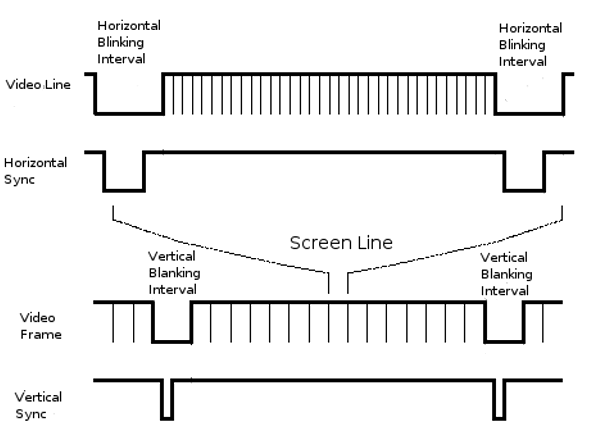
\includegraphics[width=0.7\textwidth]{Grundlagen/vga_timing.png}
	\caption{VGA-Timing, Quelle: \cite{Valcarce2011}}
	\label{fig:vga_timing}
\end{figure}

\subsection{DVI}
Hinter DVI steht der Begriff Digital Visual Interface und stellt ein digitale Schnittstelle zur Grafikanzeige dar. Der DVI Standard wurde 1999 von der DDWG\footnote{Digital Display Working Group} verabschiedet, da der Wunsch nach Leistungsstärkeren Schnittstellen vorhanden war. QXGA-Auflösungen\footnote{QXGA: 2048x1536} sind auf analogem Wege nicht mehr befriedigend erzielbar. Die DVI Schnittstelle beinhaltet neben den Digitalen Signalen zusätzlich analoge VGA Signale, was den Betrieb älterer Monitore und Displays zulässt. Zur digitalen Datenübertragung wird der TMDS\footnote{Transition Minimized Differential Signaling - Differentielle Datenübertragung} Standard verwendet, welcher die 24 Bit Farbinformationen\footnote{24 Bit: je 8 Bit für Rot, Grün und Blau} mittels eines Serializers in serielle Daten umwandelt. Je nach benötigter Bandbreite können drei oder sechs Aderpaare für Pixeldaten verwendet werden. Dies wird Single-Link bzw. Double-Link genannt und es lassen sich dabei max. 3.72 GBit/s\footnote{max. UXGA: 1600x1200@60Hz} bzw. 7.44 GBit/s\footnote{max. WUXGA: 1920x1200@60Hz} übertragen. Um die Paare zuordnen zu können, wird ein weiteres Paar zur Synchronisation verwendet. Um die Übertragung noch effizienter zu gestalten, gibt es die Möglichkeit bei High- sowie Low-Pegel des Taktsignals Daten zu übertragen\footnote{\textit{Double Data Rate}} (\cite{Leunig2002}).

\subsection{HDMI}
Gegeneber der DVI-Schnittstelle bietet die HDMI Schnittstelle dieselben Eigenschaften bezüglich der Videoübertragung verwendet zur ebenfalls TMDS. Hinzu kommt allerdings, dass sowohl Audio als auch Verschlüsselung unterstützt werden. Der Formfaktor der Stecker sind für den Hausgebrauch verkleinert worden. HDMI wurde als normierte Universallösung entwickelt und hat sich als solche etabliert (\cite{Extron2014}). Nahezu jedes neu entwickelte Gerät mit Anzeigemöglichkeit, bietet eine HDMI-Schnittstelle - ebenso embedded Linux Boards wie z.B. bekannte Linux Boards wie Raspberry Pi oder Beagle Bone Black.

\subsection{RGB}
Der RGB-Bus, verwendet für kleine TFT-Panels bis ca. 7", funktioniert prinzipiell analog zur VGA-Schnittstelle, mit dem Unterschied, dass die Datenleitungen komplett digital sind. 
So werden die Signale für Rot, Grün und Blau nicht mehr analog im Bereich von 0V bis +0.7V dargestellt, sondern durch einen üblicherweise acht Bit breiten Bus pro Farbkanal. Die Auflösung pro Farbkanal ist mit 255 Intensitätsstufen gerechnet ausreichend um ein gesamtes Farbspektrum von 16777216 \footnote{16777216 Farben = 2\textasciicircum24} Farben zu erhalten. 
\begin{figure}[htp]
	\centering
	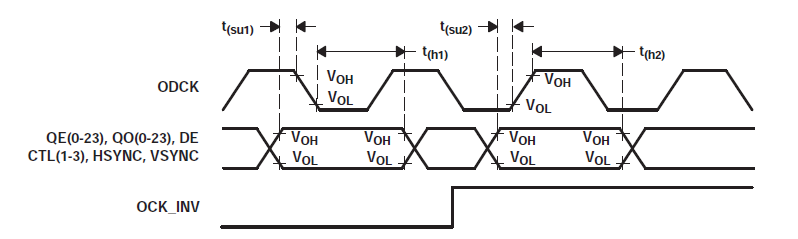
\includegraphics[width=0.8\textwidth]{Grundlagen/rgb_timing.png}
	\caption{RGB-Timing, Quelle: \cite{TI2011}}
	\label{fig:rgb_timing}
\end{figure}
Dieser Farbmodus wird auch RGB888 genannt, da acht Bit für jede Farbe zur Kodierung, insgesamt also 24 Bit, zur Verfügung stehen. Neben dem 24 Bit Modus ist RGB565 noch weit verbreitet, der je fünf Bit für Rot und Blau und sechs Bit für Grün verwendet. Hier ergibt sich ein Farbspektrum von 65536\footnote{65536 = 2\textasciicircum16} Farben. Da digital übertragen wird, ist eine Taktleitung notwendig um die Synchronizität zu ermöglichen. 
Aufgrund der Verbreitung und Mächtigkeit der Schnittstelle besitzen einige Prozessor, wie z.B. der Linuxfähige OMAP3530 von Texas Instruments, eine RGB-Schnittstelle. 
\refa{fig:rgb_timing} zeigt exemplarisch ein Timing-Diagramm der RGB-Schnittstelle des Bausteins TFP-401A von Texas Instruments.
\subsection{LVDS}
Um lange Strecken und große Bildformate übertragen zu können ist der parallele Datentransfer ungeeignet, da bei schnellem Takt z.B. das Übersprechen zu groß wird und das Signal schneller gestört wird. Deshalb ist die Praktik beliebt, große Datenmengen über eine differentielle Verbindung wie z.B. LVDS\footnote{LVDS: Low Voltage Differential Signaling} zu übertragen. Die physikalische Funktionsweise der LVDS Leitung liegt darin, dass zweimal dasselbe Signal übertragen wird - mit positiver Spannung und mit negativer Spannung. Wirkt nun von außen eine Störung auf die LVDS Leitung, werden beide Leitungen - positive wie auch die negative - gleichermaßen gestört. Durch das Zusammenführen beider Signale am Ende, kompensieren sich diese Störungen im Idealfall zu Null. Wie auch LVDS arbeitet das zuvor genannte TMDS ähnlich, da es sich hierbei auch um eine differentielle Übertragungsart handelt. Der Unterschied liegt in der Verwendung. TMDS wird oft eingesetzt, sobald das Signal das Gerät verlässt - z.B. Desktop-Bildschirm mit Anschlusskabel. Befindet sich das Anzeigegerät allerdings im selben Gehäuse, so wird oft LVDS eingesetzt. Neben Bilddaten ist es natürlich auch möglich andere Nutzdaten wie z.B. Sensordaten zu übertragen. 
Aufgrund der hohen Geschwindigkeit und geringen Fehlerrate werden differentiellen Übertragungen werden gerne für Displays angewendet.
\subsection{8080-Interface}
Das 8080-Interface ist eine antike Schnittstelle ursprünglich von Intel 8080 Prozessor. Sie wird bis heute verwendet, um Speicher, kleine TFT-Displays oder andere Bausteine mit einem Mikrocontroller zu betreiben. Eckdaten des 8080-Interface sind sowohl der Datenbus selbst als auch der Adressbus mit z.B. acht, 16 oder 32 Bit, je eine eine Leitung für Read-Enable, Write-Enable und Chip-Select. Durch die Verwendung der Chip-Select Leitungen ist es möglich mehrere Teilnehmer am selben Bus zu betreiben. Alle Teilnehmer, deren Chip-Leitung nicht aktiv ist, verhalten sich für andere Busteilnehmer unsichtbar. Erst mit Zuweisung der Chip-Selects werden diese sichtbar und übernehmen den Bus. Ein Hostsystem steuert als sog. Master die am Bus hängenden Slaves. Moechte das Hostsystem von einem Slave Daten lesen, wird ein Lesezyklus initiiert, der die Chip-Select Leitung aktiviert, die gewünschte Adresse an den Bus anlegt, die Read-Enable Leitung aktiviert und nach einer festgelegten Zeit diese wieder deaktiviert. Der Slave legt die gewünschten Daten auf den Datenbus und der Host kann diese Daten korrekt lesen. Analog dazu funktioniert der Schreibzyklus ähnlich. 
\refa{fig:8080_timing} zeigt das Timing Diagramm eines Schreib- und Lesezyklus des Displaycontrollers SSD1289. Das Signal D/C wird verwendet um zu unterscheiden, ob ein Daten oder ein Kommando auf dem Bus anliegen. Dazu kann beispielsweise eine Adressleitung des 8080-Bus verwendet werden. CS stellt das Chip-Select dar. WR und RD beziehen sich auf Write- bzw. Read-Enable. D0-D17 sind 18 Datenbits des Bus (\cite{SSD2007}). 
\begin{figure}[htp]
	\centering
	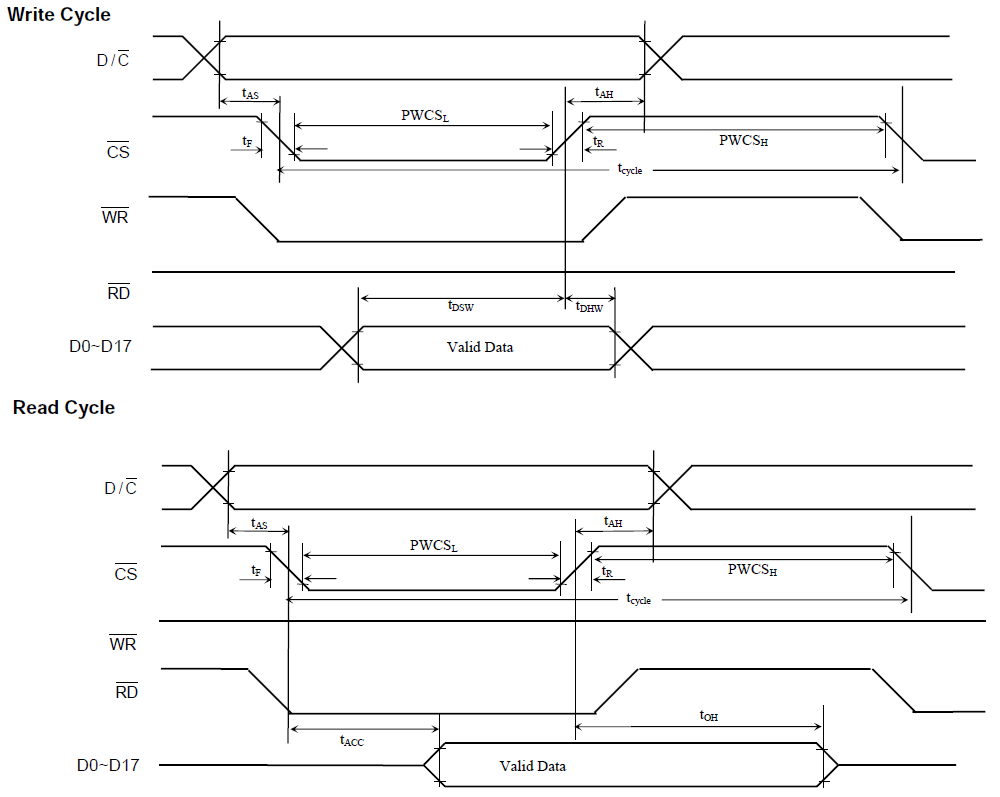
\includegraphics[width=1.0\textwidth]{Grundlagen/8080_timing.png}
	\caption{8080-Timing des SSD1289, Quelle: \cite{SSD2007}}
	\label{fig:8080_timing}
\end{figure}


Viele Mikrocontroller besitzen bereits ein 8080-Interface dediziert in Hardware - allerdings nicht alle. Als Ersatz kann das Protokoll mit GPIO\footnote{GPIO: General Purpose In/Output} in Software implementiert werden. Dies ist allerdings wesentlich langsamer als eine Lösung, die bereits in Hardware läuft, da GPIO-Pins nicht dafür geschaffen sind, sich mit schneller Frequenz schalten zu lassen.
\clearpage

\subsection{Bewertung der Video-Schnittstellen}
Nachdem nun die wichtigsten Schnittstellen dargestellt wurden, werden diese im Folgenden mit dem Fokus auf die Masterareit hinsichtlich der Relevanz bewertet.
Da die VGA-Schnittstelle antik und obsolet ist, spielt sie heutzutage nur noch eine geringe Rolle. Insbesondere im Bereich der embedded Systeme wird sie kaum verwendet. Für die Masterarbeit ist die VGA-Schnittstelle uninteressant, da diese von keiner, in der Masterarbeit behandelten, Hardware verwendet wird. Jedoch wurde diese eingangs behandelt, da diese den Übergang zum digitalen RGB-Bus schafft.\\
Die DVI- und HDMI-Schnittstellen, welche für den Bereich der Videoanzeige praktisch identisch sind, nehmen jedoch einen hohen Stellenwert in der Masterarbeit ein. Im zweiten Teil der Arbeit wird eine Hardware entwickelt, welche als Eingangssignale die TMDS der DVI-/HDMI-Schnittstelle nutzt. 
Ebenso spielen die RGB-Schnittstelle und LVDS eine große Rolle\todo{große Rolle: umschreiben}, da an diesen Schnittstellen der entwickelten Hardware TFT-Panels angeschlossen werden. \\
Neben den reinen Video-Schnittstellen weist das beschriebene 8080-Interface, das ursprünglich nicht zur Bildübertragung gedacht war, ein hohes Potential auf und besitzt für den ersten Teil der Masterarbeit hohen Stellenwert. Gerade im embedded Bereich besitzt diese Schnittstelle nach wie vor einen hohen Stellenwert, da vor allem kleine Displays damit hinreichend schnell und effizient betrieben werden können. \reft{tab:interface_vergleich} zeigt nochmals eine kurze Übersicht der Relevanz der einzelnen Schnittstellen fuer die Masterarbeit.

\begin{table}
\begin{tabular}{|c|c|c|}\hline
   Schnittstelle & Relevanz für Masterarbeit & Verwendung in der Masterarbeit\\ \hline
   VGA & keine  & - \\               \hline
   DVI & mittel & Teil B \\          \hline
   HDMI & hoch	& Teil B \\          \hline
   RGB & hoch & Teil B \\            \hline
   LVDS & hoch & Teil B \\           \hline
   8080-Interface & hoch & Teil A \\ \hline
\end{tabular}
\caption{Relevanz der Display-Schnittstellen für die Masterarbeit}
\label{tab:interface_vergleich}
\end{table}

\section{Betrachtete Embedded Linux Boards}
In diesem Abschnitt werden die verwendeten Linux-Boards dargestellt, verglichen und hinsichtlich der Verwendbarkeit in der Masterarbeit bewertet. Da sich die Masterarbeit in zwei Teile gliedert, wird für beide Anwendungsfaelle ein typisches Linux-Board hergezogen, welches den Anforderungen gerecht werden muss, eine billige und effiziente Anzeige zu gestatten.
\subsection{Raspberry Pi}
Am wohl bekanntesten und mit einer riesigen Community hinter dem Projekt ist der Raspberry Pi von der Raspberry Pi Foundation \footnote{\url{http://www.raspberrypi.org}}. Um die wichtigsten Eckdaten des Einplatinenrechners im Checkkartenformat zu nennen, besitzt er in der Ausfuehrung Model B einen ARM11-Core (Broadcom BCM2835), 512 Megabyte SDRAM, eine Broadcom VideoCore IV GPU sowie diverse Schnittstellen wie HDMI, USB 2.0, UART\footnote{UART: Universal Asynchronous Receiver Transmitter - RS2332}, SPI\footnote{SPI: Serial Peripheral Interface - 4 Draht Bus}, I2C\footnote{I2C: Inter Integrated Circuit - 2 Draht Bus} sowie GPIO-Pins\footnote{GPIO: General Purpose Input Output}.\\
Der erschwingliche Preis macht den Raspberry Pi attraktiv und zieht die Community an, da man für rund 40 Euro einen kompletten Rechner bekommt. \\
\begin{tabular}{|c|c|}\hline
   Lehrstuhl & Professor \\ \hline
   BWL & Maier \\ \hline
   MB & M"uller \\ \hline
   Jura & Schmidt \\ \hline
 \end{tabular}


\subsection{Gnublin Extended}


\subsection{Bewertung der Linux-Boards}

\chapter{Teil A}
\label{cha:TeilA}
Im Folgenden Kapitel wird Teil A dieser Arbeit behandelt. Es wird die Ansteuerung von TFT Displays über den 8080-Bus auf Basis des Gnublin Linuxboards realisiert. Hierzu wurden verschieden große LCD Displays mit unterschiedlichen Controllern unter Verwendung des 8080-Interface und untersucht. 

\section{Untersuchte Displays mit 8080-Interface}
Dieser Abschnitt behandelt die untersuchten Displays. Es wurden drei Displays aus China untersucht. Der Fokus bei der Bestellung lag vor allem darauf, dass die Pinbelegung der jeweiligen Displays übereinstimmen. So ist die Entwicklung von nur einer Adapterplatine zwischen Gnublin und Display nötig. Alle verwendeten Displays werden im 16 Bit Farbmodus betrieben. Die hieraus resultierende Farbtiefe beträgt 65.535 Farben.\newline % \footnote{2^16 = 65.536}
Alle verwendeten Displays arbeiten dahingehend gleich, dass sie Kommandos und Daten auf dem Datenbus anliegen, diese jedoch durch eine gesonderte Leitung unterschieden werden. Soll dem Display also etwas mitgeteilt werden, so muss zuerst ein entsprechendes Kommando und im Anschluss die Nutzdaten gesendet werden. Um Pixeldaten an das Display zu senden, hat sich die Vorgehensweise etabliert, eine Rechteckige Region im RAM des Displays zu reservieren, das durch die 4 Eckpunkte des Rechtecks definiert sind. Werden im Anschluss Pixeldaten gesendet, inkrementiert der Controller die Adresse automatisch und springt bei einem Zeilenumbruch automatisch an die richtige Stelle im RAM. Der maximale Speicher im Controller beschränkt die maximale Auflösung der ansteuerbaren TFT-Panel. Trotz der Tatsache, dass sich die Displays auf elektrischer Seite nicht unterscheiden, so müssen diese allerdings alle speziell softwareseitig behandelt werden. \todo{bild von Ramfenster hinzufuegen}

\subsection{4.3"'/5"' mit SSD1963}
Die Wahl des Controllers SSD1963 von Solomon Systech liegt nahe, da dieser bereits mit einem 4.3"'  Panel in einer vorausgehende Arbeit verwendet wird. Dort ist das Display mittels GPIO-Pins am Raspberry Pi angeschlossen. Die Software bezüglich der reinen Displayansteuerung ist somit bereits vorhanden (siehe \cite{Schlegel2013a}). Aufgrund eines Problems, das in Abschnitt \ref{cha:TeilAKnownBugs_SSD1963} näher beschrieben ist, wird für diese Arbeit zusätzlich ein anderes Display mit 5"' Panel aber selbem Controller untersucht. 
\refa{fig:8080_pinout} zeigt das Pinout der verwendeten Displays (Quelle: \cite{Coldtears2014}).
\begin{figure}[h]
	\centering
\fbox{	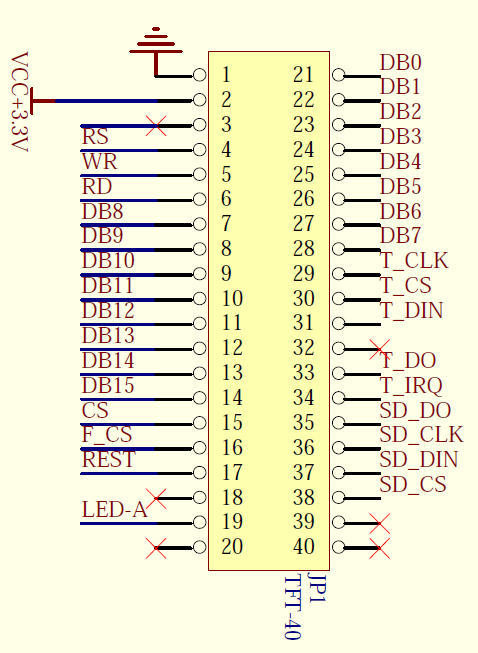
\includegraphics[width=0.5\textwidth]{TeilA/display_pinout.png}}
	\caption{8080-Display Pinout}
	\label{fig:8080_pinout}
\end{figure}
Die Displays besitzen bei 4.3"' eine Auflösung von 480x272 beziehungsweise bei 5"' 800x480 Pixeln. Neben den für die Initialisierung nötigen Kommandos besitzt der Controller folgende wichtigen Kommandos. Diese sind in \reft{tab:Kommandos_SSD1963} beschrieben (Quelle:  \cite{SSD2008}). Die zur Initialisierung notwendigen Kommandos werden hier nicht erläutert, da diese aus dem Datenblatt entnehmbar sind.
\begin{table}[h]
\begin{tabular}{|p{4cm}|p{1cm}|p{8cm}|}\hline
\rowcolor{TableBackgroundColor} 
   \textbf{Kommando} & \textbf{Hex-Code} & \textbf{Kommentar}\\ \hline
   Set Column Address & 0x2A & Eckpunkte des RAM-Fensters in X-Richtung \\ \hline
   Set Page Address & 0x2B & Eckpunkte des RAM-Fensters in Y-Richtung \\ \hline
   Write Memory Start & 0x2C & Alle Folgenden Pixeldaten werden im RAM-Fenster platziert \\ \hline
\end{tabular}
\caption{Relevante Kommandos des SSD1963}
\label{tab:Kommandos_SSD1963}
\end{table}


\subsection{3.2"' mit SSD1289}
Das 3.2"' Display von Sainsmart wird mit einen SSD1289 von Solomon Systech betrieben. Dieses Display hat eine Aufloesung ovn 320x240 Farbpunkten. Das Pinout ist dasselbe, das in \refa{fig:8080_pinout}MPMCStatic zu sehen ist. Analog zu \reft{tab:Kommandos_SSD1963} besitzt der SSD1289 seine eigenen wichtigen Kommandos. Diese sind in  \reft{tab:Kommandos_SSD1289} erläutert (siehe \cite{SSD2007}). Die zur Initialisierung notwendigen Kommandos werden hier nicht erläutert, da diese aus dem Datenblatt entnehmbar sind.
\begin{table}[h]
\begin{tabular}{|p{4cm}|p{1cm}|p{8cm}|}\hline
\rowcolor{TableBackgroundColor}
   \textbf{Kommando} & \textbf{Hex-Code} & \textbf{Kommentar}\\ \hline
   Horizontal RAM address position & 0x44 & Eckpunkte des RAM-Fensters in X-Richtung \\ \hline
   Vertical RAM address start position & 0x45 & Startpunkt des RAM-Fensters in Y-Richtung \\ \hline
   Horizontal RAM address stop position & 0x46 & Endpunkt des  RAM-Fensters in Y-Richtung \\ \hline
   Set GDDRAM X address counter & 0x4E & Zeiger im  RAM-Fenster in X-Richtung \\ \hline
   Set GDDRAM Y address counter & 0x4F & Zeiger im RAM-Fenster in Y-Richtung \\ \hline
   RAM Write  Register & 0x22 & Alle Folgenden Pixeldaten werden im RAM-Fenster platziert \\ \hline
\end{tabular}
\caption{Relevante Kommandos des SSD1289}
\label{tab:Kommandos_SSD1289}
\end{table}


\subsection{5"' mit CPLD}
Als drittes Display mit 8080-Interface kommt eine 5"' Display mit einer Auflösung von 800x480 Bildpunkten zum Einsatz, dass keinen univerell einsetzbaren Controller für variable Displaypanels im klassischen Sinn besitzt, sondern ein CPLD \footnote{CPLD: Complex Programmable Logic Device} als Controller mit zugeschnittenen Timings für das verwendete TFT-Panel. Der Vorteil eines solchen Displays ist, dass keine Initialisierungsroutine benötigt wird, um die Timings für das Panel einzustellen. Ein Reset setzt das Display betriebsbereit. Nachteilig stellt sich der Umstand ein, dass nur TFT-Panels exakter Größe und mit exakten Timings verwendet werden können. Für diese Arbeit ist allerdings die Verwendung von anderen Panels belanglos. Auch hier ist das Pinout des Displays analog zu dem Gezeigten in \refa{fig:8080_pinout}.\newline
Wichtige Kommandos zum Betrieb des Displays sind in \reft{tab:Kommandos_MD050SD} einsehbar (siehe \cite{ITEAD2013}). Dieses Display trägt die Bezeichnung MD050SD.

\begin{table}[h]
\begin{tabular}{|p{4cm}|p{1cm}|p{8cm}|}\hline
\rowcolor{TableBackgroundColor}
   \textbf{Kommando} & \textbf{Hex-Code} & \textbf{Kommentar}\\ \hline
   Beginning Row Address & 0x02 & Startpunkt des RAM-Fensters in X-Richtung \\ \hline
   Ending Row Address& 0x06 & Endpunkt des RAM-Fensters in X-Richtung \\ \hline
   Beginning Column Address & 0x03 & Startpunkt des RAM-Fensters in Y-Richtung \\ \hline
   Ending Column Address& 0x07 & Endpunkt des RAM-Fensters in Y-Richtung \\ \hline
   Writing Page Register & 0x05 & Alle Folgenden Pixeldaten werden im RAM-Fenster platziert \\ \hline
\end{tabular}
\caption{Relevante Kommandos des MD050SD}
\label{tab:Kommandos_MD050SD}
\end{table}

% \section{8080-Interface mittels GPIO-Pins}
\label{sec:TeilA_8080GPIO}

\subsection{Konzept}
\subsection{Hardwareverbindung zwischen GPIO-Pins und Display}
\subsection{User-Space-Treiber}
\subsubsection{Low-Level-Treiber}
\paragraph{GPIO-Pin Frequenz erhoehen}
\paragraph{GPIO-Treiber}
\paragraph{Displaytreiber fuer SSD1963}
\subsection{Ansteuerung des Displays}



\section{8080-Interface mittels SRAM-Interface}
\label{sec:TeilA_8080SRAM}
Wie bereits in \refc{cha:gnublin_extended} erwaehnt, besitzt der Prozessor des Gnublin bereits ein externes 8080-Interface, auf welches zugegriffen wird. Im Folgenden wird auf das Konzept, die Idee und die Realisierung auf Hardware- und Softwareseite eingegangen.
\newpage
\subsection{Konzept}
\label{cha:teila_konzept}
Im Gnublin stellt ein NXP LPC313x die zentrale Recheneinheit dar. Dieser besitzt ein sogenanntes EBI \footnote{EBI: External Bus Interface}, worüber externe Bausteine wie Speicher, Ethernetcontroller oder ähnliche Bausteine angesprochen werden können.

\begin{figure}[htp]
%\begin{minipage}[t]{0.8\textwidth}
%\begin{figure}[h]
	\centering
\fbox{	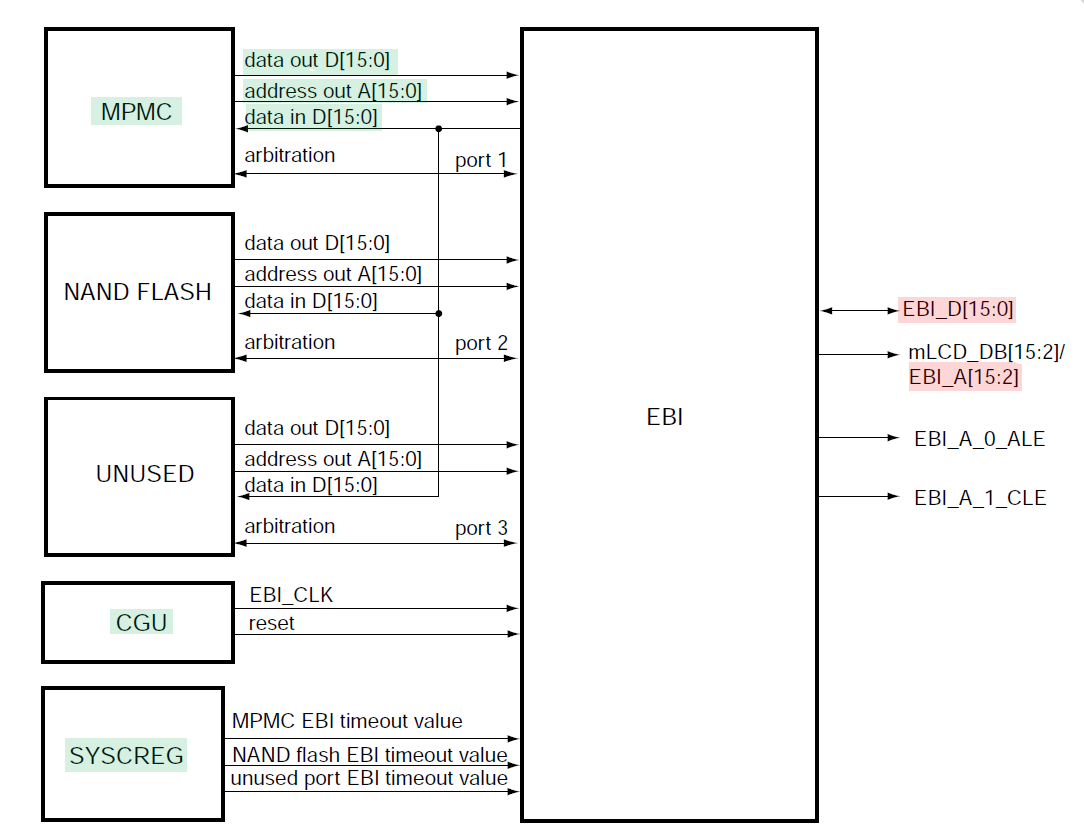
\includegraphics[width=1.0\textwidth]{TeilA/lpc_ebi.png}}
	\caption{NXP LPC313x EBI, Quelle: \cite{NXP2010}}
	\label{fig:lpc_ebi}
\end{figure}
%\end{minipage}

In \refa{fig:lpc_ebi} ist ein Blockschaltbild des EBI zu sehen, bei welchem neben CGU \footnote{CGU: Clock Generation Unit, Takterzeugung} und SYSCREG\footnote{SYSCREG: System Control Register, Steuerregister}, MPMC\footnote{MPMC: Multiport Memory Controller} sowie das NAND Flash an den Eingängen des EBI angeschlossen sind. Abgesehen von NAND Flash sind die Eingänge zum EBI für diese Arbeit relevant und grün markiert. An den Ausgängen des EBI sind Adress- und Datenbus zum Anschluss an externe Bausteine herausgeführt. Damit verschiedenartigen Bausteine an denselben Adress- und Datenpins angeschlossen werden kann, ist eine Priorisierung notwendig. Die Höchste Priorität besitzt der MPMC, gefolgt vom NAND Flash. 
Die Grundidee ist, das Display über den MPMC anzuschließen, da er so konfiguriert werden kann, dass er sich 8080-konform verhält. Die für diese Arbeit interessanten Leitungen am Ausgang des EBI sind mit rot markiert. Hier wird der Datenbus selbst, sowie die oberen 13 Bit des Adressbus gezeigt.


\subsection{MPMC - Multiport Memory Controller des NXP LPC313x}
\label{cha:mpmc}

Der MPMC stellt die Möglichkeit zur Verfügung Bausteine wie dynamisches und statisches RAM anzubinden. Die Refresh-Zyklen werden bei Verwendung von dynamischen RAMs automatisch vollzogen. Das SDRAM-Interface bietet von Haus aus die Möglichkeit Displays mit 8080-Interface zu betreiben. Dies schließt allerdings die Verwendung von dynamischen RAMs aus. Soll ein Betriebssystem wie Linux auf dem System betrieben werden, ist allerdings die Verwendung von dynamischem RAM unerlässlich. Im Folgenden wird die Schnittstelle für das statische RAM SRAM-Interface benannt. Es besteht die Möglichkeit das Interface des statischen RAM zu verwenden, um ein Display zu betreiben, da es sich so konfigurieren lässt, dass es sich wie ein 8080-Interface verhält. Damit sich die verschiedenen Slaves an Adress- und Datenbus nicht überschneiden, regelt das EBI den Zugriff auf die Busse über Chip-Select Leitungen. Am Gnublin ist eine dieser Chip-Select-Leitungen für das SRAM-Interface nach außen gelegt. Die restlichen Anschlüsse wie Write-Enable, Read-Enable, Reset sind ebenfalls herausgeführt \cite{NXP2010}. Ein Blockschaltbild des MPMC ist in \refa{fig:lpc_mpmc} zu sehen.


\begin{figure}[tbph]
%\begin{figure}[h!]
	\centering
\fbox{	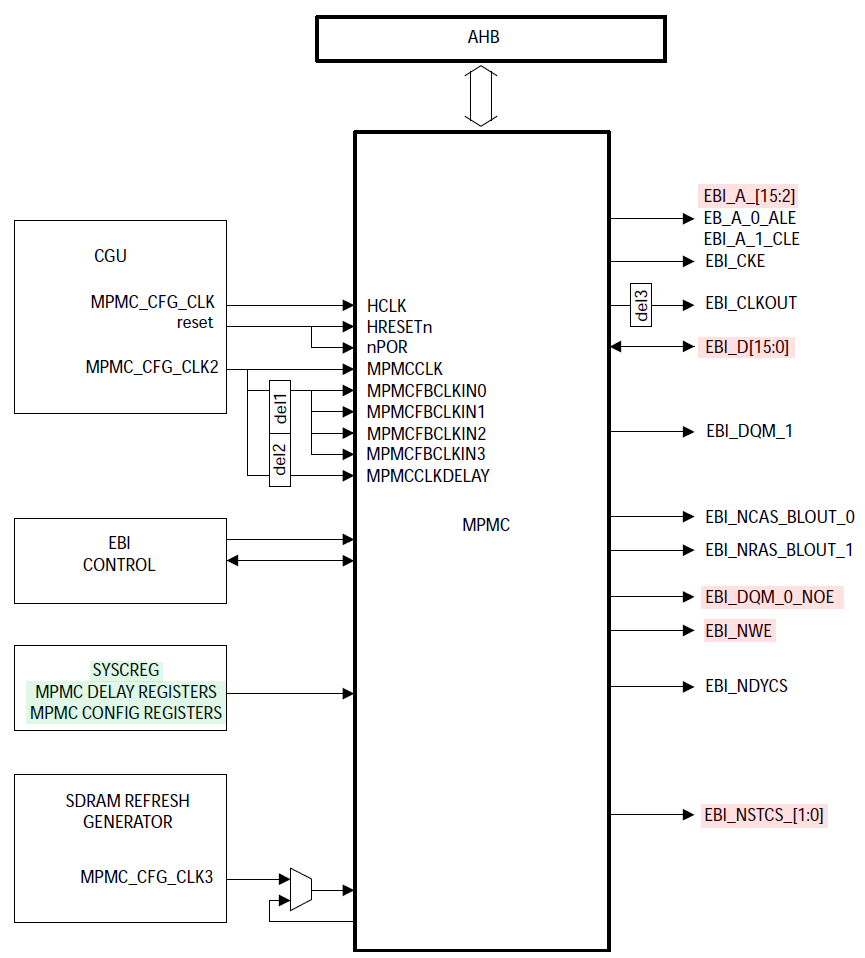
\includegraphics[width=1.0\textwidth]{TeilA/lpc_mpmc.png}}
	\caption{NXP LPC313x MPMC, \cite{NXP2010} }
	\label{fig:lpc_mpmc}
\end{figure}
\newpage
Die Register des MPMC werden so konfiguriert, dass die Schnittstelle kompatibel zum Display und dessen Timings wird. Entsprechend dem verwendeten Chip-Select-Signal werden die Register \begin{itemize}
\item MPMCStaticConfig0\item  MPMCStaticWaitWen0\item  MPMCStaticWaitOen0\item  MPMCStaticRd0\item  MPMCStaticPage0\item  MPMCStaticWr0 \item MPMCStaticWaitTurn0 \end{itemize} konfiguriert. Die Basisadresse des MPMC ist 0x1700 8000. Wie die Register zu beschreiben sind, geht aus \cite{NXP2010} auf Seite 56 hervor und ist in \reft{tab:mpmc_config} gezeigt. Die Timings wurden so gewählt, dass die Timinganforderungen der Displaycontroller eingehalten werden.

\begin{table}[h]
\begin{tabular}{|p{4cm}|p{1cm}|p{1cm}|p{6.6cm}|}\hline
\rowcolor{TableBackgroundColor} 
	\textbf{Register} 	& \textbf{Offset} 	& \textbf{Wert} & \textbf{Beschreibung} 							\\ \hline
	MPMCStaticConfig0 	& 0x200 		& 0x81 			& \begin{itemize}
	\item 16 Bit Modus \item Aktiviert die Nutzung von EBI\_nWE \item  CS low aktiv\item  keine ExtendedWait-Zyklen\item  Schreibpuffer deaktiviert\item  Geschütztes Schreiben deaktiviert \item Page Mode deaktiviert 	\end{itemize} 	\\ \hline
	MPMCStaticWaitWen0 	& 0x204 		& 13 			& 13 + 1 = 14 Wartezyklen ab Chip-Select bis Write-Enable 	\\ \hline
	MPMCStaticWaitOen0 	& 0x208 		& 0 			& 0 + 1 = 1 Wartezyklus ab Chip-Select bis Output-Enable  												\\ \hline
	MPMCStaticRd0 		& 0x20C 		& 0 			& 0 + 1 = 1 Wartezyklus ab Chip-Select bis Read-Enable					\\ \hline
	MPMCStaticPage0 	& 0x210 		& 0 			& 0 + 1 = 1 Wartezyklus für sequential Page Mode Access												\\ \hline
	MPMCStaticWr0 		& 0x214 		& 15 			& 15 + 2  = 17 Wartezyklen bis Write-Access	\\ \hline
	MPMCStaticWaitTurn0 & 0x218 		& 0 			& 0 + 1 = 1 Turnaround Cycles 								\\ \hline
\end{tabular}
\caption{MPMC Register, \cite{NXP2010}}
\label{tab:mpmc_config}
\end{table}
\newpage

Neben den MPMC-Registern muss das Register SYSCREG\_AHB\_MPMC\_MISC konfiguriert werden. Wird Bit 7 des Registers  auf der Adresse 0x1300 2864 mit dem Wert 0 eingestellt, so verändert sich das Adressierungsverhalten dahingehend, dass sich die Adressleitungen des EBI EBI\_A[15:0] auf den für den Prozessor sichtbaren AHB\footnote{AHB: Advanced Microcontroller Bus Architecture} Adressbus AHB\_A[16:1] verschiebt (siehe \cite{NXP2010}, S.~485f). Der Prozessor selbst, kann nun also 17 Bit adressieren, jedoch nur im Sprung von zwei Adressen, da das ursprüngliche LSB weggefallen ist.

\newpage
\subsection{Hardwareverbindung zwischen SRAM-Interface und Display}
In diesem Abschnitt wird die Verbindung zwischen dem Prozessor und dem Display behandelt. Eingangs wurde bereits erwähnt, dass beim Kauf der Displays Augenmerk auf Pinkompatibilität gelegt wurde. Das schlägt sich beim Entwurf der Adapterplatine positiv zu Buche, da nun lediglich ein Adapter benötigt wird. \newline
Bereits dargestellt zeigt \refa{fig:8080_pinout} auf Seite \pageref{fig:8080_pinout} das Pinout der verwendeten Displays. Der Anschluss an den Prozessor stellt sich wir in \reft{tab:display_gnublin_verbindung} dar. Anhand der gewonnenen Erkenntnisse aus \refc{cha:teila_konzept} und \refc{cha:mpmc} sowie des Schaltplans des verwendeten Gnublin Extended (siehe \cite{EmbeddedProjects2013}) kann eine Zuordnung getroffen werden. Nicht verbundene Pins sind mit 'nc'\footnote{nc: not connected} vermerkt.

\begin{table}[h]
\begin{tabular}{|p{0.6cm}|p{2.5cm}|p{2.5cm}|p{0.6cm}|p{2.5cm}|p{2.5cm}|}\hline
\rowcolor{TableBackgroundColor} 
\textbf{Nr.}	&	\textbf{Pin Display}	&	\textbf{Pin Gnublin}  & \textbf{Nr.}	&	\textbf{Pin Display}	&	\textbf{Pin Gnublin} 	\\ \hline
1				&	GND						&	GND					  &	21				&	DB0						&	LPC\_DB0				\\ \hline
2				&	+3V3					&	+3V3				  &	22				&	DB1						&	LPC\_DB1				\\ \hline
3				&	nc						&	nc				 	  & 23				&	DB2						&	LPC\_DB2				\\ \hline
4				&	RS						&	LPC\_A15	    	  &	24				&	DB3						&	LPC\_DB3				\\ \hline
5				&	WR						&	LPC\_WE				  &	25				&	DB4						&	LPC\_DB4				\\ \hline
6				&	RD						&	LPC\_DQM0			  &	26				&	DB5						&	LPC\_DB5				\\ \hline
7				&	DB8						&	LPC\_DB8			  &	27				&	DB6						&	LPC\_DB6				\\ \hline
8				&	DB9						&	LPC\_DB9			  &	28				&	DB7						&	LPC\_DB7				\\ \hline
9				&	DB10					&	LPC\_DB10			  &	29				&	nc						&	nc						\\ \hline
10				&	DB11					&	LPC\_DB11			  &	30				&	nc						&	nc						\\ \hline
11				&	DB12					&	LPC\_DB12			  &	31				&	nc						&	nc						\\ \hline
12				&	DB13					&	LPC\_DB13			  &	32				&	nc						&	nc						\\ \hline
13				&	DB14					&	LPC\_DB14			  &	33				&	nc						&	nc						\\ \hline
14				&	DB15					&	LPC\_DB15			  &	34				&	nc						&	nc						\\ \hline
15				&	CS						&	STCS0				  &	35				&	nc						&	nc						\\ \hline
16				&	nc						&	nc					  &	36				&	nc						&	nc						\\ \hline
17				&	RESET					&	GPIO19				  &	37				&	nc						&	nc						\\ \hline
18				&	nc						&	nc					  &	38				&	nc						&	nc						\\ \hline
19				&	LED-A					&	GPIO20				  &	39				&	nc						&	nc						\\ \hline
20				&	nc						&	nc				 	  &	40				&	nc						&	nc						\\ \hline

\end{tabular}
\caption{Displayverbindung mit dem Gnublin, \cite{Coldtears2014}, \cite{EmbeddedProjects2013}}
\label{tab:display_gnublin_verbindung}
\end{table}

Das Daten-Interface des Displays ist mit den Pins DB[0:15] mit dem Datenbus verbunden. Die Signale Read-Enable RD und Write-Enable WR liegen auf den Pins LPC\_DQM0 und LPC\_WE. Als Chip-Select wird das Signal STCS0 verwendet. Diese Pins sind aus dem EBI herausgeführt (siehe \refa{fig:lpc_ebi}) und werden, sofern es das System von der Auslastung am Bus ermöglicht, für das Display zur Verfügung gestellt.

Das RS Signal am Display, welches zwischen Kommando und Daten unterscheidet, liegt auf dem Adresssignal A15. Die folgenden Angaben gehen von einer Registerkonfiguration nach \refc{cha:mpmc} aus. Werden Daten gesendet, so ist der Pin logisch 1, was einem Wert auf dem Adressbus von 0x10000\footnote{0x10000 = 0b0001 0000 0000 0000 0000} entspricht. Bei Kommandos ist der Pin logisch 0 mit einem Adresswert von 0x00000\footnote{0x00000 = 0b0000 0000 0000 0000 0000}. Die unteren 16 Bits des Adressraums lassen sich also willkürlich verändern, da nur das MSB\footnote{MSB: Most Sigificant Bit, das höchstwertige Bit} vom Display verwendet wird. 

Als RS-Pin ist die Adressleitung A15 (logisch verschoben auf A16) gewählt, da so möglicherweise DMA-Transfers\footnote{DMA: Direct Memory Access, Speichertransfer effizient und schnell direkt in Hardware} von bis zu 65.536 Bytes\footnote{65.536 = $2^{16}$} möglich sind. Der DMA-Transfer könnte die Adressleitungen bei Daten von 0x10000 bis 0x1FFFF\footnote{0x1FFFF = 0b0001 1111 1111 1111 1111} bzw. bei Kommandos von 0x0000 bis 0x0FFFF\footnote{0x0FFFF = 0b0000 1111 1111 1111 1111} inkrementieren ohne die Gültigkeit der Wahl zwischen Kommando und Daten des Displays zu beeinträchtigen.

Das Display lässt sich Zusammenfassend also über zwei Pseudoregister für Kommando und Daten auf den Adressoffsets 0x00000 und 0x10000 mit der Basisadresse 0x20000000 ansprechen. Dies ist in \reft{tab:sram_adressen} nochmals übersichtlich dargestellt.

\begin{table}[h]
\begin{tabular}{|p{4.5cm}|p{4cm}|p{4cm}|}\hline
\rowcolor{TableBackgroundColor} 
	\textbf{Register} 	& \textbf{Adresse} 	& \textbf{Typ} 			\\ \hline
	SRAM0\_DISP\_CTRL 	& 0x20000000		& Kommandos				\\ \hline
	SRAM0\_DISP\_DATA 	& 0x20010000 		& Daten 				\\ \hline
\end{tabular}
\caption{Adressen für SRAM-Zugriff, \cite{NXP2010}}
\label{tab:sram_adressen}
\end{table}


Die Untersuchung inwieweit DMA-Transfer praktisch mit der verwendeten Hardware möglich ist, ist allerdings nicht Bestandteil dieser Arbeit. 

\newpage
\subsection{Adapterplatine zwischen Gnublin Extended und Display}
Der Adapter wird als Platine realisiert, die auf den Gnublin Extended aufgesteckt wird. Das Display wiederum wird mit der Adapterplatine steckbar verbunden. Der Schaltplan ist in \refa{fig:adapterplatine_sch} gezeigt und stellt entsprechend \reft{tab:display_gnublin_verbindung} die Verbindungen her.

Der grün markierte Bereich stellt die Verbindung zum Display dar, rot zum Gnublin Extended und im blauen Rechteck sind weitere kleine Bauteile untergebracht. Hier sind Pullup-Wiederstande mit 10~k$\Omega$ an den Leitungen STCS0, Reset und LED-A um definierte Pegel vorzugeben zu sehen sowie einen Blockkondensator mit 100~nF, der für eine bessere Spannungsversorgung des Displays sorgt.

\begin{figure}[tbph]
%\begin{figure}[h!]
	\centering
\fbox{	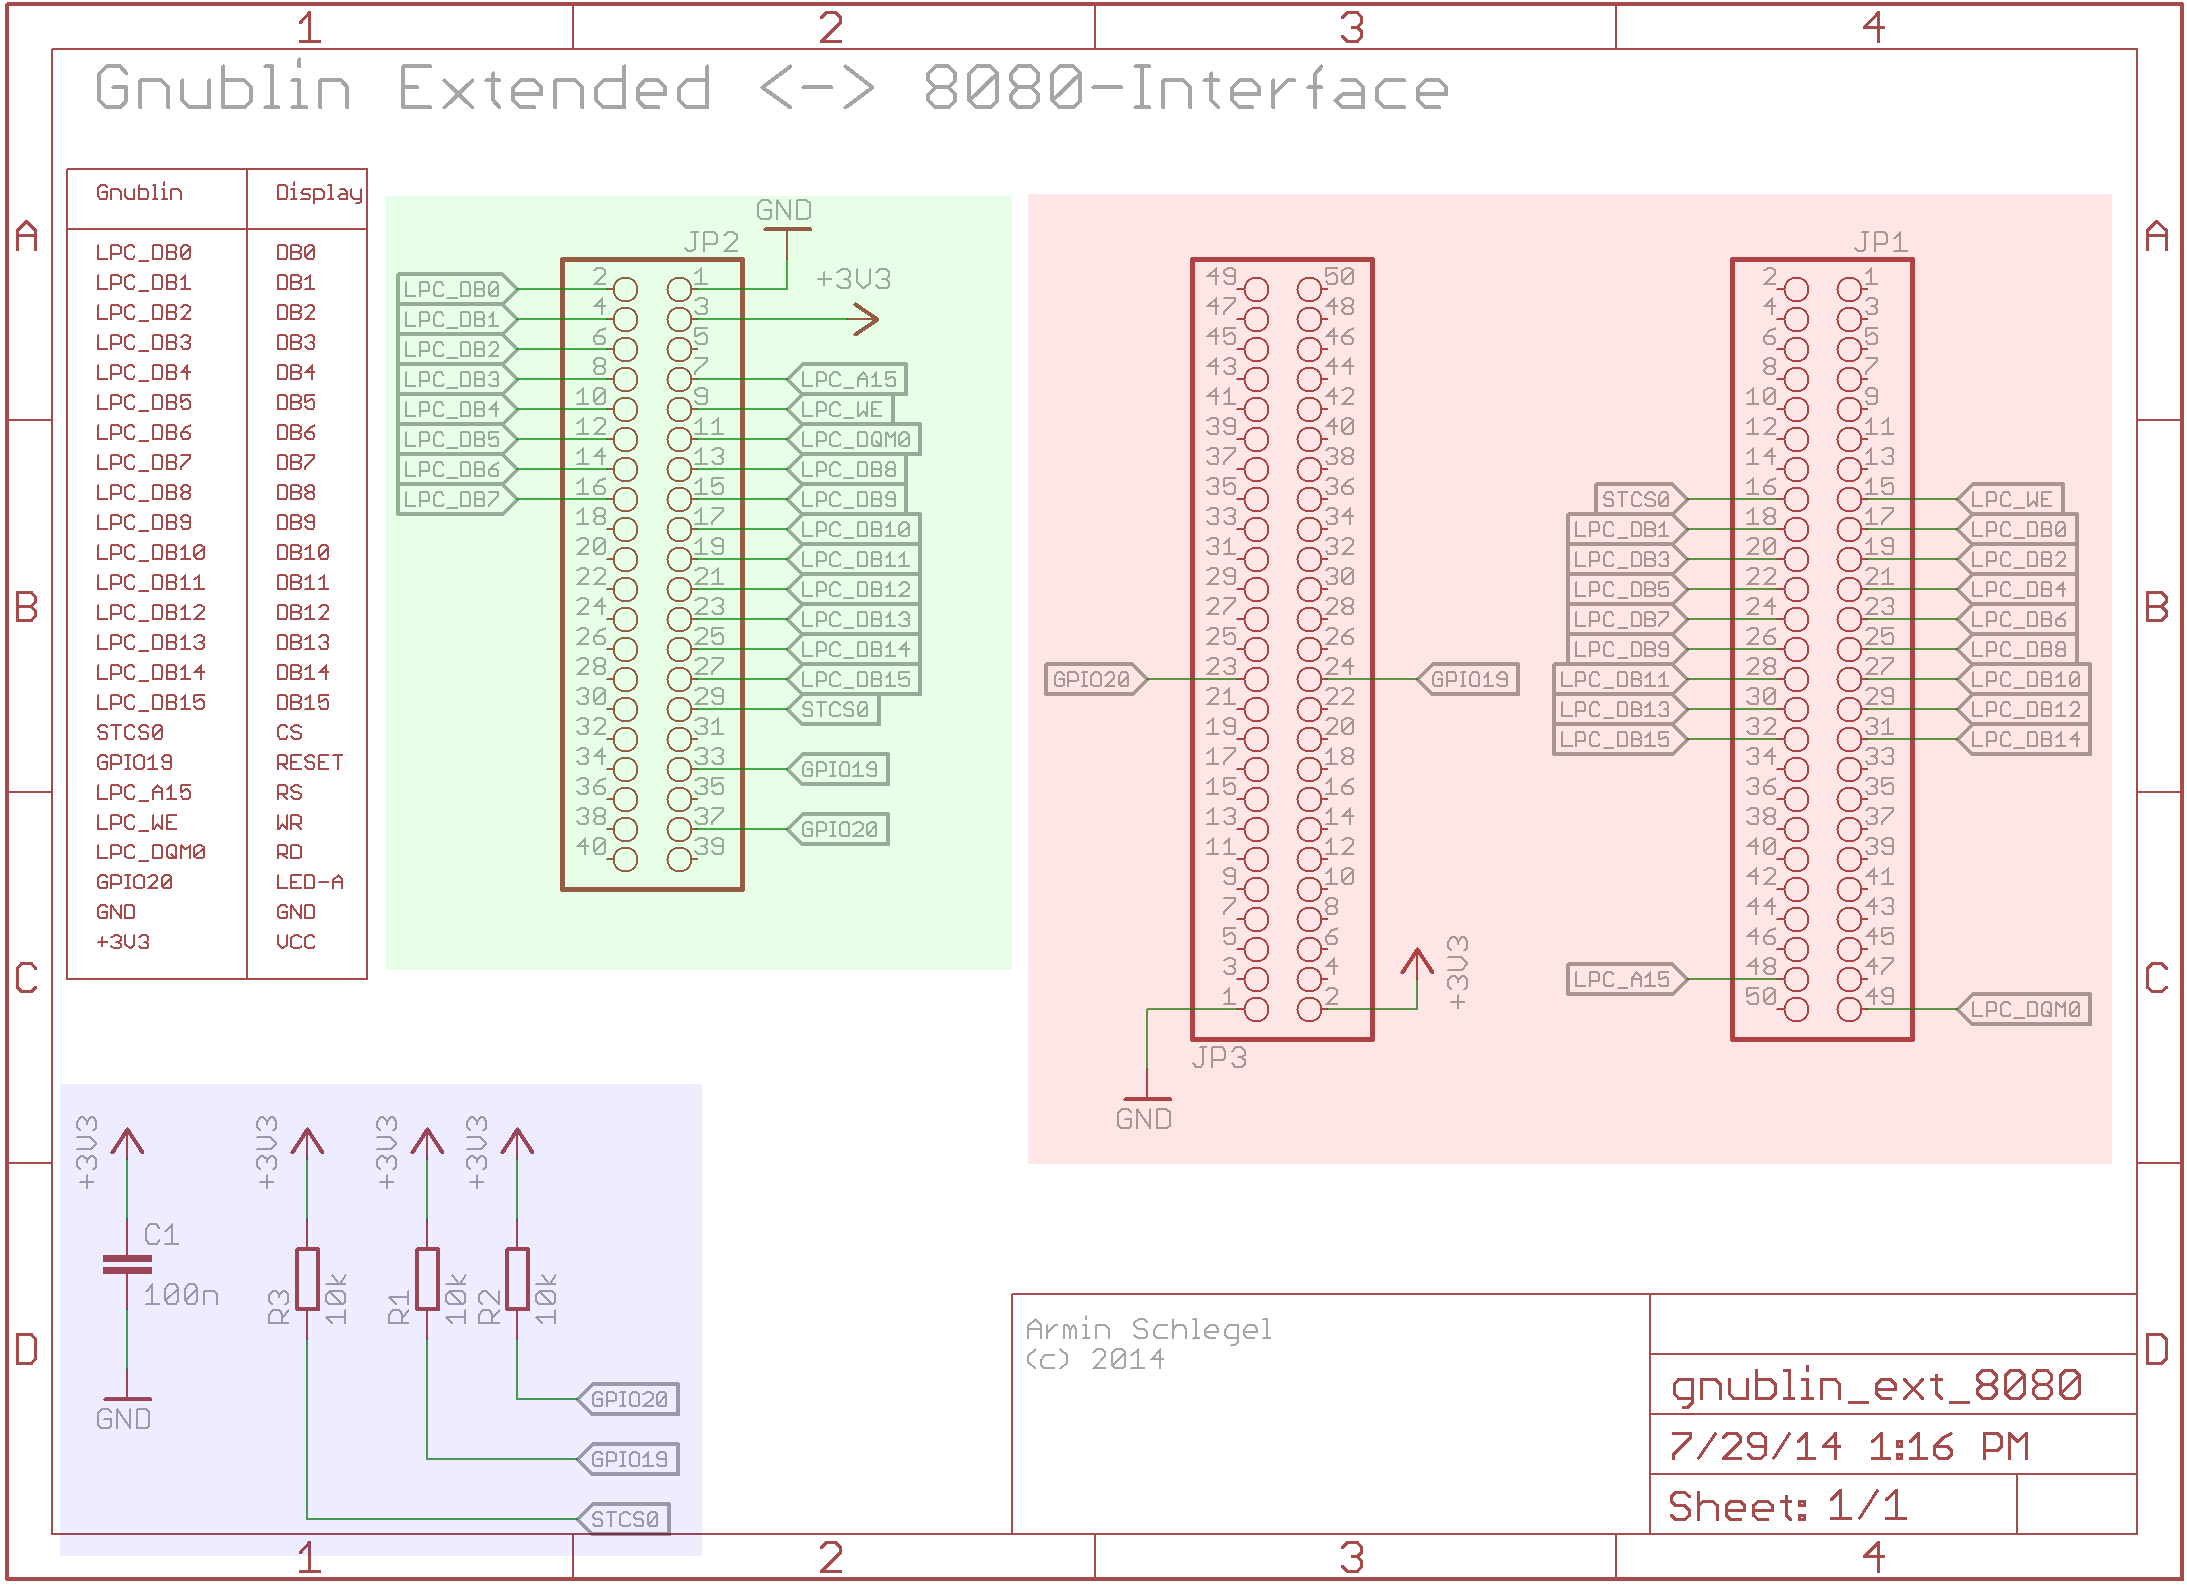
\includegraphics[width=1.0\textwidth]{TeilA/schematic.png}}
	\caption{Schaltplan Adapterplatine}
	\label{fig:adapterplatine_sch}
\end{figure}
\newpage

\refa{fig:adapterplatine} (a) und (b) zeigt je ein gerendertes 3D Bild der Ober- und Unterseite der Adapterplatine. Auf der Oberseite wird das Display auf der linken Seite mit der 40 poligen Stiftleiste angeschossen. Mit der Unterseite wird die Platine auf das Gnublin Extended mit je zwei 50 poligen Buchsenleisten aufgesteckt.

\begin{figure}
        \begin{center}
        \begin{subfigure}[htp]{0.8\textwidth}
                \fbox{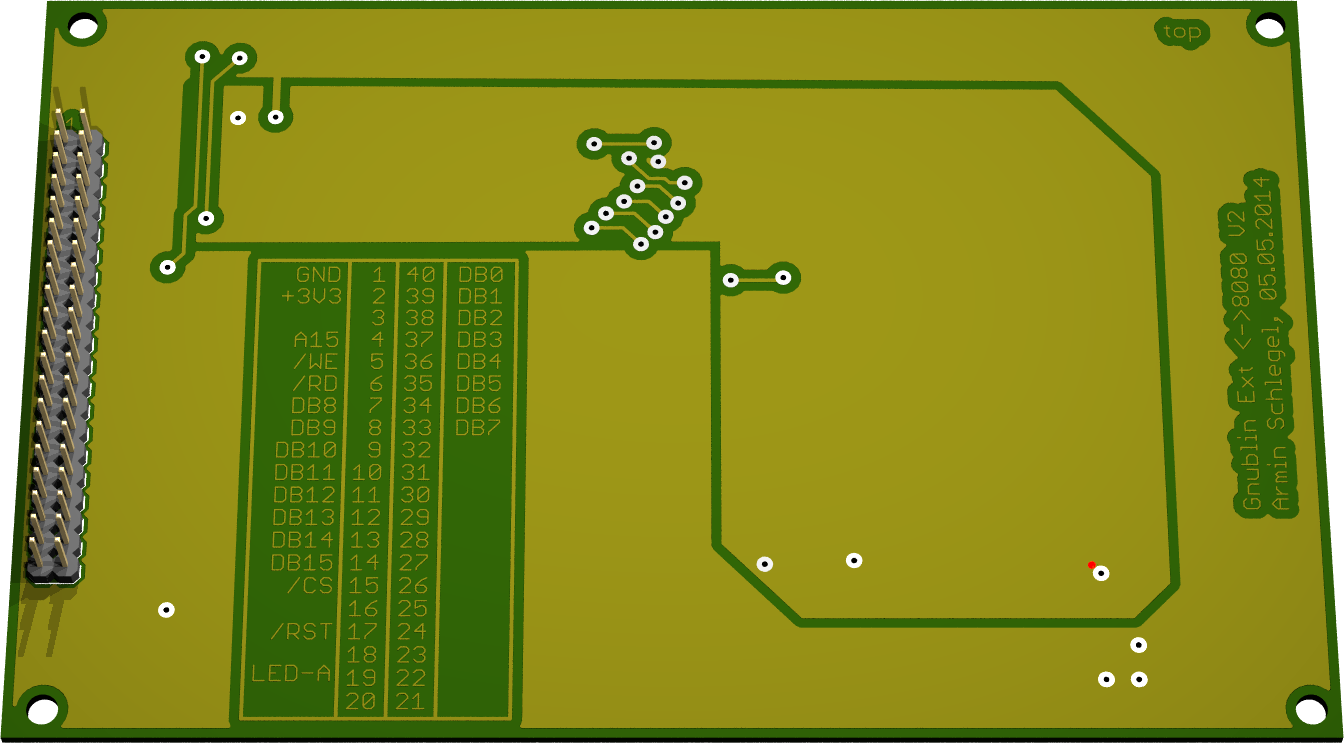
\includegraphics[width=\textwidth]{TeilA/gnublin_ext_ssd1963_top.png}}
                \caption{Adapterplatine Top Layer}
                \label{fig:adapter_top}
        \end{subfigure}

        \begin{subfigure}[htp]{0.8\textwidth}
               \fbox{ 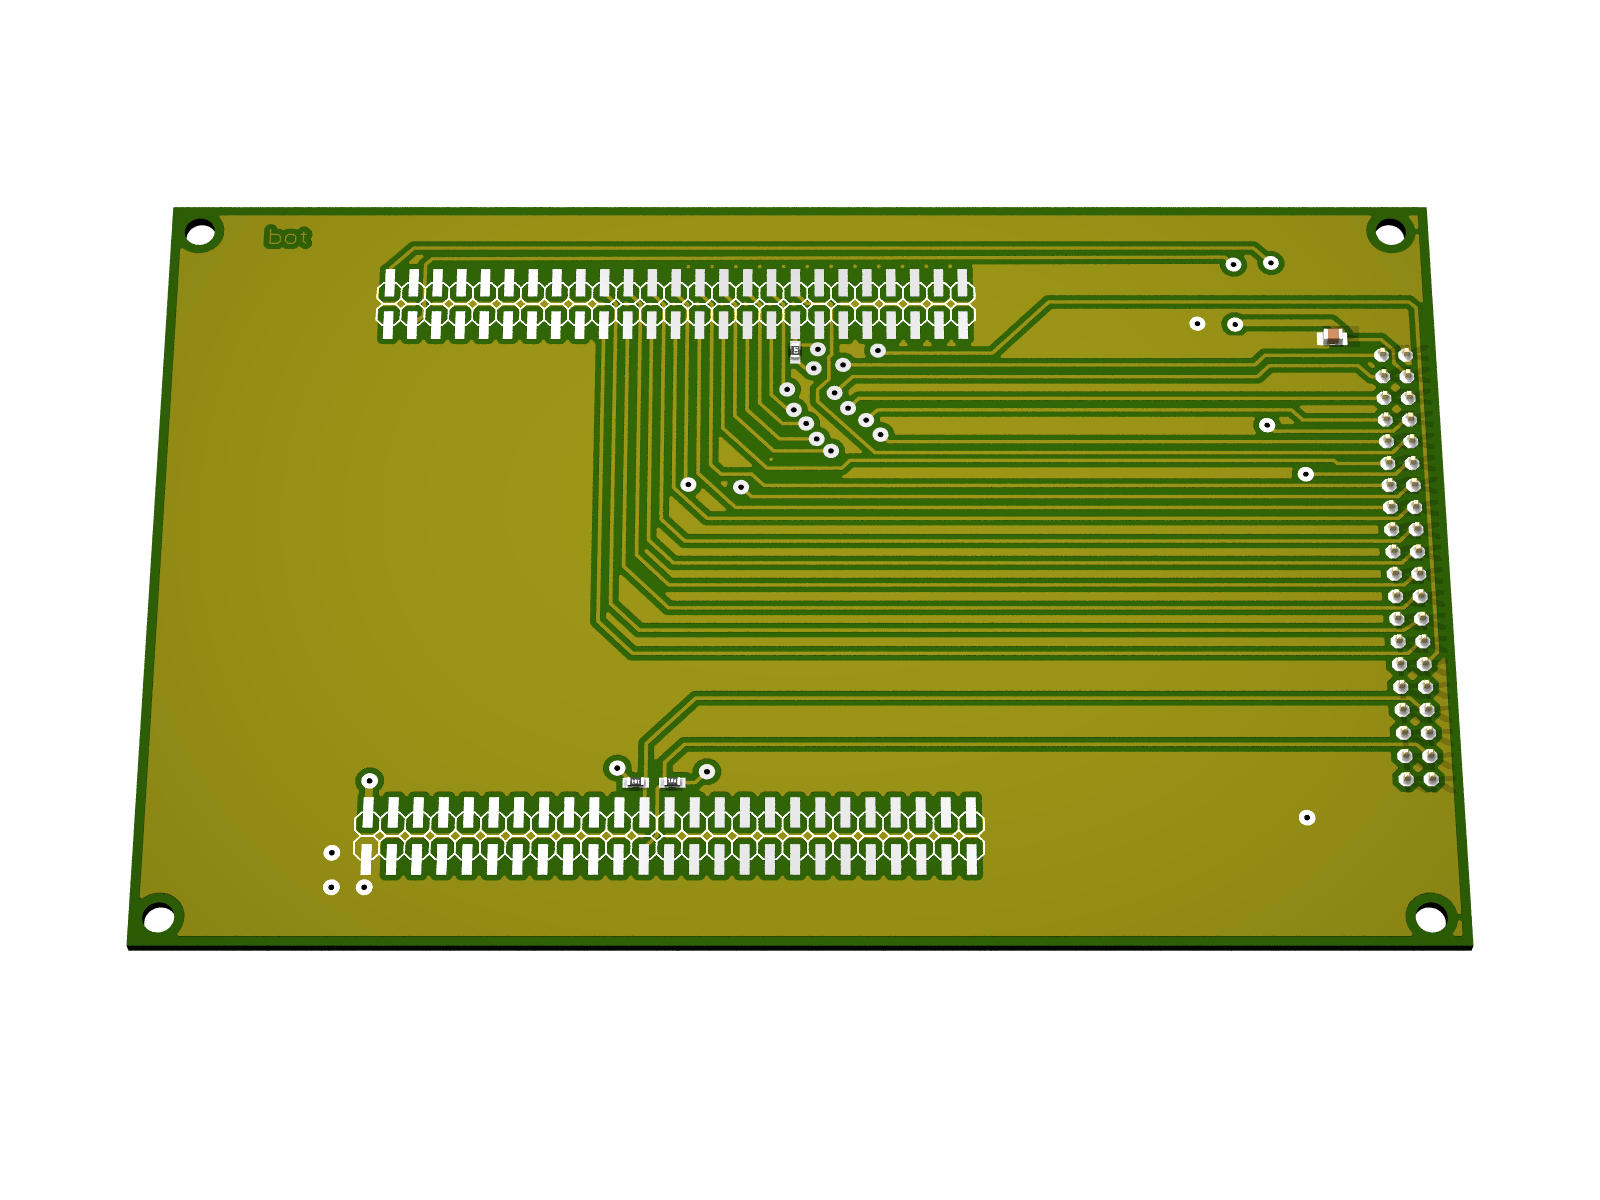
\includegraphics[width=\textwidth]{TeilA/gnublin_ext_ssd1963_bot.png} }              				\caption{Adapterplatine Bottom Layer}
                \label{fig:adapter_bot}
        \end{subfigure}
		\end{center}
        \caption{Adapterplatine zwischen Gnublin Extended und Display}\label{fig:adapterplatine}
\end{figure}

Die Schaltplan und das Layout befinden sich in der CD im Anhang dieser Arbeit.
\newpage
\subsection{Software}
Im Folgenden Abschnitt wird die Software behandelt, die nötig ist, um das Display zu betreiben. 
Die Softwareentwicklung ist in drei Teile auf gegliedert:
\begin{itemize}
\item Modifikationen im Bootloader APEX
\item Userspace-Treiber basierend auf einem Treibers auf für den Raspberry Pi (siehe \cite{Schlegel2013a} und \cite{Schlegel2013b}) bei dem mittels GPIO-Pins ein 8080-Display zu betreiben
\item Framebuffer-Treiber im Linux-Kernel
\end{itemize}

\subsubsection{Anpassung des APEX-Bootloaders zur Verwendung des Displays}
Der APEX-Bootloader\footnote{\url{https://gitorious.org/apex/}} wurde ursprünglich für Prozessoren de Sharp LH Familie entwickelt, wurde allerdings auf eine Vielzahl von weiteren ARM basierten Prozessoren portiert, so auch für die verwendete NXP LPC313x CPU\footnote{CPU: Central Processing Unit, Prozessor}.
Die Aufgabe des Bootloaders ist es, grundlegende prozessorinterne Hardwareeinheiten wie z.B. CGU oder SD-RAM zu initialisieren um für den Linux-Kernel die notwendige Umgebung zu schaffen. Im Anschluss wird der Linux-Kernel geladen und gestartet. Es werden außerdem dem Linux-Kernel Bootparameter übergeben, die zum Start benötigt werden. Am Anfang des Bootloader-Codes werden die verwendeten MPMC-Register konfiguriert. Wie in \refc{cha:mpmc} muss das SYSCREG-Register SYSCREG\_AHB\_MPMC\_MISC nicht explizit beschrieben werden, da es im Resetzustand bereits richtig konfiguriert ist. \refl{lst:apex_mpmc_config} zeigt die entsprechende Initialisierung der MPMC-Register für das MD050SD. Die Adressen von z.B. MPMC\_STCONFIG0 sind in der \lstinline|lpc313x.h| definiert. Die Modifikationen im Bootloader finden in der Datei \lstinline|initialize.c| statt.

\begin{lstlisting}[%
language=MyC,
caption={Bootloader: MPMC-Konfiguration},
label=lst:apex_mpmc_config
]
#elif defined(CONFIG_MACH_EPLPC3131_V1)
#if defined(CONFIG_DISP_SSD1963)
	// ...
#elif defined(CONFIG_DISP_MD050SD)
   /* LCD display, 16 bit */
   MPMC_STCONFIG0  = 0x81;
   MPMC_STWTWEN0   = 13;
   MPMC_STWTOEN0   = 0;
   MPMC_STWTRD0    = 0;
   MPMC_STWTPG0    = 0;
   MPMC_STWTWR0    = 15;
   MPMC_STWTTURN0  = 0;
#elif defined(CONFIG_DISP_SSD1289)
	// ...
#elif defined(CONFIG_DISP_NONE)
	// ...
#endif
#endif
\end{lstlisting}


\paragraph{Boot-Logo im APEX-Bootloader}
Um dem Display beim Systemstart einen initialisierten Zustand zu geben und dem Benutzer bereits während dem Laden des Linux-Kernels ein Bild anzuzeigen, ist ein Bootlogo konfigurierbar. Hierfür bedarf es eines rudimentären Displaytreibers im Bootloader. Im Folgenden wird die Darstellung des Boot-Logos unter Verwendung des MD050SD dargestellt. \refl{lst:apex_erster_teil} zeigt den ersten Teil des Treibers, bei dem grundlegende Datentypen sowie Sendefunktionen für Daten und Kommandos gelistet sind. 

\begin{lstlisting}[%
language=MyC,
caption={Bootloader: Grundlegende Datentypen und Funktionen},
label=lst:apex_erster_teil
]
#if defined(CONFIG_DISP_MD050SD) || defined(CONFIG_DISP_SSD1963) || defined(CONFIG_DISP_SSD1289)
#define DISP_PHYS        (EXT_SRAM0_PHYS)
#define DISP_PHYS_CTRL   (DISP_PHYS + 0)
#define DISP_PHYS_DATA   (DISP_PHYS + 0x10000)

unsigned int width;
unsigned int height;
int pixel;

struct display {
   volatile u16* ctrl;
   volatile u16* data;
};

static struct display display;

static void display_send_cmd(u16 cmd)
{
   *display.ctrl = 0x00FF & cmd;
}

static void display_send_data(u16 data)
{
   *display.data = data;
}

#endif
\end{lstlisting}

Die Struktur \lstinline|struct display| ab Zeile 10 von \refl{lst:apex_erster_teil} enthält zwei Zeiger \lstinline|u16* ctrl| und \lstinline|u16* data| auf die jeweiligen Adressen aus \reft{tab:sram_adressen} für Kommandos und Daten. In den Zeilen 17 und 22 sind die zwei Sendefunktionen \lstinline|display_send_cmd(u16 cmd)| und 
\lstinline|display_send_data(u16 cmd)| definiert. Hiermit werden die Kommandos und Daten an das Display gesendet. Wird auf eine der beiden Adressen ein Wert geschrieben, kümmert sich das MPMC und das EBI automatisch um die restlichen Signale wie WR, RD und CS. 

\begin{lstlisting}[%
language=MyC,
caption={Bootloader: Display-Initialisierung und Bootlogo},
label=lst:apex_zweiter_teil
]
#if defined(CONFIG_DISP_MD050SD) || defined(CONFIG_DISP_SSD1963) || defined(CONFIG_DISP_SSD1289)
   display.ctrl = &__REG16 (DISP_PHYS_CTRL);   
   display.data = &__REG16 (DISP_PHYS_DATA); 
#if defined(CONFIG_DISP_MD050SD)
   GPIO_OUT_LOW(IOCONF_GPIO, _BIT(14)); //GPIO20 is LED_ENABLE

   GPIO_OUT_LOW(IOCONF_GPIO, _BIT(13)); //GPIO19 is nRESET
   udelay(20000);
   GPIO_OUT_HIGH(IOCONF_GPIO, _BIT(13)); //GPIO19 is nRESET
   udelay(20000);

	/* Set Window from 0,0 to 479, 799 */
   display_send_cmd(0x0002);			
   display_send_data(0);				
   display_send_cmd(0x0003);			
   display_send_data(0);				

   display_send_cmd(0x0006);
   display_send_data(480 - 1);
   display_send_cmd(0x0007);
   display_send_data(800 - 1);

	/* Clear the display with color black */
   display_send_cmd(0x000F);

   for(pixel = 0; pixel < 800 * 480; pixel++)
   {
      display_send_data(0x0000);
   }

   GPIO_OUT_HIGH(IOCONF_GPIO, _BIT(14)); //GPIO20 is LED_ENABLE

#if defined(CONFIG_LOGO_TUX)
   width = boot_logo_tux[0];
   height = boot_logo_tux[1];

   display_send_cmd(0x0002);
   display_send_data(480/2 - (height - 1)/2);
   display_send_cmd(0x0003);
   display_send_data(800/2 - (width - 1)/2);
   display_send_cmd(0x0006);
   display_send_data(480/2 + (height - 1)/2 + 1);
   display_send_cmd(0x0007);
   display_send_data(800/2 + (width - 1)/2 + 1);
   display_send_cmd(0x000F);

   for(pixel = 2; pixel < width * height + 2; pixel++)
   {
      display_send_data(boot_logo_tux[pixel]);
   }
#endif
#endif
#endif
\end{lstlisting}

Der Eigentliche Treiber und der Code für das Anzeigen des Bootlogos ist in \refl{lst:apex_zweiter_teil} zu sehen. In Zeile 2 und 3 werden den Adresszeigern die pysikalischen Adressen zum Schreiben von Kommandos und Daten zugewiesen. Von Zeile 5 bis 10 wird die Hintergrundbeleuchtung explizit abgschaltet und ein Reset auf das Display gegeben. Da das MD050SD einen CPLD-Controller besitzt, welcher eine auf genau dieses TFT-Panel zugeschnittene Programmierung enthält, fällt eine Initialisierungsroutine weg. Dies wäre bei Controllern wie dem SSD1963 nicht der Fall, da diese mit einer Vielzahl von Panels arbeiten können und demzufolge eine spezielle Initialisierung brauchen. Das MD050SD ist nach dem Reset also initialisiert und erwartet Kommandos. Von Zeile 13 bis 24 in \refl{lst:apex_zweiter_teil} wird ein Bereich im Display-RAM der vollen Bildschirmgröße reserviert und die Bereitschaft zum Datenempfang gestartet (siehe \reft{tab:Kommandos_MD050SD}). Alle Daten die im Anschluss gesendet werden, werden automatisch an die richtige Stelle im Display geschrieben. In einer Schleife werden ab Zeile 26 alle reservierten Pixel von zuvor mit der Farbe Schwarz beschrieben, um das automatisch angezeigte Testbild des Displays beim Start zu überschreiben. Im Anschluss wird die Hintergrundbeleuchtung wieder eingeschaltet. Ist über den Codeswitch \lstinline|CONFIG_LOGO_TUX| das Bootlogo aktiviert, so wird dies ab Zeile 34 angezeigt. Die Größe des Logos wird in den Zeilen 34 und 35 ausgelesen und in den Folgenden angezeigt. Die Pixeldaten des Logos sind im Array \lstinline|u16 boot_logo_tux[]| in den Dateien \lstinline|boot_logo_tux.c| und \lstinline|boot_logo_tux.h| hinterlegt.


\paragraph{Konfiguration des APEX-Bootloaders}
Der APEX-Bootloader besitzt zur Konfiguration dasselbe System wie der Linux-Kernel. Dieses System heißt KConfig und wird durch den Befehl \lstinline|make menuconfig| aufgerufen, welches ein Konfigurationsmenü im aufrufenden Terminal erscheinen lässt. Hier sind neben Grundlegenden Konfiguration zum Beispiel für die Prozessorarchitektur oder Taktraten auch der Displaytreiber und das Bootlogo eingepflegt. \refa{fig:apex_config} zeigt exemplarisch den Unterpunkt \lstinline|Platform Setup| bei dem das Display MD050SD und das Bootlogo ausgewählt sind. 

\begin{figure}[tbph]
%\begin{figure}[h!]
	\centering
\fbox{	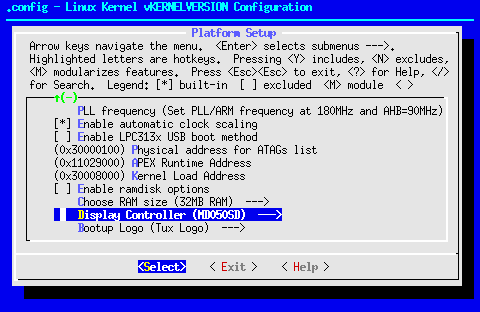
\includegraphics[width=0.8\textwidth]{TeilA/apex_config.png}}
	\caption{APEX-Bootloader KConfig}
	\label{fig:apex_config}
\end{figure}
\newpage

Bevor der Bootloader konfiguriert werden kann, muss der Vanilla-Quellcode noch gepatcht werden. \refl{lst:apex_patchen} zeigt die einzelnen Schritte, um den Bootloader herunterzuladen und zu Patchen. Der Patch enthält alle nötigen Dinge zum Betrieb des MD050SD-Display und des Boot-Logos.


\begin{lstlisting}[%
language=bash,
caption={Bootloader: Herunterladen und Patchen},
label=lst:apex_patchen
]
$ wget https://github.com/embeddedprojects/gnublin-distribution/raw/master/lpc3131/bootloader/apex/1.6.8/apex-1.6.8.tar.gz
$ tar xvfz apex-1.6.8.tar.gz
$ wget https://github.com/siredmar/master/raw/master/Teil_A/software/bootloader/apex_display.patch
$ cd apex-1.6.8
$ patch -p1 < ../apex_display.patch
\end{lstlisting}

Im Folgenden wird die Konfiguration des Bootloaders und die damit möglichen Einstellungsmöglichkeiten beschrieben. Im Konfigurationsmenü sind nach dem patchen im Untermenü \lstinline|Platform Setup| die Optionen \lstinline|Display Controller| und \lstinline|Bootup Logo| verfügbar. Hier wird die Auswahl bezüglich Displaycontrollers und Logo getroffen. Wird ein Displaycontroller anders als MD050SD gewählt, so werden nur entsprechende Timings der MPMC-Register gesetzt und kein Boot-Logo angezeigt. 
Um den Kernel mit spezifischen Parametern starten zu können, werden für den Betrieb der unterschiedlichen Treiber (Framebuffer, User-Space) andere Bootparameter benötigt. So ist der originalen Parameterliste 
\lstinline{console=ttyS0,115200n8 root=/dev/mmcblk0p3 rw rootfstype=ext4 rootwait} im Untermenü \lstinline|Environment| für den Betrieb mit dem Framebuffer-Treiber ein \lstinline|fbcon=rotate:0 fbcon=font:VGA8x16| hinzuzufügen um dem Kernel beim Start Informationen über den Kernel-Treiber \lstinline|fbcon| mitzuteilen. Wird der User-Space-Treiber verwendet, so übernimmt das Kernel-Modul \lstinline|vfb|\footnote{vfb: Virtual Frame Buffer} die Aufgabe des Framebuffers. Die Parameterliste ist mit \lstinline|console=tty0 video=vfb: vfb_enable=1| zu ergänzen (siehe \cite{LinuxKernelFBCON}).

Der Bootloader wird per \lstinline|make apex.bin| kompiliert und mit \lstinline|dd if=src/arch-arm/rom/apex.bin of=/dev/sdXY| \footnote{/dev/sdXY: bezieht sich auf die Bootpartition auf der korrekten SD-Karte, z.b. /dev/sdb2} auf die SD-Karte des Gnublin geschrieben (siehe \cite{GnublinWiki2013}).

\subsubsection{Entwicklung eines Linux-Framebuffer-Treibers}
\todo{Kernel patchen}
In diesem Abschnitt wird die Entwicklung des Framebuffer-Treibers beschrieben. Der Framebuffer-System bietet eine Abstraktionsebene für die Grafikhardware. Es enthält einen Bildspeicher der Grafikhardware und bietet Applikationen Zugriff auf diesen, ohne jedoch Informationen über die letztendlich verwendete Hardware selbst auf Low-Level-Ebene haben zu müssen. Ein Framebuffer-Device erzeugt die Node \lstinline|/dev/fbX| mit der fortlaufenden Nummer X, beginnend bei Null, für jede Instanz eines Framebuffers. Jede grafische Anwendung in einem Linux-System benötigt eine Funktionalität, die den aktuellen Bildschirminhalt speichert und  Applikationen zugriff darauf gewährt. Dabei ist es im wesentlichen unwichtig, ob die Anzeige selbst durch Hardware beschleunigt oder sogar nur rein virtuell realisiert wird, da die Applikation auf die Schnittstelle in \lstinline|/dev/fbX| zugreift (siehe  \cite{LinuxKernelFB}).
Programme wie zum Beispiel der X11-Server, Video-Player, QT\footnote{QT: C++-Klassenbibliothek zur 2D-Darstellung}, SDL\footnote{SDL: Simple Direct Media Layer, Grafikbibliothek zur 2D-Darstellung} usw. können dieses System nutzen. Gerade für leistungsschwächere Systeme bietet es dahingehend dieselben Möglichkeiten Programme Anzuzeigen, wie für High-End-Systeme. Einzig die Art und Weise des Befüllens und Auslesens des Framebuffers unterscheidet die Leistungsfähigkeit einzelner Systeme. So können Systeme mit zusätzlichen Grafikeinheiten die speziell zum Berechnen von 3D-Daten mit zum Beispiel der 3D-Grafikbibliothek OpenGL\footnote{OpenGL: 3D Grafikbibliothek} den Framebuffer mit "'hochwertigeren"' Inhalten füllen, als ein System, das diese Möglichkeit nicht besitzt. Die Abstraktionsebene für die Applikation bleiben aber dieselben. 

Mit der Entwicklung eines Framebuffer-Treibers, sind alle Vorteile erschlossen, welche das Framebuffer-System bietet. Diese sind eine standardisierte Schnittstelle für Applikationen, sowie die Gewissheit, dass, sofern es die Rechenleistung zulässt, prinzipiell alle bereits existenten Programme und Inhalte angezeigt werden können.
In den folgenden Abschnitten, wird die Entwicklung des Framebuffer-Treibers für die drei verwendeten Displays dargelegt, mit Fokus auf das MD050SD. 
\paragraph{Framebuffer-Treiber für MD050SD}
In diesem Abschnitt wird die Funktionsweise des Framebuffer-Treibers für das MD050SD beschrieben. Auf ein Listing des kompletten Treibers wird an dieser Stelle bewusst verzichtet, sondern nur die elementaren Funktionen und Gedanken aufgezeigt.

Der Treiber arbeitet konform mit dem "'Platform Device"'- und "'Platform Driver"'-System im Linux-Kernel (siehe \cite{LinuxKernelPlatformDeviceDriver}). Mit dem Platform-Device-System wird ein Pseudo-Bus erzeugt, mit dem sich verschiedene Platform-Driver verbinden können. So können beispielsweise mehrere voneinander unabhängige Instanzen eines Treibers oder vieler verschiedener Treiber im System verfügbar sein. Beinhaltet ein System ein Platform-Device, so muss es dem Linux-Kernel bekannt gemacht werden. Hierzu wird die Struktur \lstinline|struct platform_device| verwendet, die in \refl{lst:struct_platform_device} gezeigt ist.

\begin{lstlisting}[%
language=MyC,
caption={Framebuffer: struct platform\_device},
label=lst:struct_platform_device
]
struct platform_device {
	const char	*name;
	u32		id;
	struct device	dev;
	u32		num_resources;
	struct resource	*resource;
};
\end{lstlisting}

In der Struktur in \refl{lst:struct_platform_device} sind Datentypen enthalten, die einen eindeutigen Namen des Devices \lstinline|const char *name|, sowie eine ID \lstinline|u32 id|  bestimmen, einen Parameter zur Struktur \lstinline|struct device|, sowie einen Zeiger zur Struktur \lstinline|strut resource|, die letztendlich die Hardware-Ressourcen darstellen. Für den Platform-Driver ist die Struktur \lstinline|struct platform_driver| in \refl{lst:struct_platform_driver} gegeben, die Funktionszeiger für den Betrieb des Treibers und eine Struktur \lstinline|struct device_driver| enthält, welche zur Zuordnung mit dem entsprechenden Platform-Device dient.
\begin{lstlisting}[%
language=MyC,
caption={Framebuffer: struct platform\_driver},
label=lst:struct_platform_driver
]
struct platform_driver {
	int (*probe)(struct platform_device *);
	int (*remove)(struct platform_device *);
	void (*shutdown)(struct platform_device *);
	int (*suspend)(struct platform_device *, pm_message_t state);
	int (*suspend_late)(struct platform_device *, pm_message_t state);
	int (*resume_early)(struct platform_device *);
	int (*resume)(struct platform_device *);
	struct device_driver driver;
};
\end{lstlisting}

Wie ein Platform-Device definiert wird, ist \refl{lst:register_platform_devices} zu entnehmen. Die Modifikationen sind im Quellcode der Start-Datei der Architektur \lstinline|linux-2.6.33-lpc313x/arch/arm/mach-lpc313x/ea313x.c| eingepflegt. In den Zeilen 2 bis 13 wird die Ressource \lstinline|struct resource mdsd_resource[]| definiert, die zwei Einträge enthält. Hier werden die physikalischen Adressen für Kommandos und Daten  für das Display auf SRAM-Interface eingestellt, die der Platform-Driver verwenden wird. Die Struktur \lstinline|struct platform_device md050sd_device| wird ab Zeile 15 definiert, und enthaelt einen eindeutigen Namen "'m050sd"'. Dieser Name wird im Folgenden vom Platform-Driver ebenfalls verwendet, um eine Zuordnung zwischen Device und Driver zu ermöglichen.
In Zeile 22 ist die Funktion definiert, die letzendlich dem Linux-Kernel die Stuktur \lstinline|struct platform_device md050sd_device| übergibt, und das Platform-Device im System registriert. 
\begin{lstlisting}[%
language=MyC,
caption={Framebuffer: Plattform Device definieren},
label=lst:register_platform_devices
]
#if defined (CONFIG_FB_MD050SD)
static struct resource md050sd_resource[] = {
  [0] = {
     .start = EXT_SRAM0_PHYS + 0x00000 + 0x0000,
     .end   = EXT_SRAM0_PHYS + 0x00000 + 0xffff,
     .flags = IORESOURCE_MEM,
  },
  [1] = {
     .start = EXT_SRAM0_PHYS + 0x10000 + 0x0000,
     .end   = EXT_SRAM0_PHYS + 0x10000 + 0xffff,
     .flags = IORESOURCE_MEM,
  },
};

static struct platform_device md050sd_device = {
  .name          = "md050sd",
  .id            = 0,
  .num_resources = ARRAY_SIZE(md050sd_resource),
  .resource      = md050sd_resource,
};

static void __init ea_add_device_md050sd(void)
{
  // ...
  platform_device_register(&md050sd_device);
  // ...
}
#else
static void __init ea_add_device_md050sd(void) {}
#endif /* CONFIG_FB_MD050SD */
\end{lstlisting}
Der Aufruf, der die Registrierung anstößt ist in \refl{lst:add_platform_devices} zu sehen. In der Funktion \lstinline|void __init ea313x_init(void)| werden alle Hardwareeinheiten, die vom Bootloader noch nicht konfiguriert wurden initialisiert und die verwendeten Devices im System registriert. Ohne eine vorhergehende Registrierung ist ein Verwenden eines Treibers nicht möglich.

\begin{lstlisting}[%
language=MyC,
caption={Framebuffer: Platform Devices im System registrieren},
label=lst:add_platform_devices
]
static void __init ea313x_init(void)
{
	lpc313x_init();
	platform_add_devices(devices, ARRAY_SIZE(devices));
    // ...
	ea_add_device_ssd1963();
	ea_add_device_ssd1289();
	ea_add_device_md050sd();
	// ...
}
\end{lstlisting}

In der Datei \lstinline|linux-2.6.33-lpc313x/drivers/video/md050sd.c| befindet sich der Displaytreiber selbst. Analog zu \refl{lst:struct_platform_driver} wird in \refl{lst:set_platform_driver} die Struktur instanziiert und die nötigen Funktionszeiger und der Name des Treibers eingesetzt. Hier wird derselbe Name genutzt, der bereits für das Platform-Device verwendet wurde. Nachdem der Treiber initialisiert wurde, wird dieser mit dem Pseudo-Bus verbunden. Der Linux-Kernel ist nun in der Lage dem Treiber die vorher definierten Ressourcen zu übergeben.

\begin{lstlisting}[%
language=MyC,
caption={Framebuffer: Platform Driver},
label=lst:set_platform_driver
]
static struct platform_driver md050sd_driver = {
      .probe = md050sd_probe,
      .remove = md050sd_remove,
      .driver = {
            .name = "md050sd",
      },
};
\end{lstlisting}

Wird der Treiber geladen, ob als Modul oder fest in den Kernel kompiliert, wird die Funktion aufgerufen, die im Makro \lstinline|module_init()| definiert ist. So wird die Funktion \lstinline|static int __init md050sd_init(struct patform_deice *dev)| aufgerufen, die den Platform-Driver mit der zuvor definierten Struktur \lstinline|md050sd_driver| aus \refl{lst:set_platform_driver} im Linux-Kernel mittels 
\lstinline|platform_driver_register(&md050sd_driver)|  \todo{line break fixen!} registriert. Die Funktion \lstinline|md050sd_probe()| ist in \refl{lst:probe_funktion} zu sehen. 
Nach der Registrierung wird der Treiber geladen. Hier wird die Probe-Funktion \lstinline|md050sd_probe()| aufgerufen, die zuerst den benötigten Speicher für den Treiber selbst alloziert, die Zeiger für Kommandos und Daten aus der IO-Ressource des platform\_device holt, den Speicher für den Framebuffer alloziert und diesen mit entsprechenden Werten füllt. Im Anschluss wird ein initiales Update des Bildschirms vollzogen, dass das aktuelle Bild auf dem Display löscht. Zur besseren Lesbarkeit, wurde die komplette Fehlerbehandlung aus dem Listing entfernt. 

\begin{lstlisting}[%
language=MyC,
caption={Framebuffer: Probe-Funktion},
label=lst:probe_funktion
]
static int __init md050sd_probe(struct platform_device *dev)
{
   int ret = 0;
   struct md050sd *item;
   struct resource *ctrl_res;
   struct resource *data_res;
   unsigned int ctrl_res_size;
   unsigned int data_res_size;
   struct resource *ctrl_req;
   struct resource *data_req;
   struct fb_info *info;
	// ... Allocate memory for driver
   item = kzalloc(sizeof(struct md050sd), GFP_KERNEL);
   item->dev = &dev->dev;
   dev_set_drvdata(&dev->dev, item);
   item->backlight = 1;
   // ... Get ctrl addresses from platform_device IORESOURCE
   ctrl_res = platform_get_resource(dev, IORESOURCE_MEM, 0);
   ctrl_res_size = ctrl_res->end - ctrl_res->start + 1;
   ctrl_req = request_mem_region(ctrl_res->start, ctrl_res_size,
         dev->name);
   item->ctrl_io = ioremap(ctrl_res->start, ctrl_res_size);
   // ... Get data addresses from platform_device IORESOURCE
   data_res = platform_get_resource(dev, IORESOURCE_MEM, 1);
   data_res_size = data_res->end - data_res->start + 1;
   data_req = request_mem_region(data_res->start,
         data_res_size, dev->name);
   item->data_io = ioremap(data_res->start, data_res_size);
   // ... Allocate Framebuffer Memory and fill it with logic
   info = framebuffer_alloc(sizeof(struct md050sd), &dev->dev);
   // ... Set framebuffer specific stuff
   info->pseudo_palette = &item->pseudo_palette;
   item->info = info;
   info->par = item;
   info->dev = &dev->dev;
   info->fbops = &md050sd_fbops;
   info->flags = FBINFO_FLAG_DEFAULT | FBINFO_VIRTFB;
   info->fix = md050sd_fix;
   info->var = md050sd_var;
   ret = md050sd_video_alloc(item);
   info->screen_base = (char __iomem *) item->info->fix.smem_start;
   ret = md050sd_pages_alloc(item);
   // ... Set Deferred IO settings to framebuffer
   info->fbdefio = &md050sd_defio;
   fb_deferred_io_init(info);
   ret = register_framebuffer(info);
   // ... initial screen update
   md050sd_setup(item);
   md050sd_update_all(item);
   // ...
   return ret;
}
\end{lstlisting}

\paragraph{Anpassungen für SSD1963 Controller}
\paragraph{Anpassungen für SSD1289 Controller}

\subsubsection{Entwicklung eines User-Space-Treibers}
\paragraph{Anpassungen für SSD1963 Controller}
\paragraph{Anpassungen für SSD1289 Controller}
\paragraph{Anpassungen für MD050SD}
\subsubsection{Probleme bei der Entwicklung und Fehlersuche}
\paragraph{Probleme mit SSD1963}
\subparagraph{Rolle des User-Space-Treibers}
\subparagraph{Debuggen mit Logik-Analyzer}





% \section{Vor- und Nachteile}
\section{Known Bugs}
Im Laufe der Entwicklung gab es Erschwernisse, welche die Entwicklung verzögerten. 
Als Einschränkung bezüglich des MD050SD, stellt sich die begrenzte Geschwindigkeit von 50~MHz dar. Mit einer maximalen Busgeschwindigkeit von 90~MHz, könnte das Display wesentlich schneller betrieben werden, was die Framerate fast verdoppeln würde. Zusätzlich erscheinen auf dem Display zufällig Artefakte in Form von einzelnen Pixeln, was die Vermutung zulässt, dass die Leitungen von der Adapterplatine oder des MD050SD selbst anfällig für Störungen von außen sein können. \\ \\
Bezüglich dem SSD1289 stellte sich heraus, dass die Verwendung der angebotenen Kommandos aus \reft{tab:Kommandos_SSD1289} nicht für die Adressierung eines RAM-Fensters über mehrere Zeilen zuverlässig funktioniert. Unabhängig vom gesendeten Kommando treten hier zufällige Resets des Displaycontrollers auf, welche das Display nach kurzer Zeit komplett weiß erscheinen lässt. Als Lösung stellte sich die Reservierung einzelner Zeilen dar, die in der Summe das komplette RAM-Fenster abdecken. Nachteilig stellt sich hierbei der erhöhte Adressierungsaufwand dar, da jede Zeile erneut adressiert werden muss.\\ \\
Der Betrieb mit dem SSD1963 stellt sich problematischer dar, als anfangs angenommen. Die Ursache des Problems ist noch ungeklärt, was den Betrieb mit dem SSD1963 derzeit unmöglich macht.
Das Problem stellt sich so dar, dass sich trotz scheinbar korrektem Datenverkehr auf dem 8080-Bus der Displaycontroller nicht initialisieren lässt. Als erster Schritt steht immer die PLL\footnote{PLL: Phase Locked Loop, Phasenregelschleife zur Erzeugung von hohen Taktraten}. Mithilfe der PLL wird der erforderliche Displaytakt von z.~B. 90~MHz erzeugt und der Controller mit dieser Frequenz betrieben. Ein solche schneller Zugriff auf den SSD1963 ist erst nach der Initialisierung der PLL möglich. Bevor dies der Fall ist, kann mit maximal 5 M Words/s \footnote{5M~Word/s: $5*10^6$ Datenwörter pro Sekunde} geschriebenen bzw. gelesen werden (siehe \cite{SSD2008}, S. 72). Der Fehler stellt sich so dar, dass sich die PLL nicht initialisieren lässt. Um den Fehler zu finden, wurden diverse Überlegungen vorangestellt. Angedachte potentielle Fehlerquellen sind
\begin{itemize}
\item zu flache Flanken der Signale
\item 8080-Bus Protokoll nicht eingehalten
\item 8080-Bus Timing nicht im Rahmen der Spezifikationen
\item 8080-Bus Datenverkehr fehlerhaft
\item Leitungsführung auf dem Display selbst schlecht
\end{itemize}
Die Flanken der Signale haben sich nach Messungen mit dem Oszilloskop als nicht zu flach herausgestellt und können als Fehlerquelle ausgeschlossen werden. Die Einhaltung des 8080-Bus Protokolls, samt der Einhaltung der Timings wurden ebenfalls überprüft. Hierzu ist dasselbe Display mit einer funktionierenden Displayansteuerung über die GPIO-Pins aufgebaut worden und jedes Kommando der Initialisierung des SSD1963 mit dem Logic-Analyzer aufgenommen worden. Derselbe Displaytreiber, mit dem Unterschied der Ansteuerung über das SRAM-Interface, wurde ebenfalls aufgezeichnet und mit den Daten der vorhergehenden Messung verglichen. Diese Methode schließt einen Fehlerhaften Datenverkehr aus und lässt zusätzlich die Rahmenbedingungen für das 8080-Interface selbst und dessen Timing überprüfen. Für die Aufzeichnung, wurde der User-Space-Treiber dahingehend modifiziert, dass er vor dem Senden die Bestätigung des Anwenders abfragt. Die Abbildungen \ref{fig:ssd1963_gpio} und \ref{fig:ssd1963_sram} zeigen einen exemplarischen Datentransfer für die beiden Ansteuerungsmethoden. Zu erkennen ist, dass dasselbe Wort an den Datenpins D[7:0] anliegt, und die Steuersignale CS, WR, RD und A15 entsprechend innerhalb der markierten Zonen entsprechend dem 8080-Interface geschaltet werden. 

\begin{figure}[htp]
        \begin{center}
        \begin{subfigure}[htp]{1\textwidth}
			%\begin{figure}[h!]
			\centering
			\fbox{	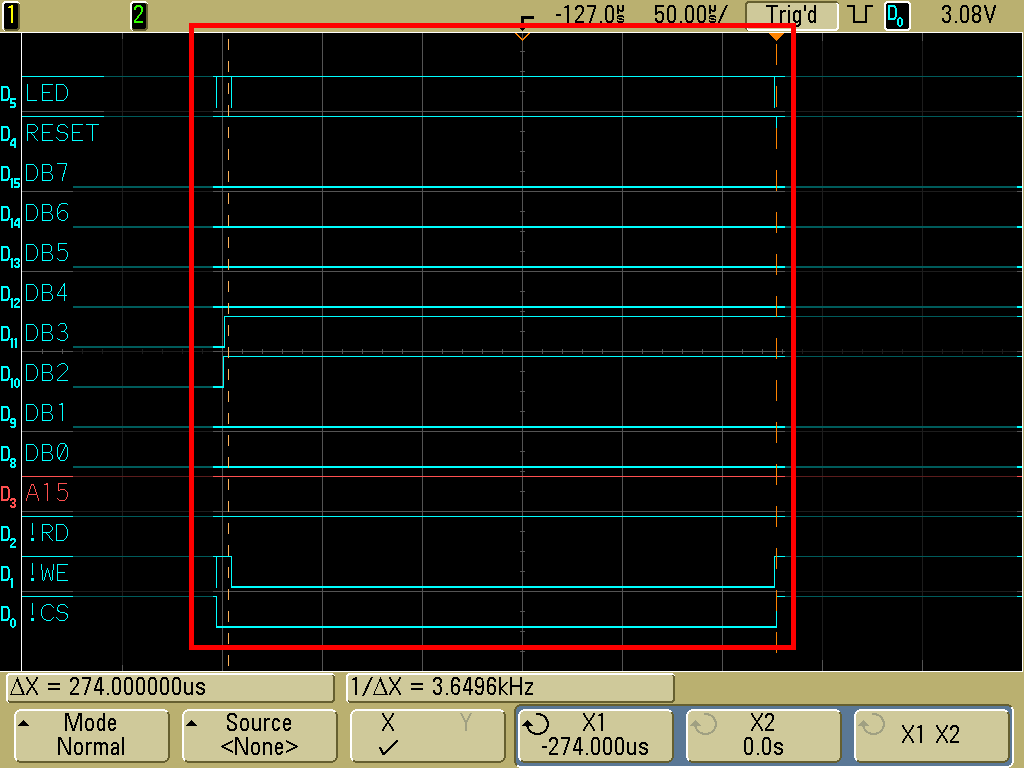
\includegraphics[width=1\textwidth]{TeilA/print_34_dip.png}}
	\caption{SSD1963 mit GPIO}
			\label{fig:ssd1963_gpio}
		\end{subfigure}


        \begin{subfigure}[htp]{1\textwidth}
%\begin{figure}[h!]
	\centering
\fbox{	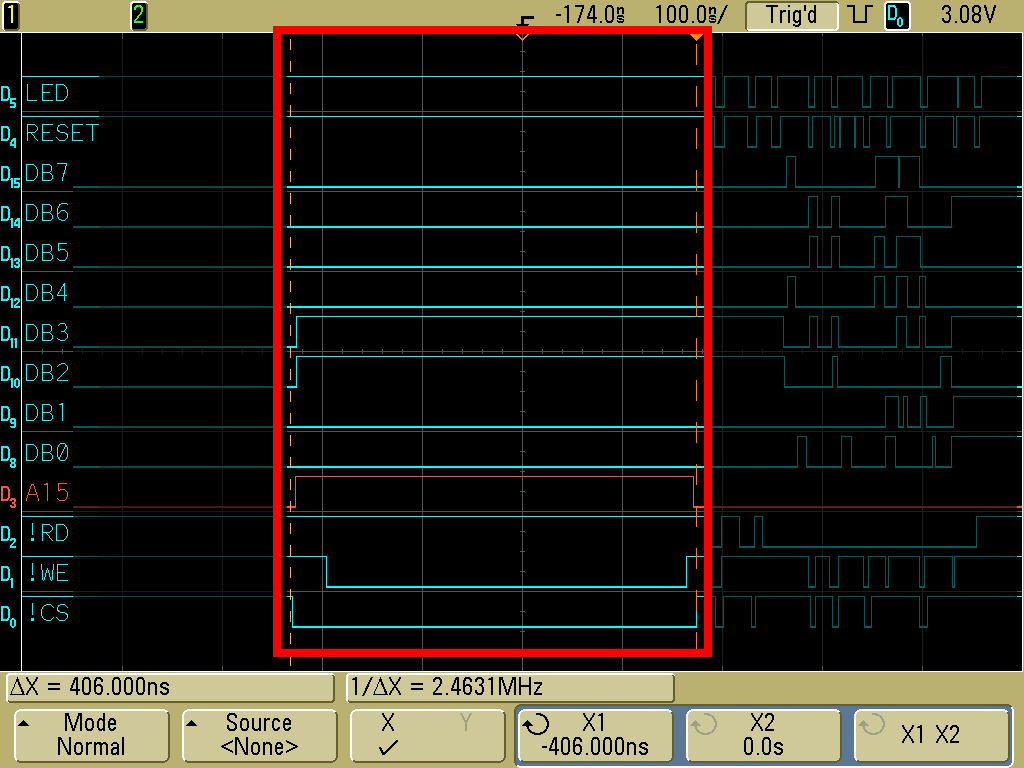
\includegraphics[width=1\textwidth]{TeilA/print_34_ext.png}}
	\caption{SSD1963 mit SRAM-Interface}
	\label{fig:ssd1963_sram}
\end{subfigure}

		\end{center}
\caption{SSD1963: Vergleich GPIO- und SRAM-Ansteuerung}
	\label{fig:ssd1963_gpio_sram}
\end{figure}
\newpage
Das geforderte Timing ist in \refa{fig:ssd1963_timing_constraints} zu sehen und beinhaltet die minimal notwendigen Zeiten zwischen den einzelnen Signalen.
\begin{figure}[htp]
%\begin{minipage}[t]{0.8\textwidth}
%\begin{figure}[h]
	\centering
\fbox{	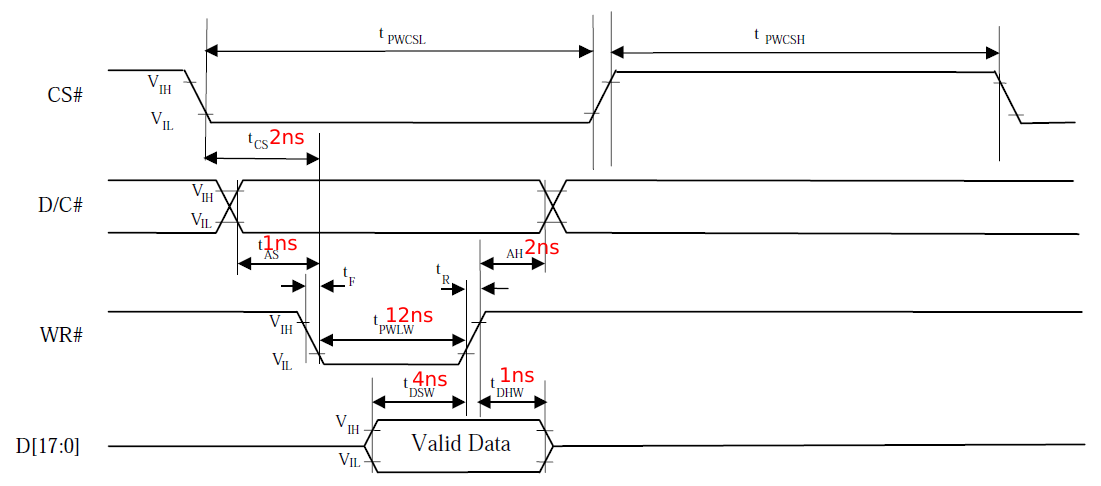
\includegraphics[width=1.0\textwidth]{TeilA/ssd1963_writeCycleConstraings.png}}
	\caption{8080-Timingbedingung für SSD1963}
	\label{fig:ssd1963_timing_constraints}
\end{figure}
Diese Mindestzeiten wurden innerhalb der Oszilloskopbilder eingehalten und verifiziert, sodass ein Fehler mit dem Protokoll des 8080-Interface ausgeschlossen werden kann. Bezüglich der uninitialisierten PLL des Displays und der verringerten Schreibrate ist in \refa{fig:ssd1963_sram} eine Chip-Select-Laenge von 406~Nanosekunden erkennbar, was einer Schreibgeschwindigkeit von 2.46~MHz entspricht. Dies ist weit unter den geforderten 5~MHz im uninitialisierten Zustand. Ein zu schnelles Schreiben ist in diesem Fall ebenfalls ausgeschlossen. Nachdem verifiziert wurde, dass aus der Adapterplatine vom Gnublin Extended die richtigen Signale geliefert werden, bleibt als Ursache nur noch das Display selbst. Da die Leitungsführung des ursprünglich verwendeten 4.3"' Displays nicht optimal ist, bei dem die 8080-Leitungen quer über die Platine geführt und im Anschluss von den RGB-Signalen im 90 Grad Winkel gekreuzt werden, wurde der Fehler im schlechten Platinendesign des Displays gesucht. Aufgrund dessen fand das 5"' Display mit demselben Controller Verwendung, das eine optimierte Leitungsführung besitzt. Jedoch waren die aufgeführten Lösungsansätze nicht zielführend, weswegen das Display nicht mit dem Gnublin Extended unter Verwendung des SRAM-Interface einsetzbar ist.

\input{Inhalt/TeilA/TeilAZusammenfassung}


\chapter{Teil B}
\label{cha:TeilB}
Im Folgenden wird Teil B dieser Arbeit behandelt. Bei embedded-Linux Systemen mit höherer Leistung und dedizierter Grafikhardware mit 3D-Beschleunigung oder Full-HD Anzeige, ist die Frage nicht, ob sondern eher welches Display angeschlossen werden kann. Die HDMI-Schnittstelle bietet bereits die Möglichkeit eine Vielzahl von Anzeigegeräten anzuschließen. Befindet man sich allerdings im embedded Bereich, so sind die Anforderungen an die Kompaktheit der Baugröße oft von sehr großer Bedeutung. Zu diesem Zweck wurde in Teil B dieser Arbeit eine Möglichkeit entwickelt, die den Anschluss von ausgewählten Displays mit einem Formfaktor von 7 Zoll bei der Auflösung von 800x480 mit RGB- sowie LVDS-Schnittstelle auf kompaktem Raum mit dem HDMI-Anschluss des embedded-Boards \code{Raspberry Pi} verbinden lässt. Betrachtet man die entwickelte Hardware näher, wird klar, dass diese mit jeder erdenklichen HDMI-Quelle verwendbar ist und im weitesten Sinne einen kompakten HDMI-Monitor darstellt.
In den nachfolgenden Kapiteln wird die Konzeption sowie die entwickelte Hard- und Software behandelt. Im Anschluss folgt ein Kapitel, welches die bekannten Fehler im Projekt aufzeigt.\newpage
\section{Konzept}
\label{sec:TeilB_Konzept}
Um die Entwicklung zielführend zu gestalten ist neben der Bauteilrecherche eine grobe Hardwarearchitektur zu erstellen, welche sich im Laufe immer mehr verfeinert. Die letztendliche Architektur wird als Ausgangspunkt für weitere Entwicklungen genommen. Treten Probleme während der Entwicklung auf, wie z. B. Bauteile können nicht geliefert/sind zu teuer oder gewünschte Bauform so nicht verfügbar, sind Alternativen zu finden, mit dem Ziel das Konzept bestenfalls nur minimal ändern zu müssen. Um solchen Problem aus dem Weg zu gehen, ist eine vollständiges Konzept sowie eine Bauteildatenbank inklusive Lieferdaten der Bauteile im Vorfeld zu erstellen. Das Projekt orientiert sich bezüglich der Konversion von HDMI nach RGB und LVDS an der Application Note SLLA325A von Texas Instruments (siehe \cite{TI2011}).
\begin{figure}[htp]
%\begin{minipage}[t]{0.8\textwidth}
%\begin{figure}[h]
	\centering
\fbox{	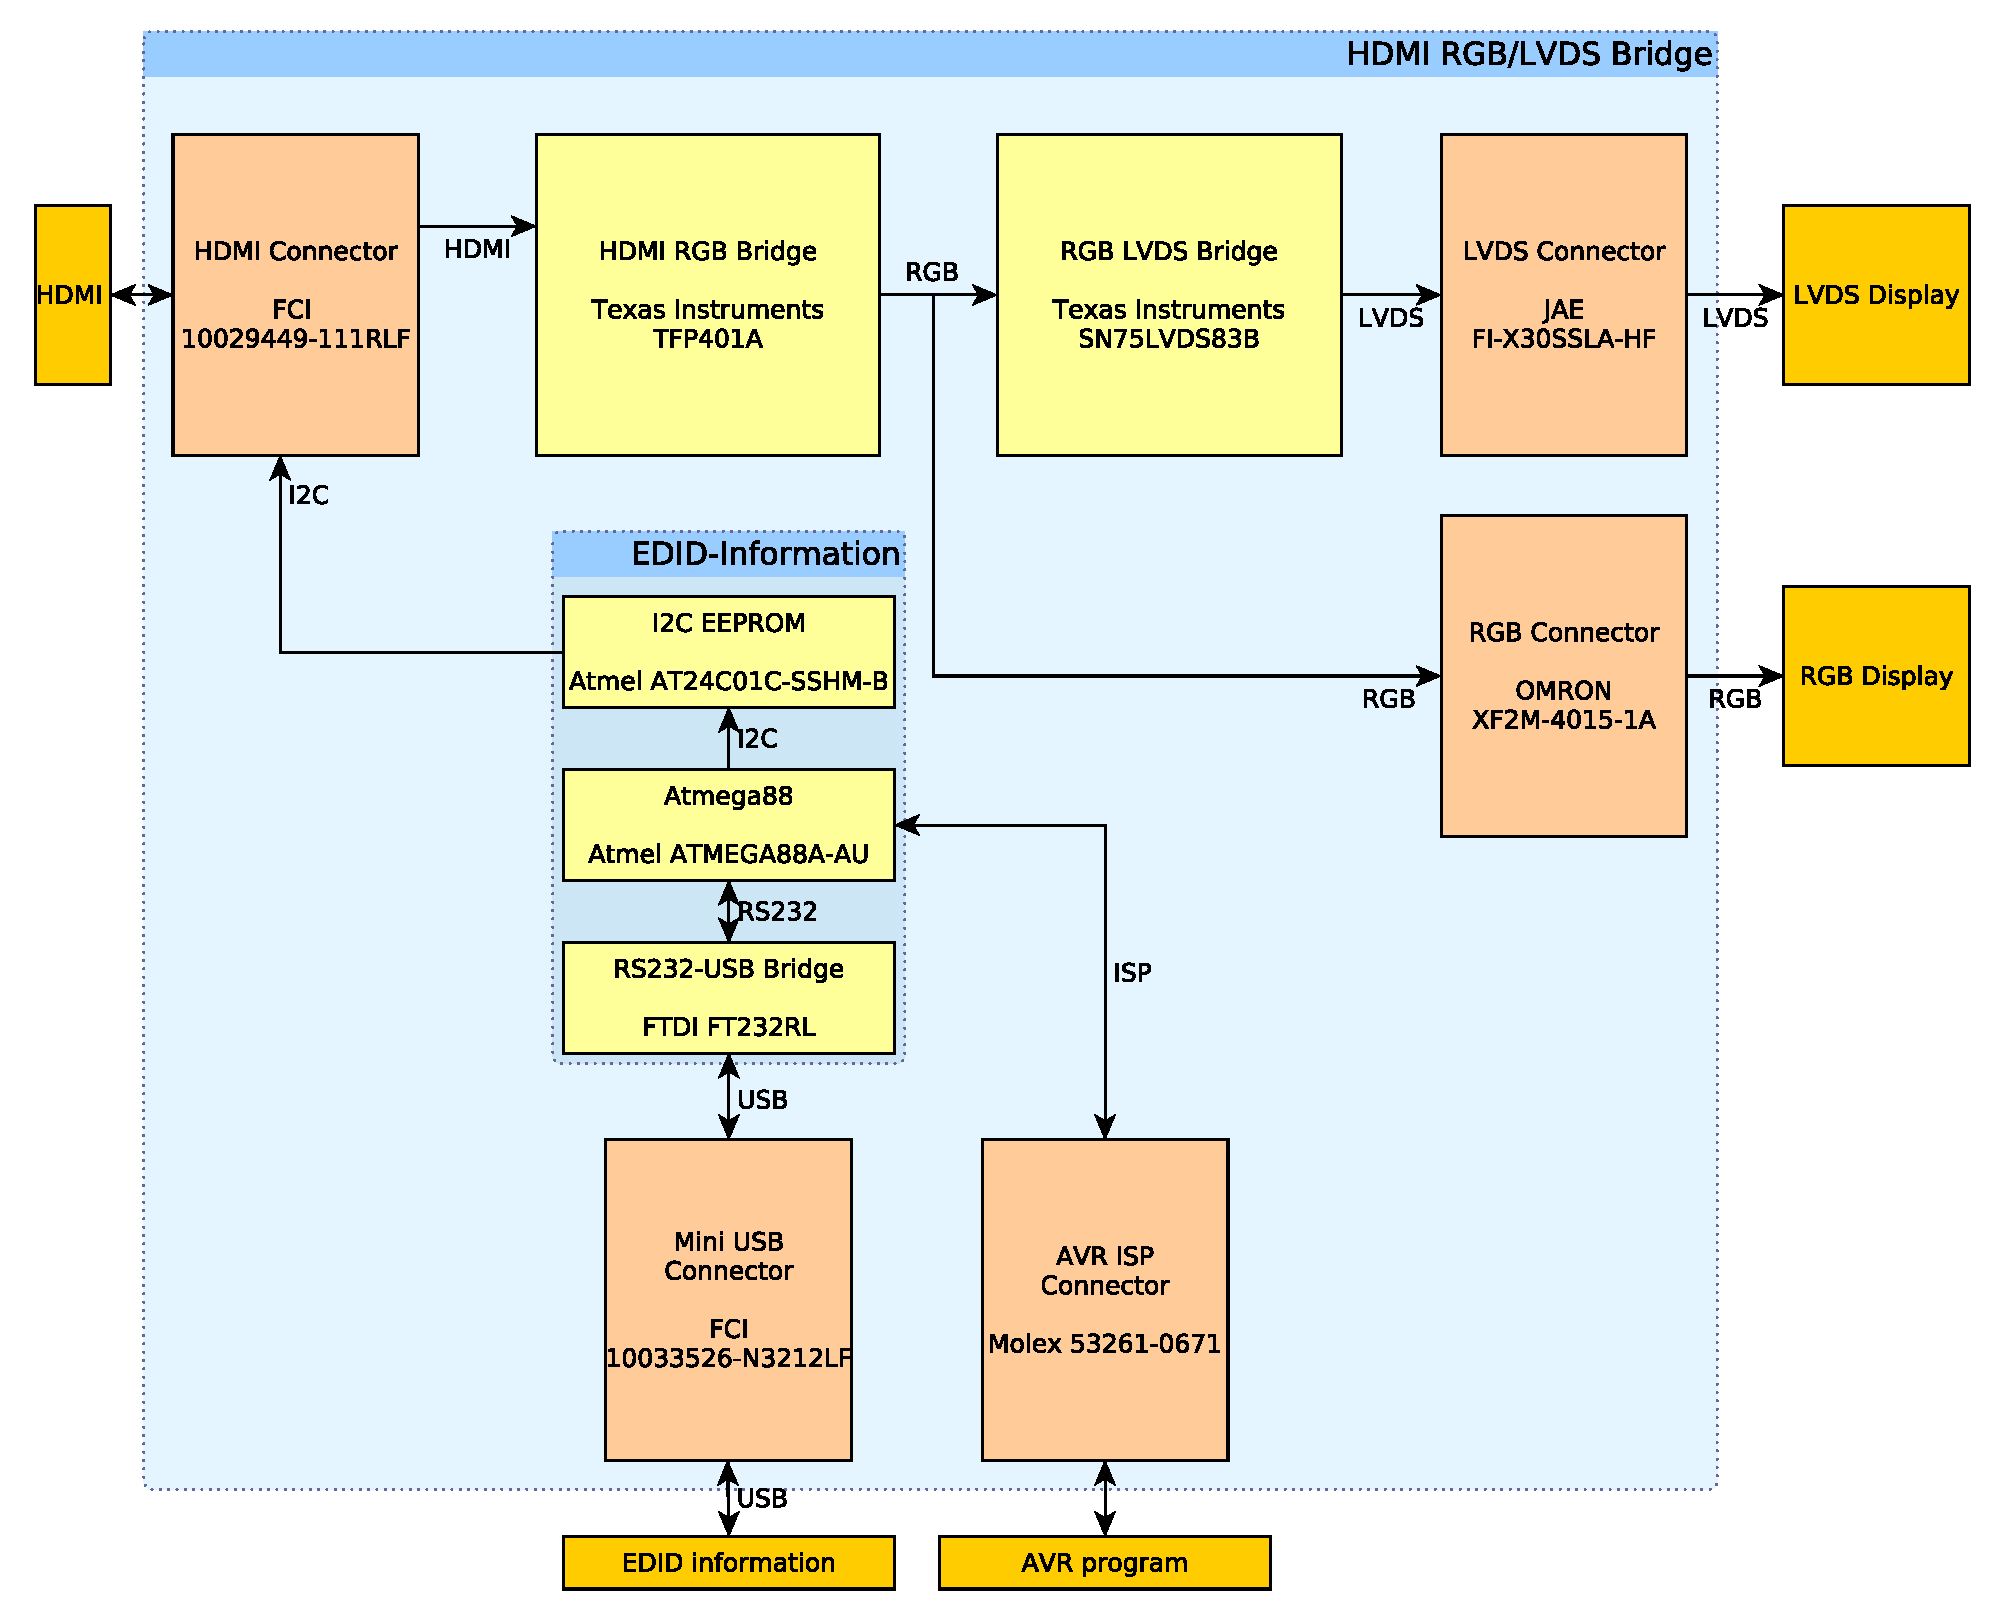
\includegraphics[width=1.0\textwidth]{TeilB/Architektur.pdf}}
	\caption{Hardware-Architektur}
	\label{fig:teilb_architektur}
\end{figure}

\refa{fig:teilb_architektur} zeigt die komplette Architektur des Projekts mit allen, für das Projekt notwendigen Eckpunkten und Verbindungen. So sind Schnittstellen nach Assen mit Rot markiert und die interne Logik mit Gelb. Als Signalquelle wird das HDMI-Signal eingespeist und in die HDMI-RGB-Bridge geleitet. Der Baustein \code{TFP401A} konvertiert die eingehenden HDMI-Signale auf den RGB-Bus. Hier kann direkt über einen FPC-Stecker\footnote{FPC: Fine Pitch Connector} ein RGB-Display anschlossen werden. Die Leitungen werden weitergeleitet zu einer RGB-LVDS-Bridge. Diese wandelt die RGB-Signale in LVDS-Signale entsprechend der benötigten Beschaltung des verwendeten Displays um. Verbindet man die Platine mit einer HDMI-Quelle, so tauschen diese Informationen aus und der Monitor sendet seine Leistungsfähigkeit bzgl. Auflösung, Timings, etc. an die Quelle. Diese Daten werden als EDID-Daten\footnote{EDID: Extended Display Identification Data} bezeichnet (siehe \cite{edid2010}). Gespeichert werden die EDID-Daten üblicherweise in einem EEPROM\footnote{EEPROM: Electrically Eraseable Programmable Read-Only Memory}, auf welches mit dem I2C-Bus zugegriffen werden kann. Um dieses EEPROM mit dem korrekten Inhalt beschreiben zu können, ist eine Baugruppe, in \refa{fig:teilb_architektur} mit dem Titel \code{EDID-Information} markiert, realisiert, welche über die USB-Schnittstelle nutzbar ist. Der USB-Seriell-Konverter FT232RL kommuniziert mit einem 8 Bit Atmel ATMega88 Prozessor, welcher das I2C-EEPROM direkt beschreiben kann. Um die korrenten EDID-Informationen in das EEPROM zu schreiben ist die zugehörige PC Software zu verwenden (siehe \refc{edid_pc}).\newpage
\section{Hardwareentwicklung}
\label{sec:TeilB_Hardware}
In diesem Kapitel wird auf die entwickelte Hardware eingegangen und detailliert dargestellt. Die Abbildungen \ref{fig:teilb_pcb_top} und \ref{fig:teilb_pcb_bot} zeigen die Ober- bzw. Unterseite der 4-lagigen Platine. In den Bildern sind farblich die einzelnen Bereiche der Platine markiert. Die Platine hat eine Größe von 70\,mm x 60\,mm.

\begin{table}[h]
\begin{tabular}{|p{8cm}|p{5.5cm}|}\hline
\rowcolor{TableBackgroundColor} 
   \textbf{Bereich auf Platine} & \textbf{Farbe}\\ \hline
  HDMI-Eingang &  \textcolor{red}{Rot} \\ \hline
  RGB-Bridge & \textcolor{yellow}{Gelb} \\ \hline
  LVDS-Bridge & \textcolor{blue}{Blau}  \\ \hline
  EDID-Daten &  \textcolor{orange}{Orange} \\ \hline
  Spannungsversorgung &  \textcolor{green}{Grün} \\ \hline 
\end{tabular}
\caption{Farblich gekennzeichnete Bereiche auf der Platine}
\label{tab:pcb_areas}
\end{table}

\begin{figure}[htbp]
        %\begin{center}
        \centering
        \begin{subfigure}[htp]{0.48\textwidth}
                \fbox{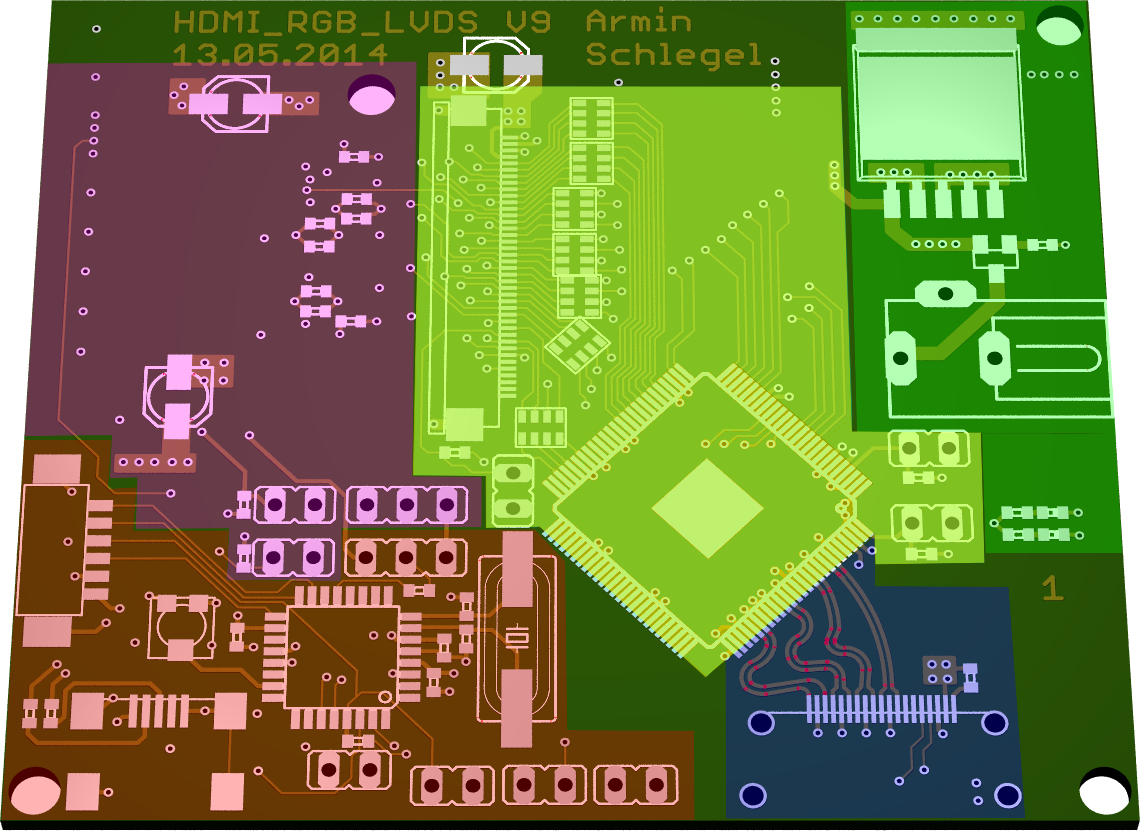
\includegraphics[height=4.7cm]{TeilB/HDMI_RGB_LVDS_V9_top.png}}
                \caption{Top Layer}
                \label{fig:teilb_pcb_top}
        \end{subfigure}
\quad 
        \begin{subfigure}[htp]{0.48\textwidth}
               \fbox{ 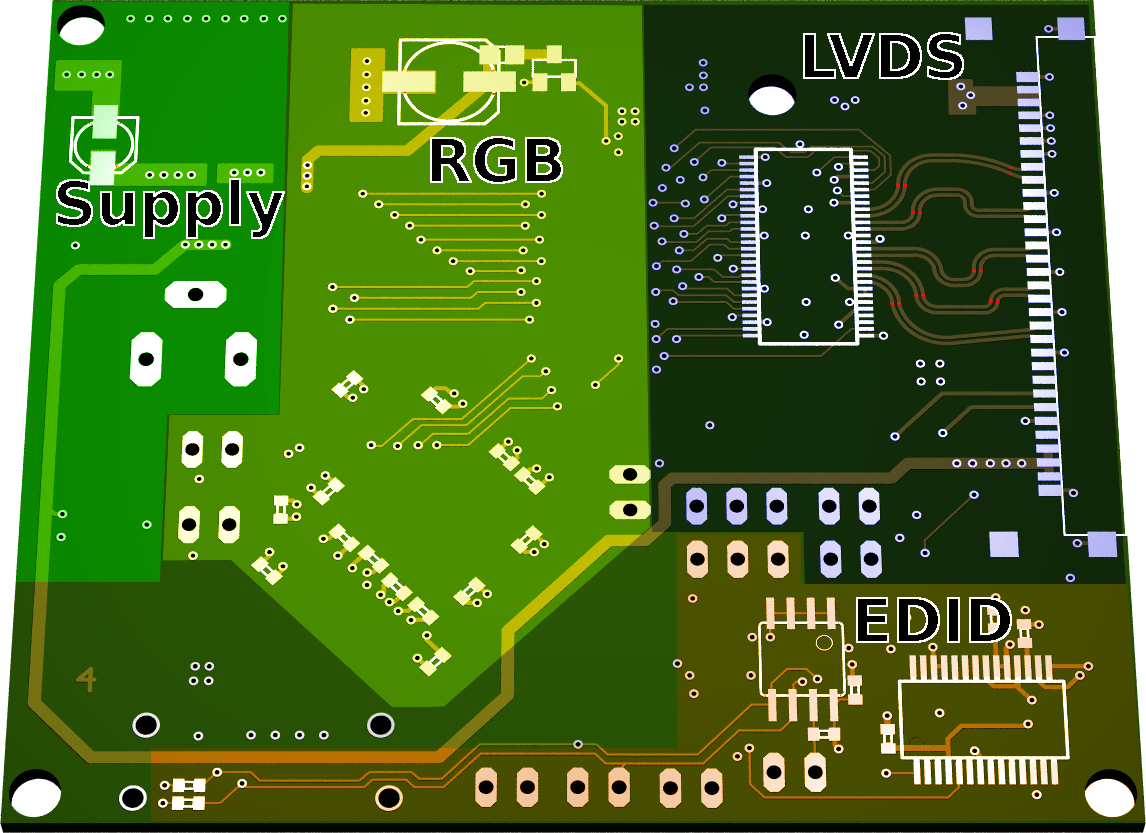
\includegraphics[height=4.7cm]{TeilB/HDMI_RGB_LVDS_V9_bot.png} }              				\caption{Bottom Layer}
                \label{fig:teilb_pcb_bot}
        \end{subfigure}
		%\end{center}
        \caption{HDMI RGB/LVDS Board}
        \label{fig:teilb_pcb}
\end{figure}

In den folgenden Abschnitten wird auf die Teilbereiche der Platine im Einzelnen eingegangen. Der Lagenaufbau ist entsprechend dem des Leiterplattenhersteller für vierlagige Platinen angelegt und ist in \refa{fig:teilb_lagenaufbau} zu sehen. Die Kupferdicke der einzelnen Lagen beträgt 35\,µm. Die beiden inneren Lagen sind als Versorgunglayer zur Leitung von Ground, +5\,V und +3.3\,V vorgesehen.
        \begin{figure}[htp]
        	\center
			\fbox{	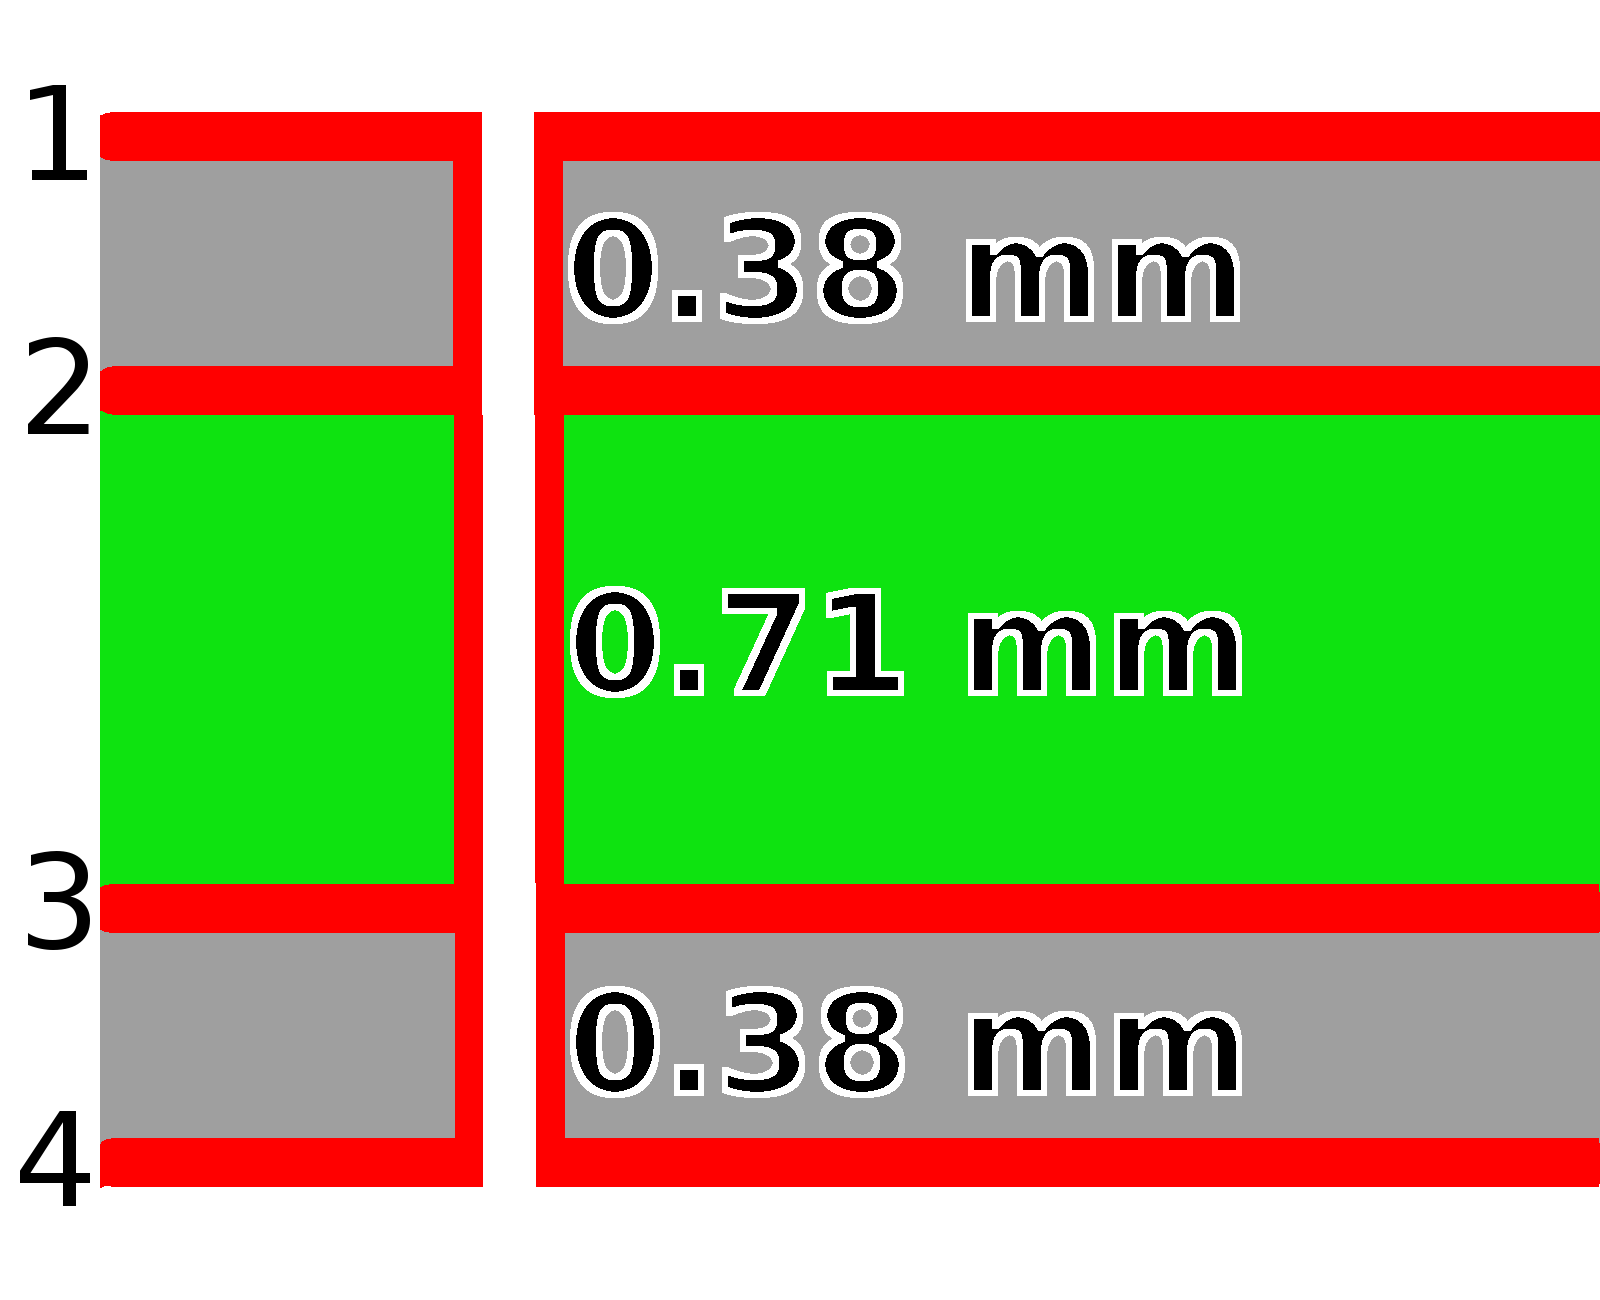
\includegraphics[width=0.3\textwidth]{TeilB/teilb_lagenaufbau.png}}
%			\fbox{	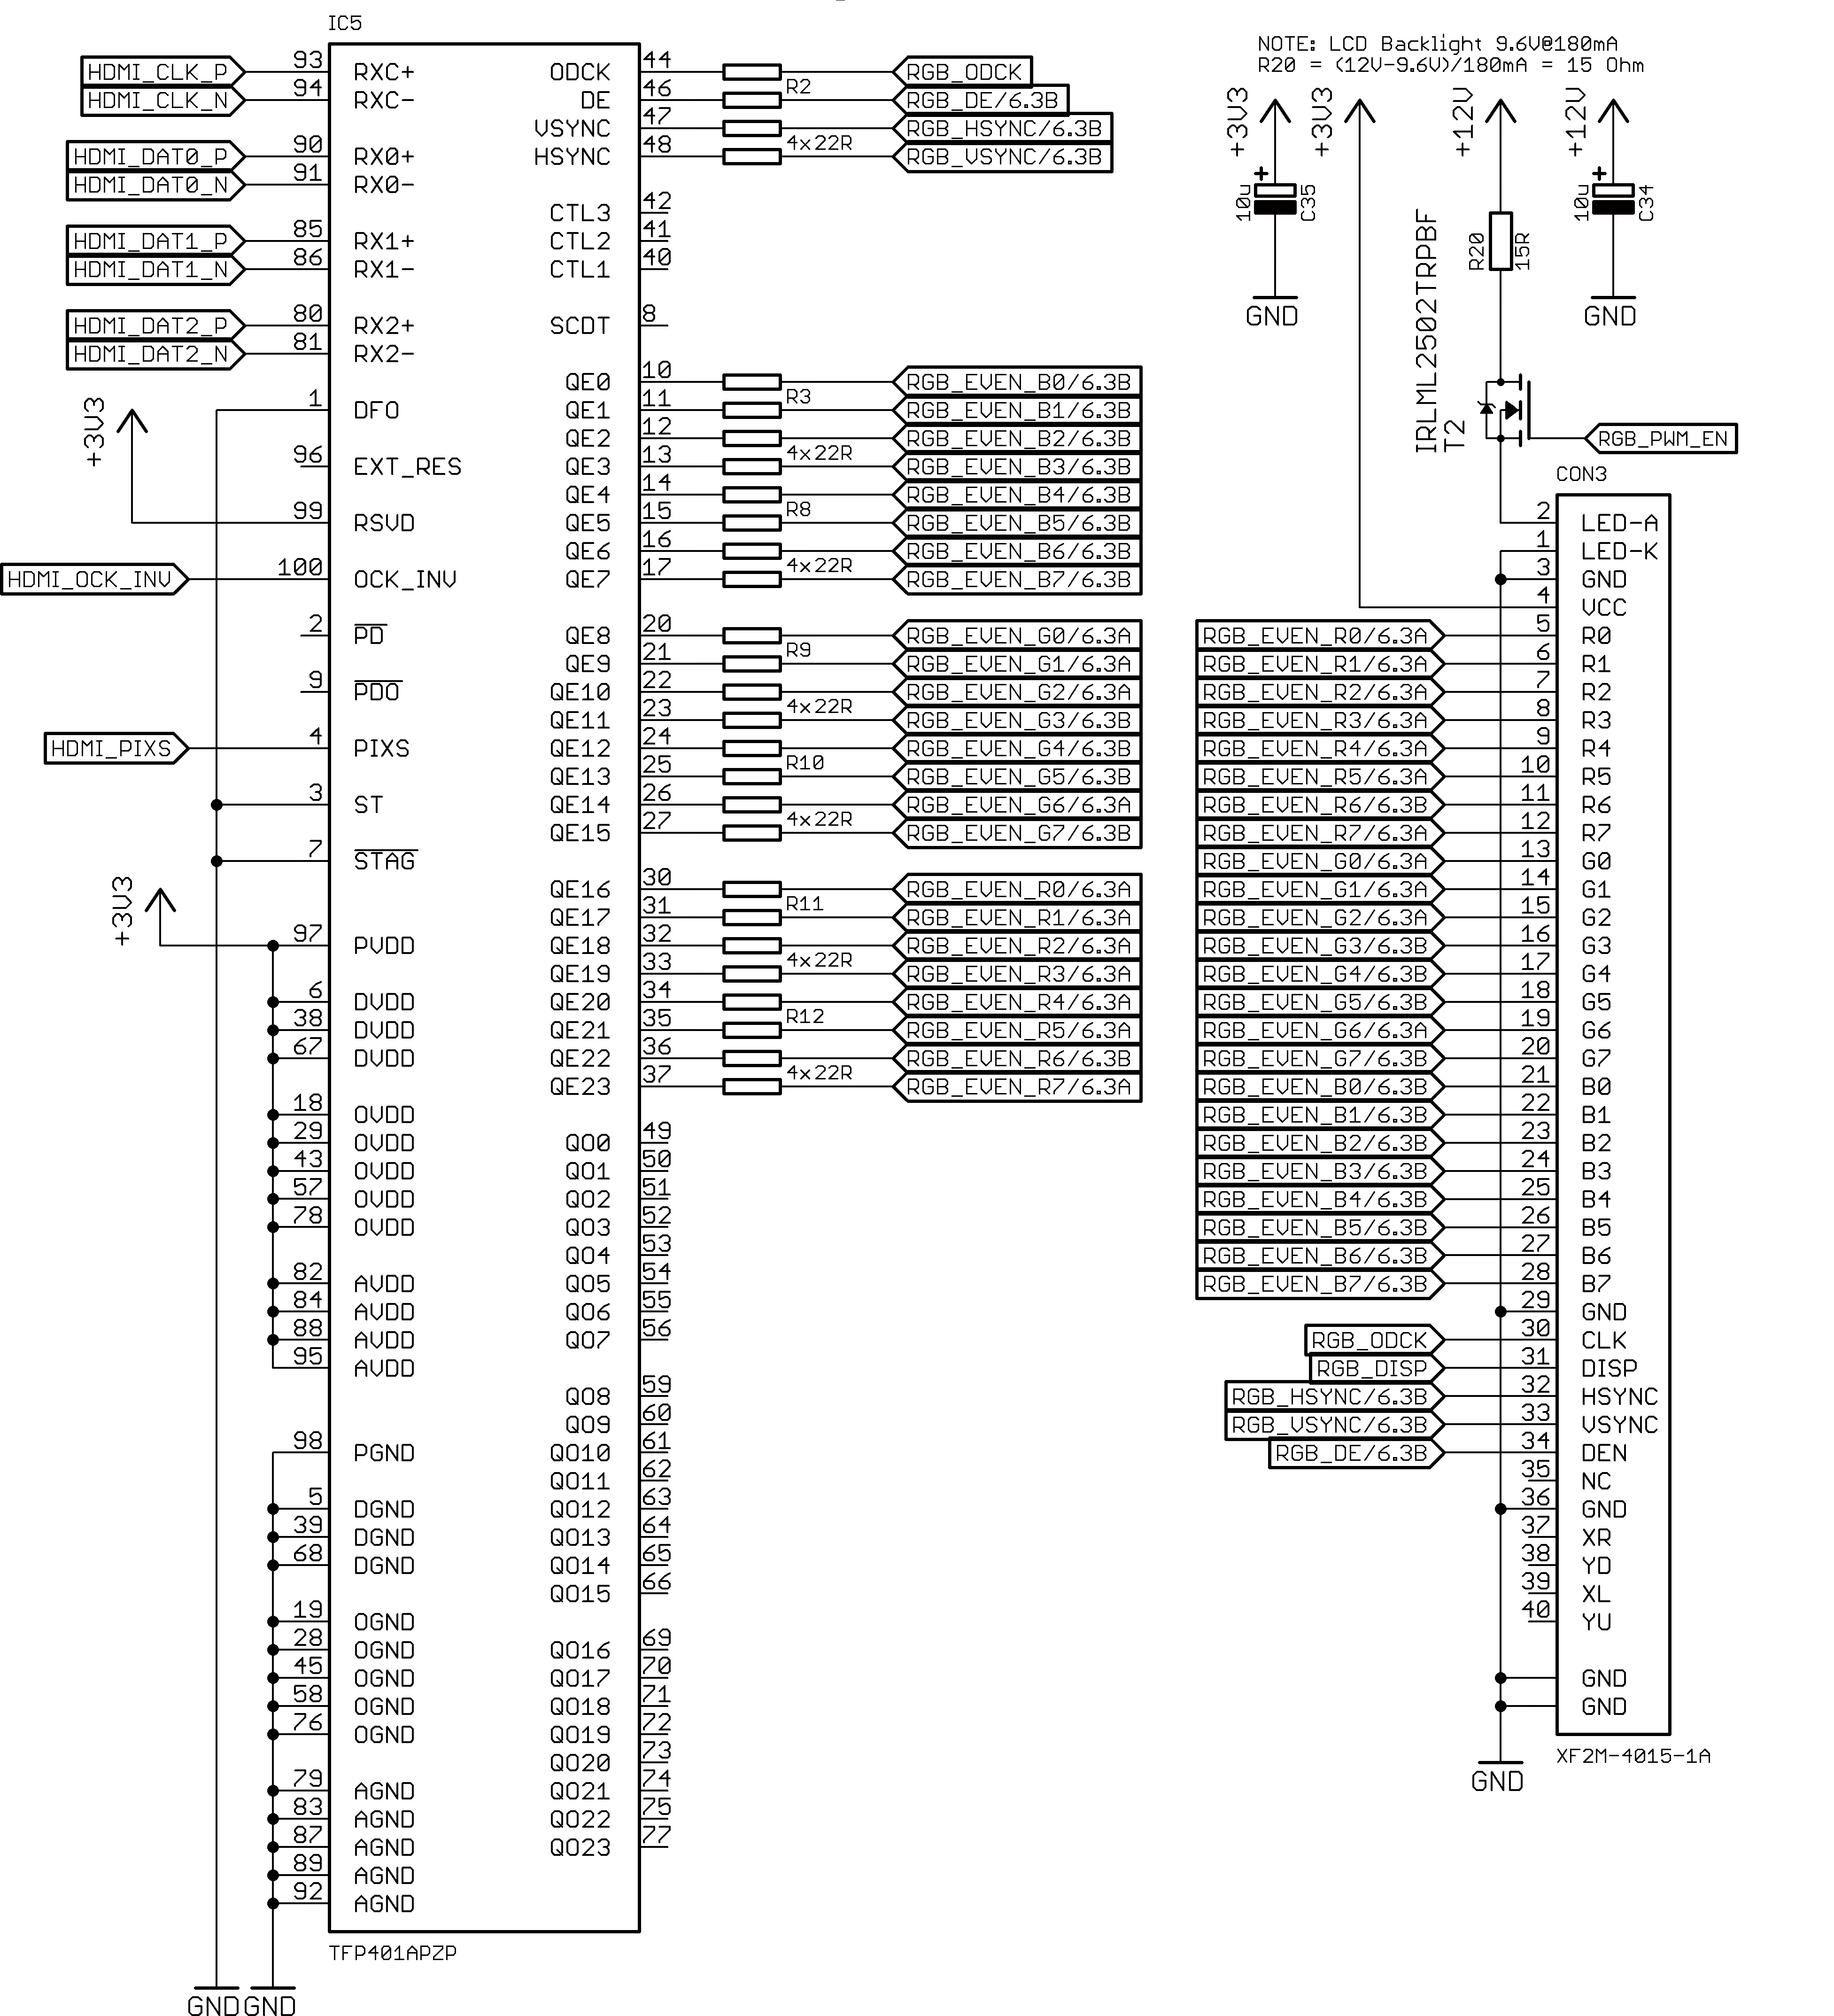
\includegraphics[width=8.5cm,keepaspectratio]{TeilB/rgb_bridge_sch.png}}
            \caption{Lagenaufbau Teil B}
            \label{fig:teilb_lagenaufbau}
        \end{figure}

\subsection{HDMI-Eingang}
\label{cha:hdmi_eingang}
Der HDMI-Eingang wird durch eine HDMI-Buchse der Firma \code{FCI} realisiert und wird mittels Impedanzkontrollierten Leitungen an die RGB-Bridge weitergegeben. Diese Leitungen sind mit einer differentielle Impedanz von 100\,$\Omega$ spezifiziert. Zu beachten ist, dass alle Leitungspaare dieselbe Länge aufweisen, da sonst Laufzeitunterschiede und Fehlabtastung innerhalb der verschiedenen Signalpaare auftreten und zu Fehlern führen können. Die Impedanz der differentieller Leitungen lässt sich nach den Gleichungen 
%
\begin{equation}
Z_0 = \frac{88.75}{\sqrt{\epsilon_r + 1.47}} \cdot ln\left(\frac{5.97 \cdot h}{0.8 \cdot W + t}\right)
\label{equ:z_0}
\end{equation}
%
und
%
\begin{equation}
Z_{Diff} = 2 \cdot Z_0  \cdot \left(1-0.48 \cdot e^{-0.96\frac{s}{h}}\right)
\label{equ:z_diff}
\end{equation}
%
mit den Parametern entsprechend \reft{tab:z_parameter} (siehe \cite{TI2007}) berechnen. Hier erhält man eine Impedanz $Z_0$ von 77\,$\Omega$ und eine differentielle Impedanz von 106\,$\Omega$. Aufgrund der kurzen Leitungslängen von maximal 11\,mm, spielt diese minimale Fehlanpassung keine große Rolle und kann vernachlässigt werden. Die Terminierung findet im Baustein statt und bedarf keiner externen Widerstände an den Enden der Leitungen.
\begin{table}[h]
\begin{tabular}{|p{7cm}|p{3cm}|p{3cm}|}\hline
\rowcolor{TableBackgroundColor} 
   \textbf{Parameter} & \textbf{Bezeichnung} & \textbf{Wert}	\\ \hline
    Dielektrikum 					& $\epsilon_r$	& 4.2		\\ \hline
	Breite der Leitungen  		 	& W 			& 0.28 mm	\\ \hline
	Abstand des Paares zueinander 	& s 			& 0.17 mm 	\\ \hline
	Dicke des Dielektrikums 		& h 			& 0.35 mm 	\\ \hline 
	Dicke der Leiterbahn 			& t 			& 35 µm		\\ \hline 
\end{tabular}
\caption{Parameter bezüglich Impedanz der HDMI-Leitungen}
\label{tab:z_parameter}
\end{table} \\
\refa{fig:teilb_hdmi} zeigt den Schaltplan und das Layout des HDMI-Steckeres. In \refa{fig:teilb_hdmi_pcb} sind die TMDS-Leitungspaare zu sehen, bei der ein gleichmäßiger Abstand zwischen den Leitungen einzelner Paare, sowie die gleiche Länge der Paare selbst eingehalten wird. 


\begin{figure}[htbp]
        %\begin{center}
        \centering
        \begin{subfigure}[htp]{0.48\textwidth}
%			\fbox{	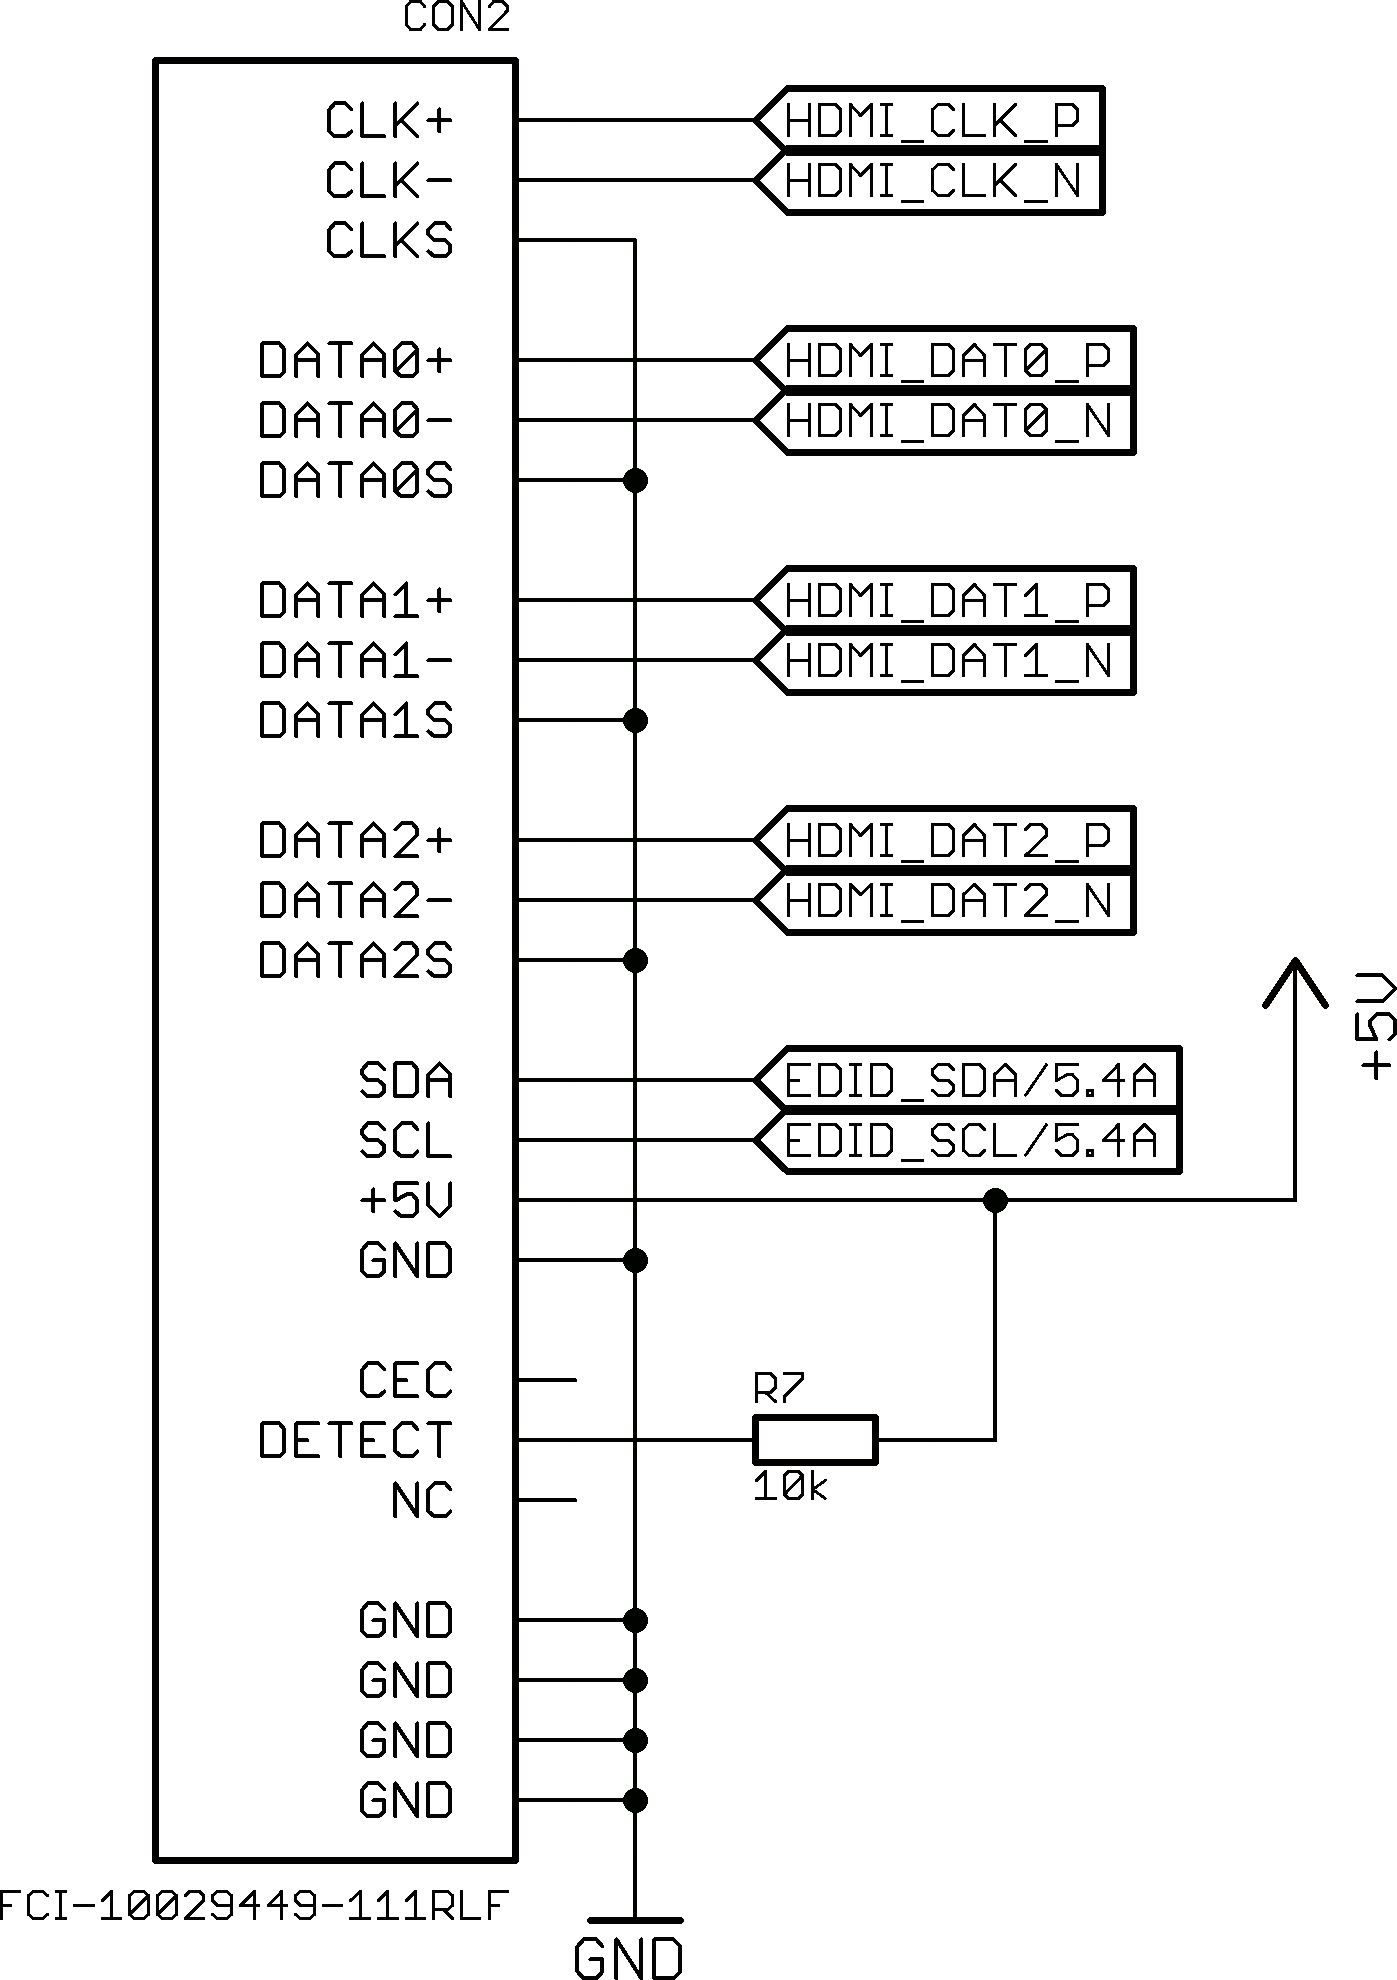
\includegraphics[width=1\textwidth]{TeilB/hdmi_sch.png}}
			\fbox{	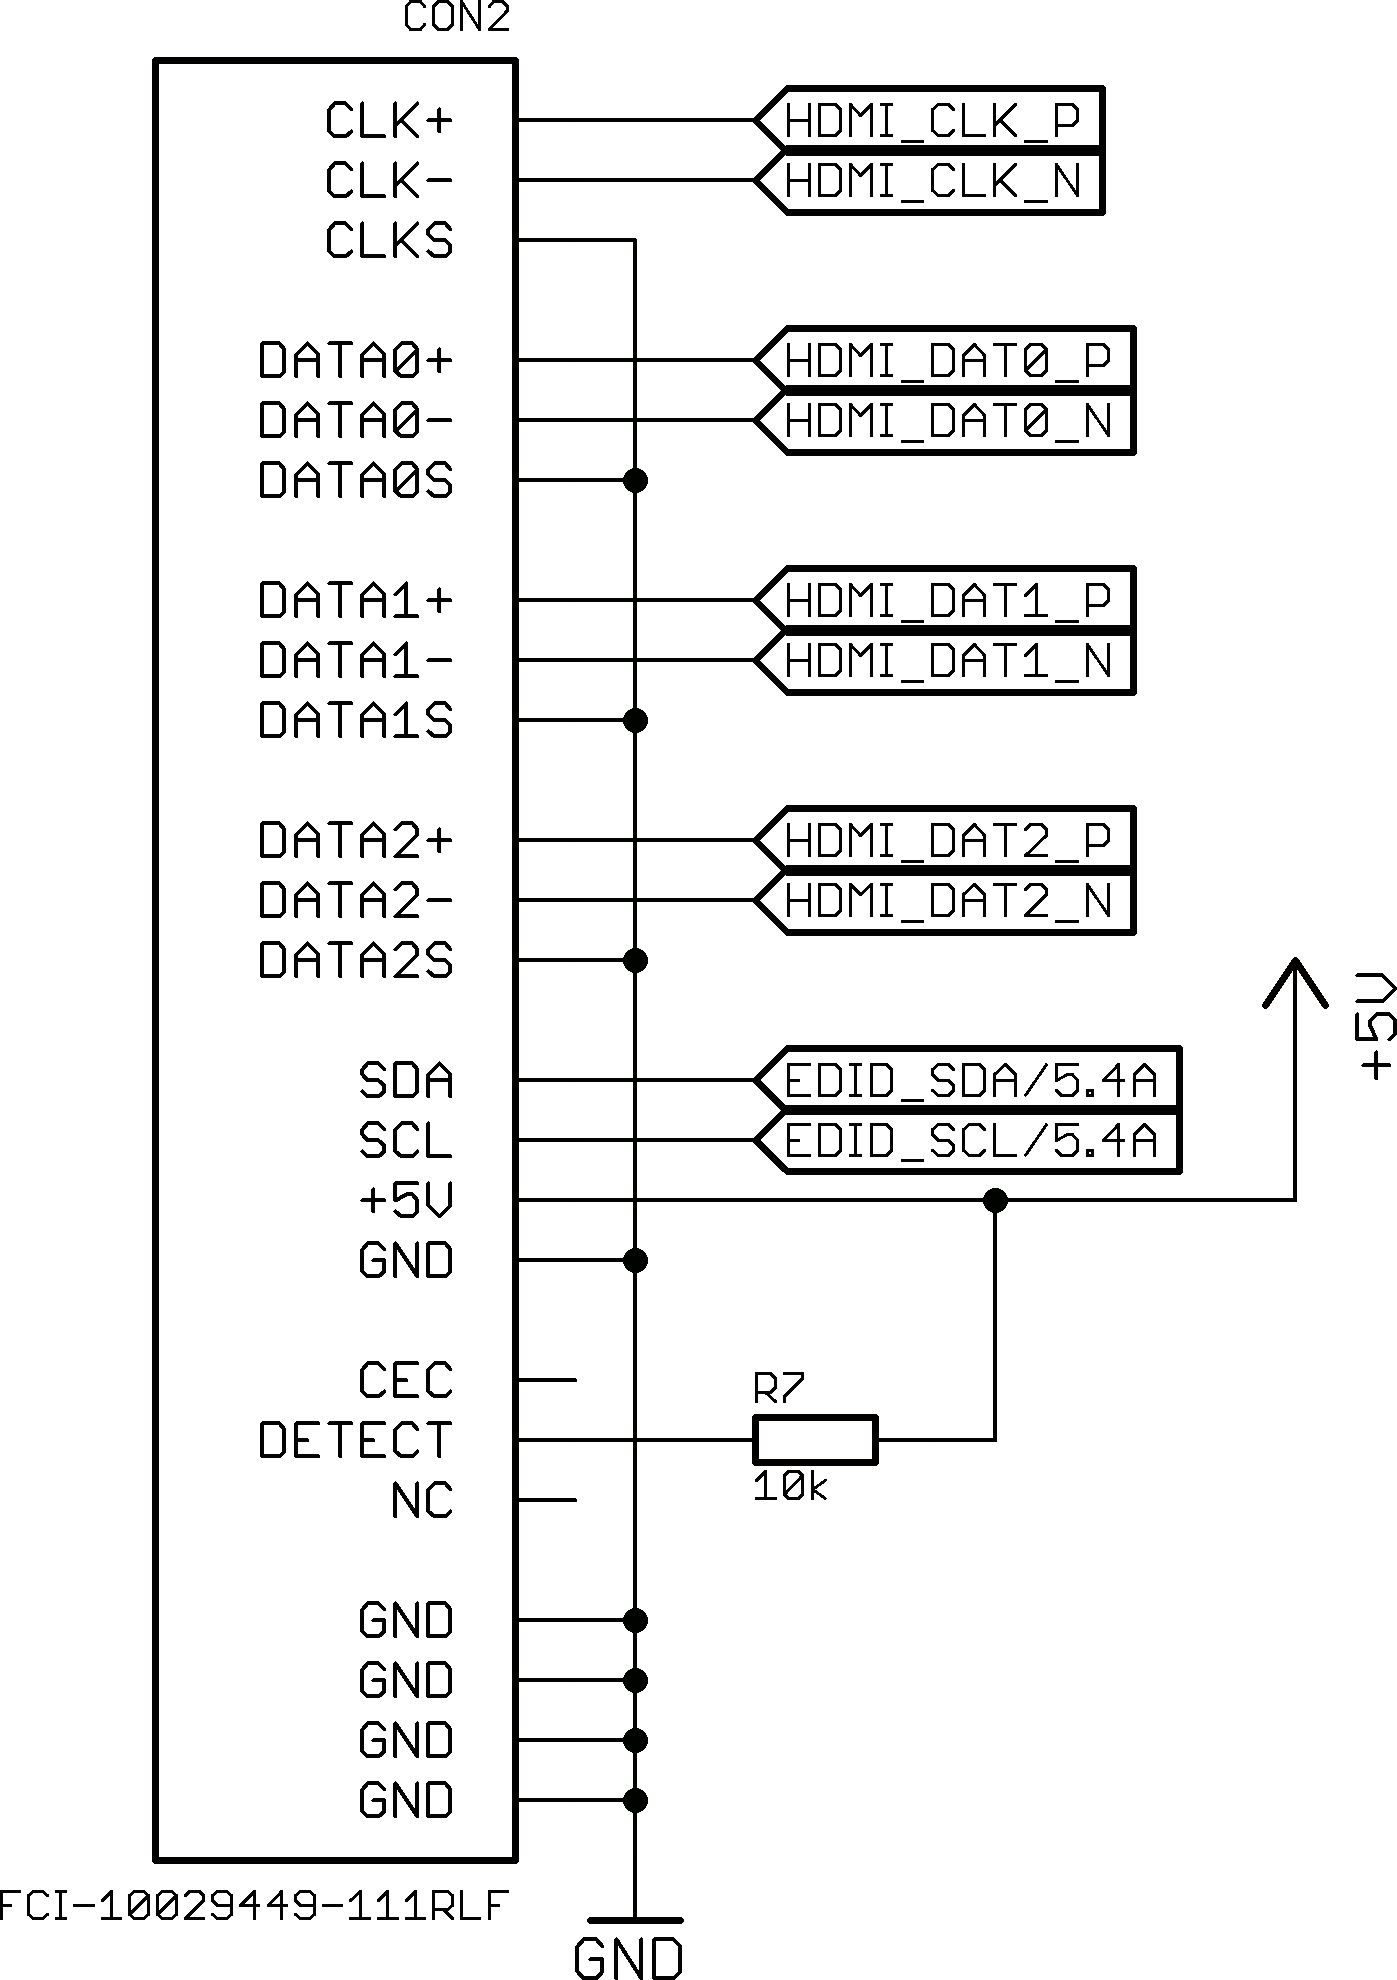
\includegraphics[height=6.5cm,width=1\textwidth,keepaspectratio]{TeilB/hdmi_sch.png}}
            \caption{HDMI-Stecker: Schaltplan}
            \label{fig:teilb_hdmi_sch}
        \end{subfigure}
\quad 
        \begin{subfigure}[htp]{0.48\textwidth}
			\fbox{	\includegraphics[height=6.5cm,width=1\textwidth,keepaspectratio]{TeilB/hdmi_stecker.png}}
 			\caption{HDMI Stecker: Layout}
            \label{fig:teilb_hdmi_pcb}
        \end{subfigure}
		%\end{center}
        \caption{HDMI Leitungen}
        \label{fig:teilb_hdmi}
\end{figure}
Neben den eigentlichen Video-Signalen befinden sich noch die $I^2C$-Signale \code{EDID_SCL}\footnote{EDID\_SCL: Taktleitung des $I^2C$-Bus} und \code{EDID_SDA}\footnote{EDID\_SDA: Datenleitung des $I^2C$-Bus} des EDID-EEPROMs sowie eine Hot-Plug-Detection auf der HDMI-Buchse.
\subsection{RGB-Bridge}
Die Eingänge der RGB-Bridge werden vom HDMI-Stecker gespeist. Die TMDS-Signale werden so aufbereitet, dass an den Ausgängen eine RGB-Schnittstelle zum Anschluss eines RGB-Panels bereitgestellt sind.
        \begin{figure}[htp]
        	\center
			\fbox{	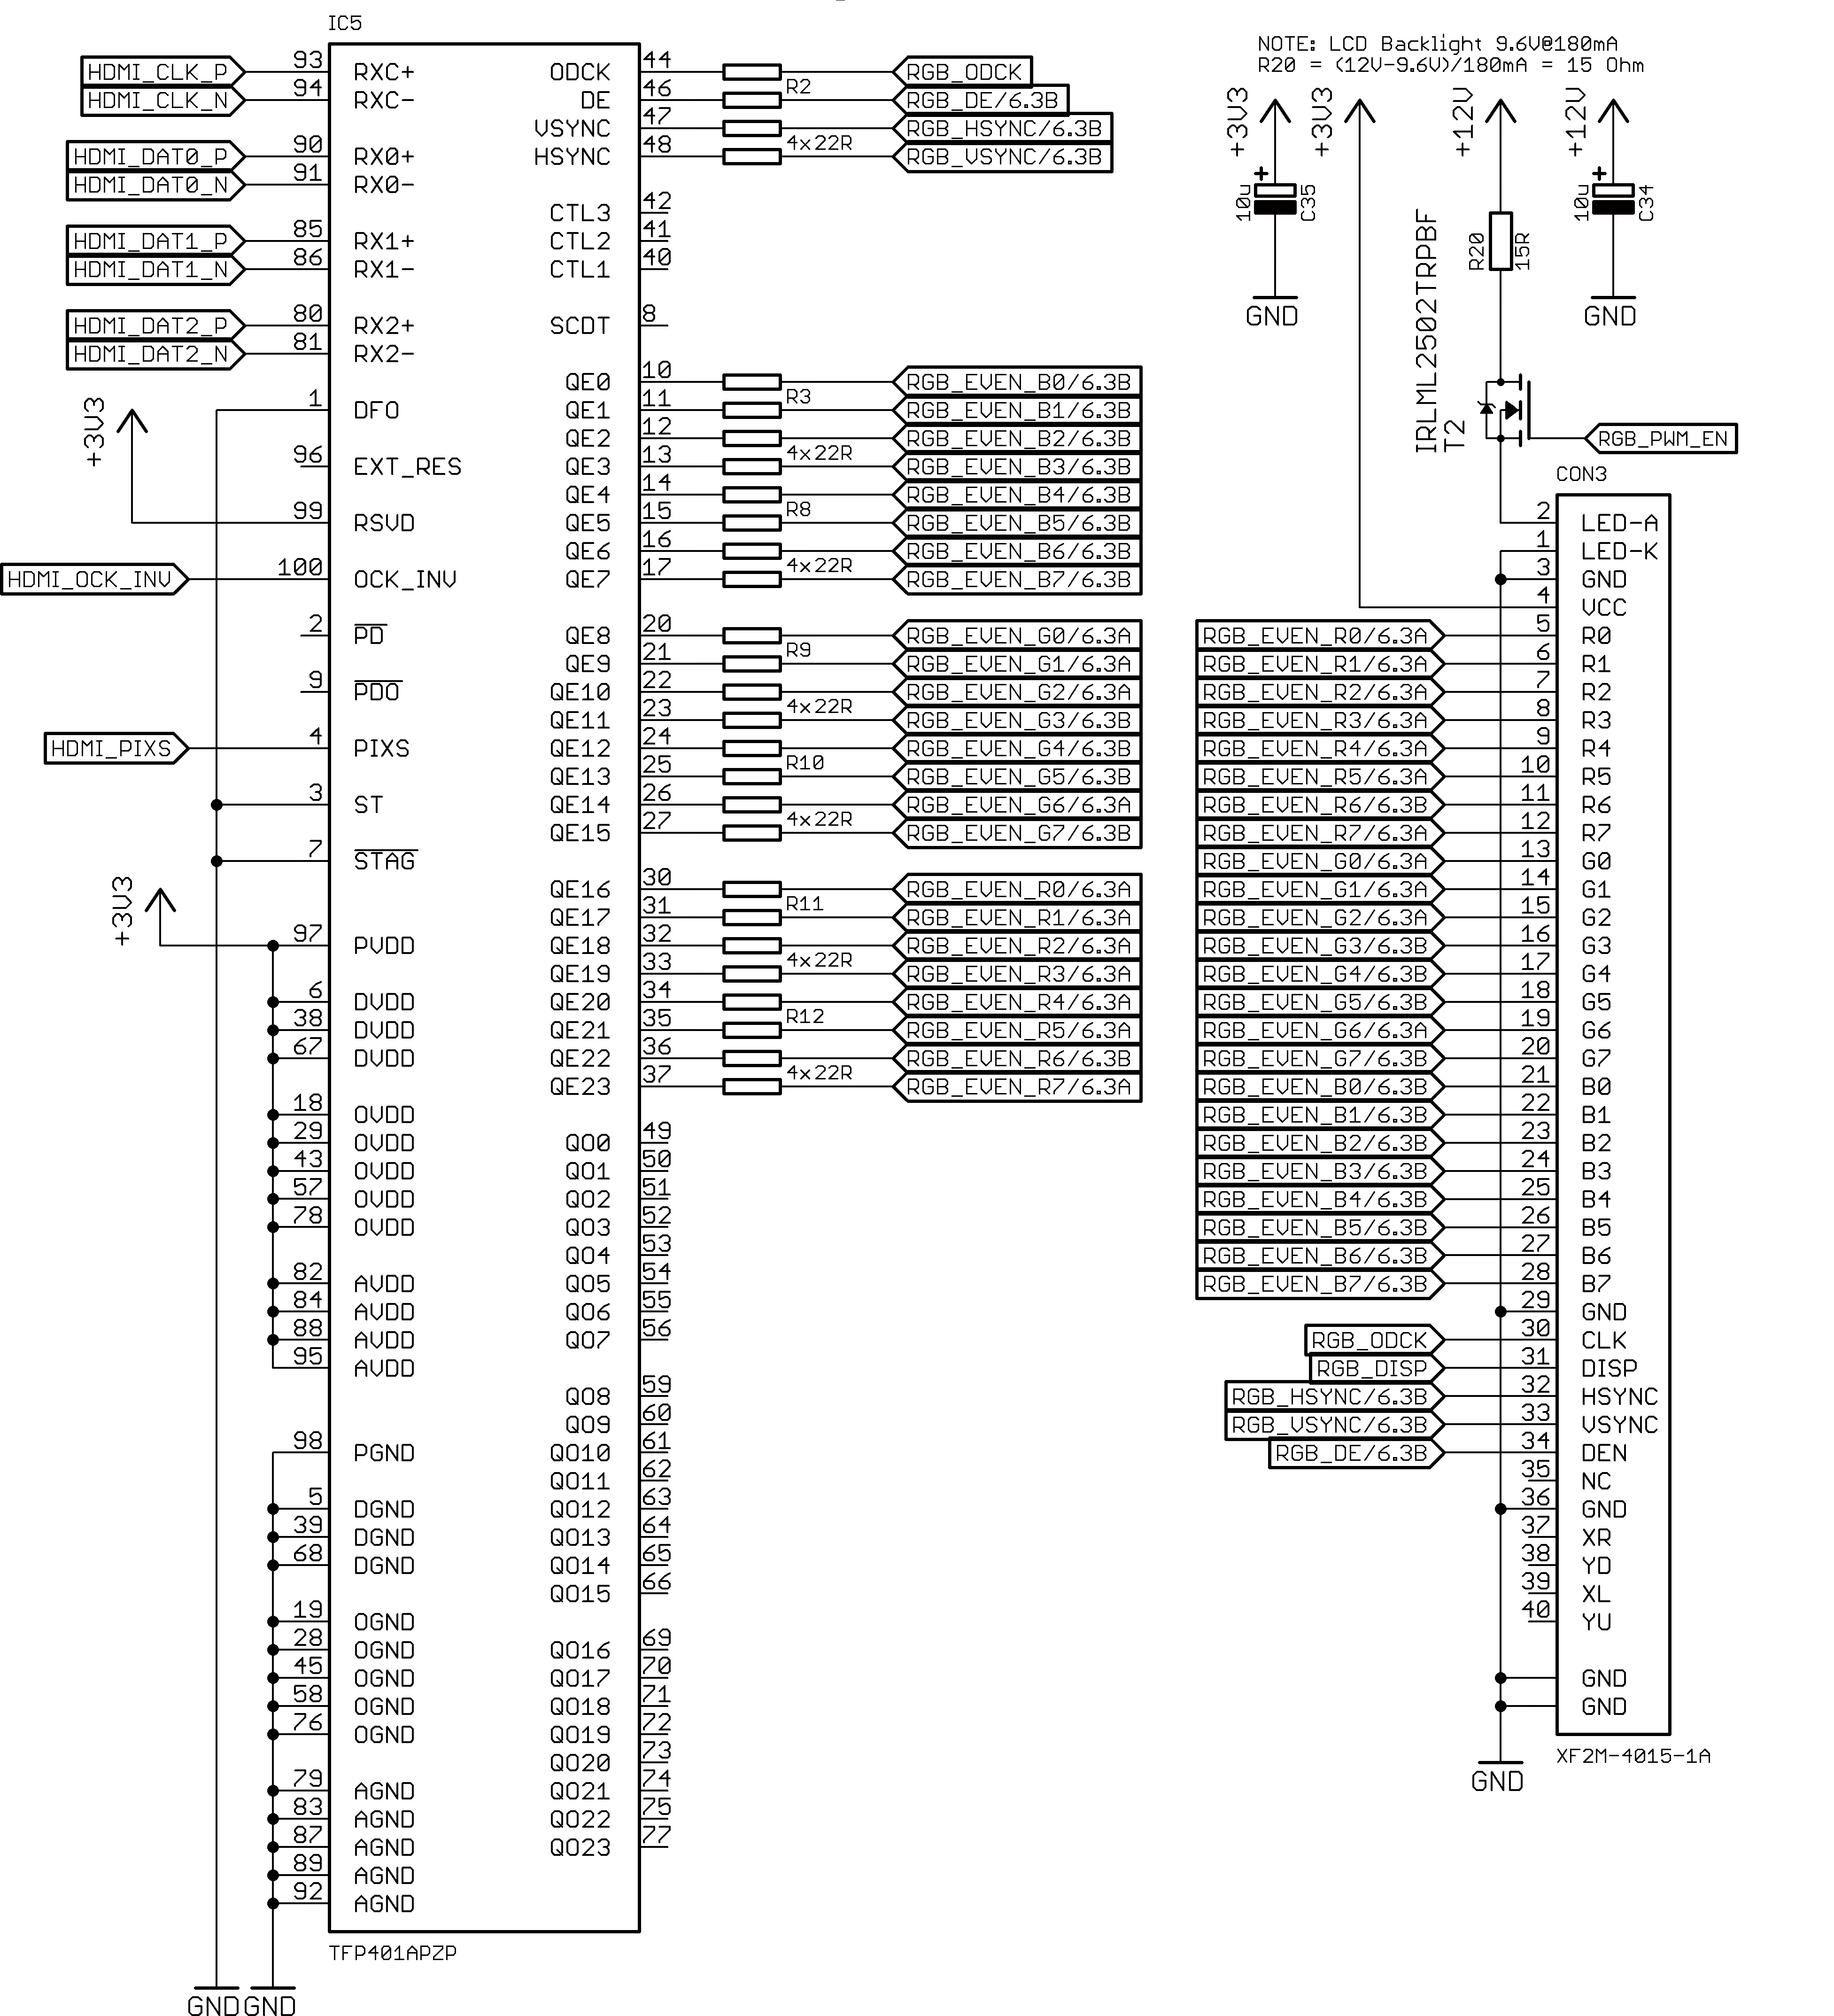
\includegraphics[width=0.9\textwidth]{TeilB/rgb_bridge_sch.png}}
%			\fbox{	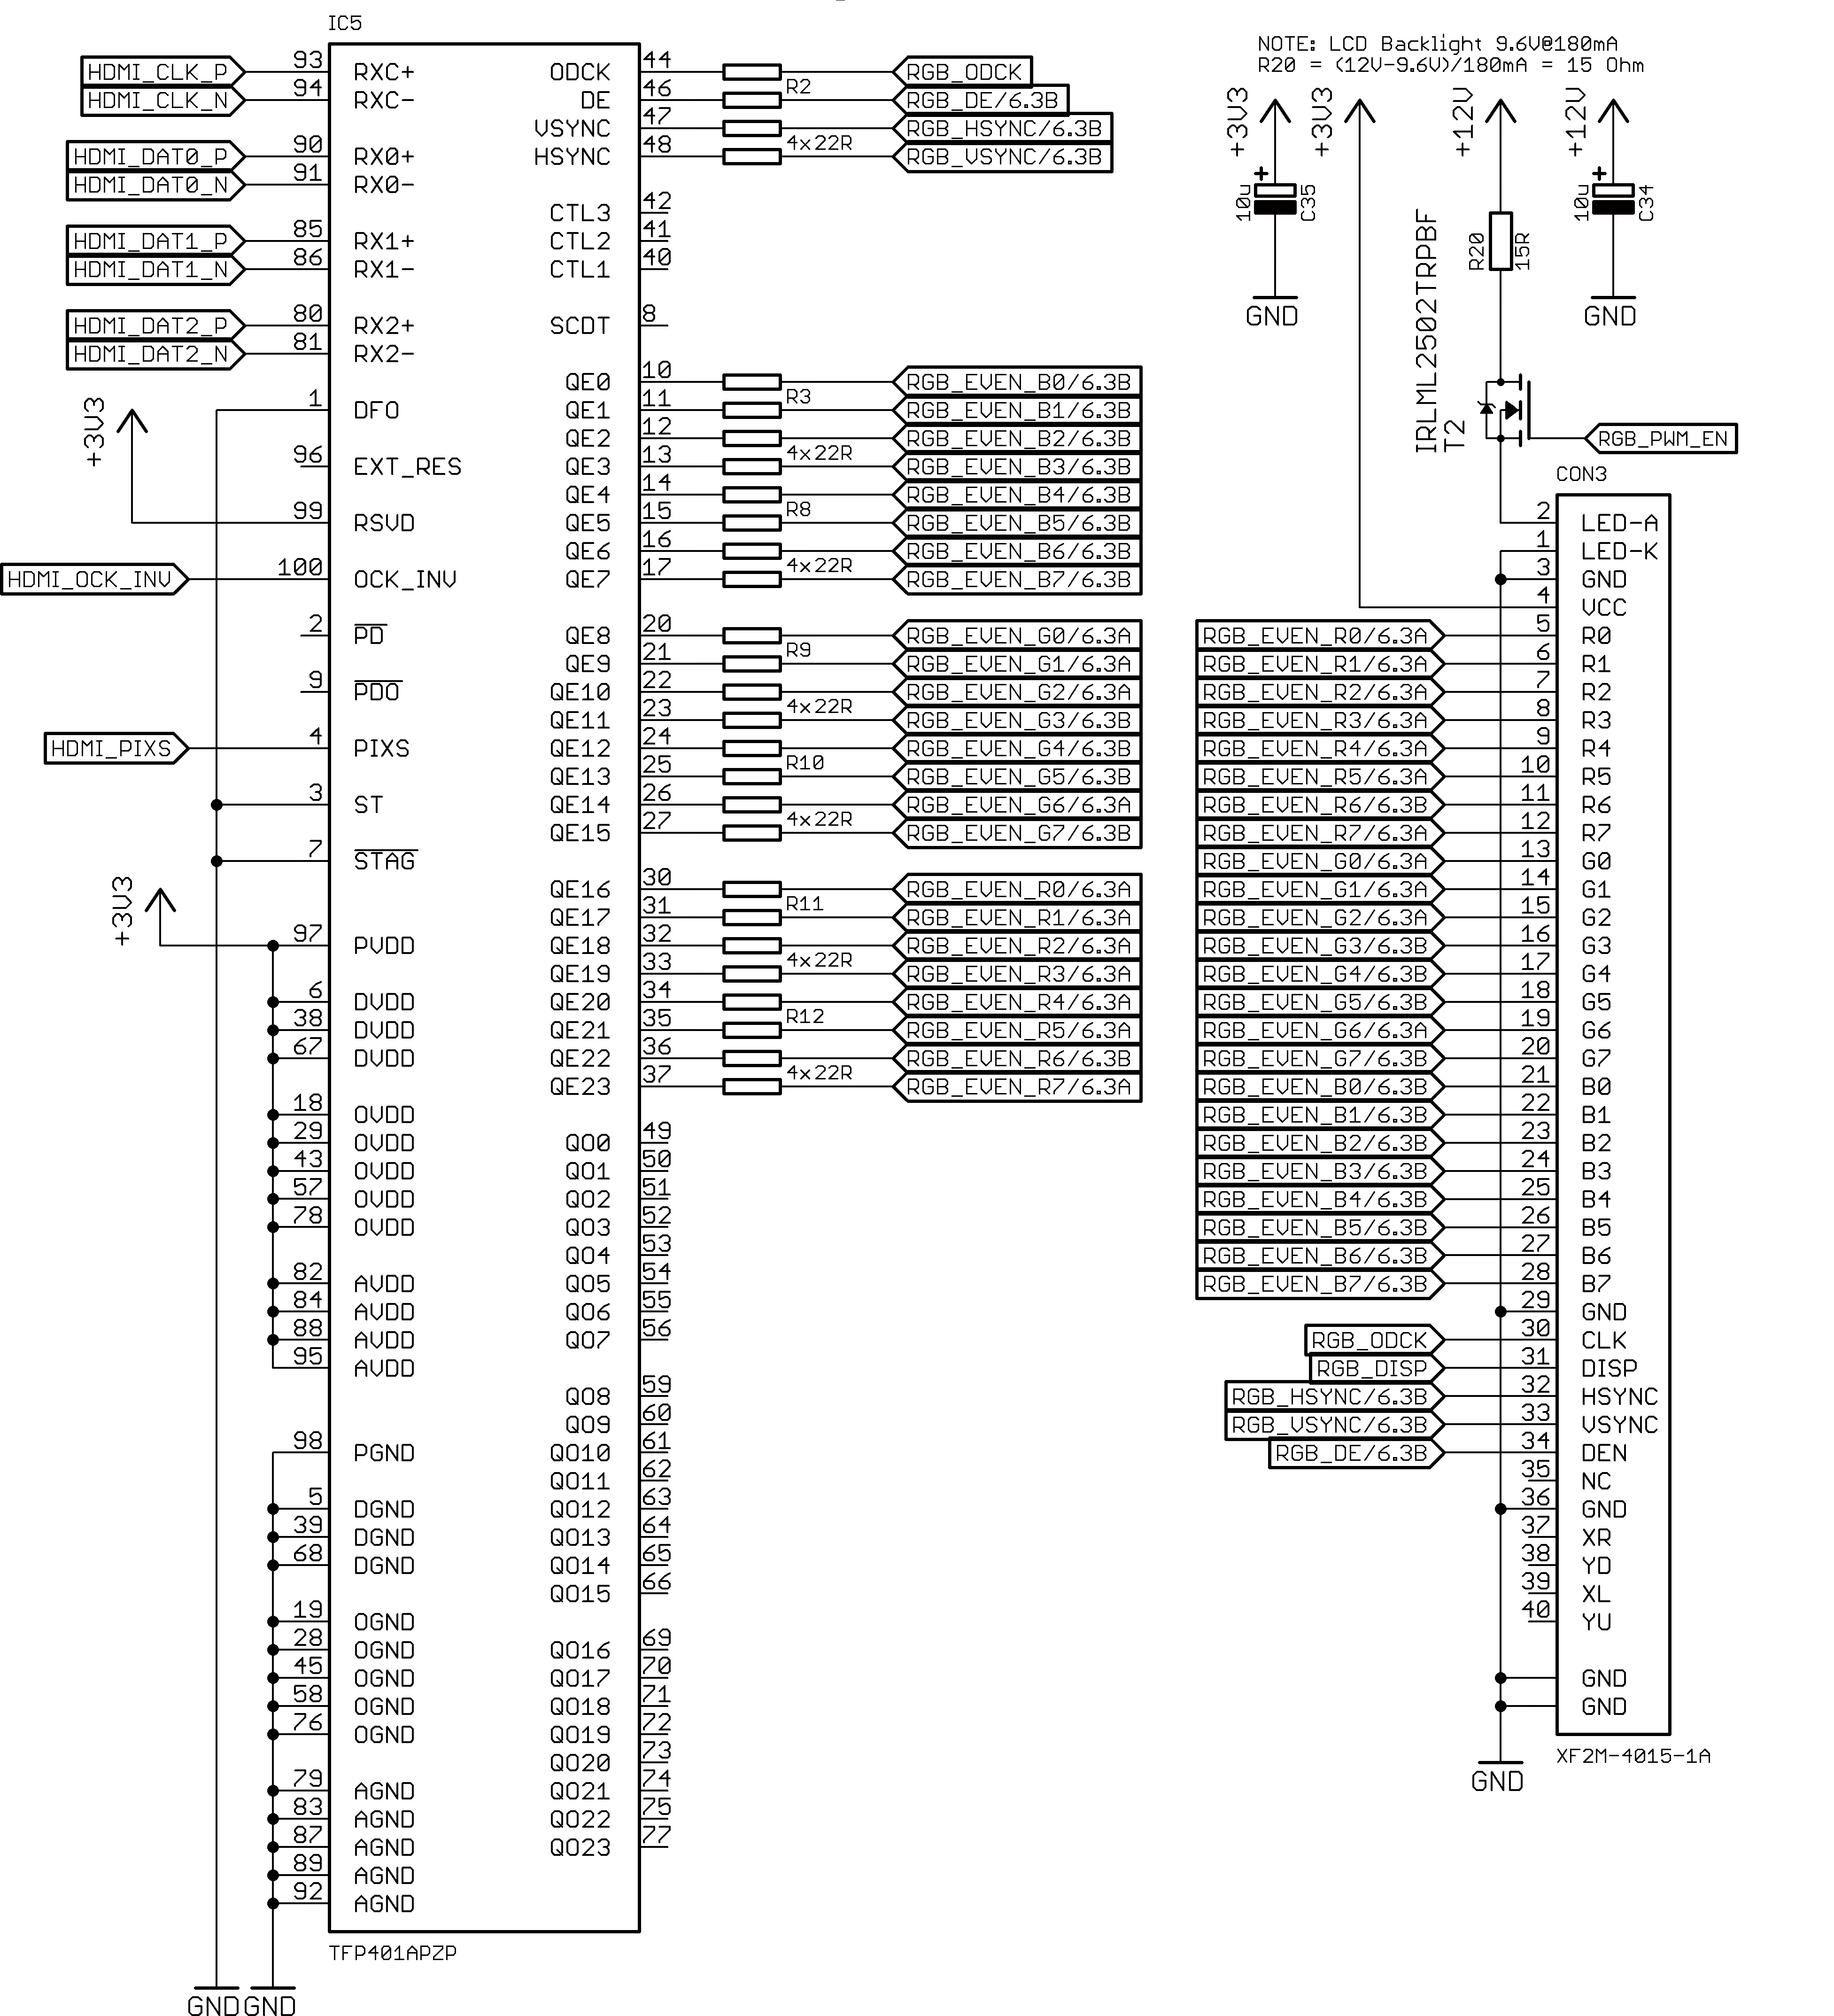
\includegraphics[width=8.5cm,keepaspectratio]{TeilB/rgb_bridge_sch.png}}
            \caption{RGB Bridge: Schaltplan}
            \label{fig:teilb_rgb_bridge_sch}
        \end{figure}
\newline        
\refa{fig:teilb_rgb_bridge_sch} zeigt den Schaltplan der RGB-Bridge mit dem Stecker für das RGB-Display. Als Baustein ist ein \code{TFP401A} von Texas Instruments im Einsatz. Neben den vier TMDS-Signalpaaren werden eingangsseitig noch die Signale \code{HDMI_PIXS} und \code{HDMI_OCK_INV} eingespeist. Diese sind zur Konfiguration der Ausgangssignale vorhanden. Ausgangsseitig sind die drei Farbkanäle für Rot, Grün und Blau (\code{RGB_EVEN_R[7:0]}, \code{RGB_EVEN_G[7:0]} und \code{RGB_EVEN_B[7:0]}) sowie die Steuersignale \code{RGB_ODCK}, \code{RGB_DE}, \code{RGB_HSYNC} und \code{RGB_VSYNC} verbunden.
Fließen Ströme mit hoher Frequenz, entstehen aufgrund des Induktionsgesetzes Störeffekte auf den Leitungen, die wiederum andere Signale beeinflussen können. Die induzierte Störspannung lässt sich mit der Gleichung
%
\begin{equation}
u \approx L \cdot \frac{di}{dt}
\label{equ:induzierte_spannung}
\end{equation}
%
berechnen. Steigt die Schaltfrequenz, und damit die Frequenz der Stromänderung $\frac{di}{dt}$, wird die abgestrahlte Störung ebenfalls stärker. Um diesem Effekt entgegenzuwirken, sind Serienwiderstände im Signalweg eingebaut, die mit der natürlichen Kapazität der Leitung den Tiefpasscharakter der Leitung besser ausprägt. Die Kapazität einer Mikrostreifenleitung lässt sich mit 
%
\begin{equation}
C_{Leiterbahn} = \epsilon_0 \cdot \epsilon_r \cdot \frac{(a+b) \cdot l}{d}
\label{equ:c_leiterbahn}
\end{equation}
%
für $\epsilon_0 = 8.86\cdot10^{-12} \frac{Am}{Vs}$, $\epsilon_r = 4.2$, der Leiterbahnbreite $a = 0.15 $mm, der Leiterbahndicke $b = 35$ µm, dem Abstand zur nächsten Fläche $d = 0.35$ mm und der durchschnittlichen Leiterbahnlänge $l = 50$ mm berechnen (siehe \cite{Gensicke2014}). Die durchschnittliche Kapazität der RGB-Leitungen beträgt somit rund 1\,pF. In Verbindung mit dem verwendeten 22\,$\Omega$ Widerstand bildet dieser in Verbindung mit der Leitung einen Tiefpass. Der quantitative Verlauf des Tiefpass deutet sich in \refa{fig:teilb_tiefpass_mess} an, wobei Grün die originale und Blau die gefilterte Kurve darstellt. Zu erkennen ist, dass die Steilheit der fallenden und steigenden Flanke abnimmt, was zu einer verlangsamten Stromänderung $\frac{di}{dt}$ führt.
\begin{figure}[htbp]
			\fbox{	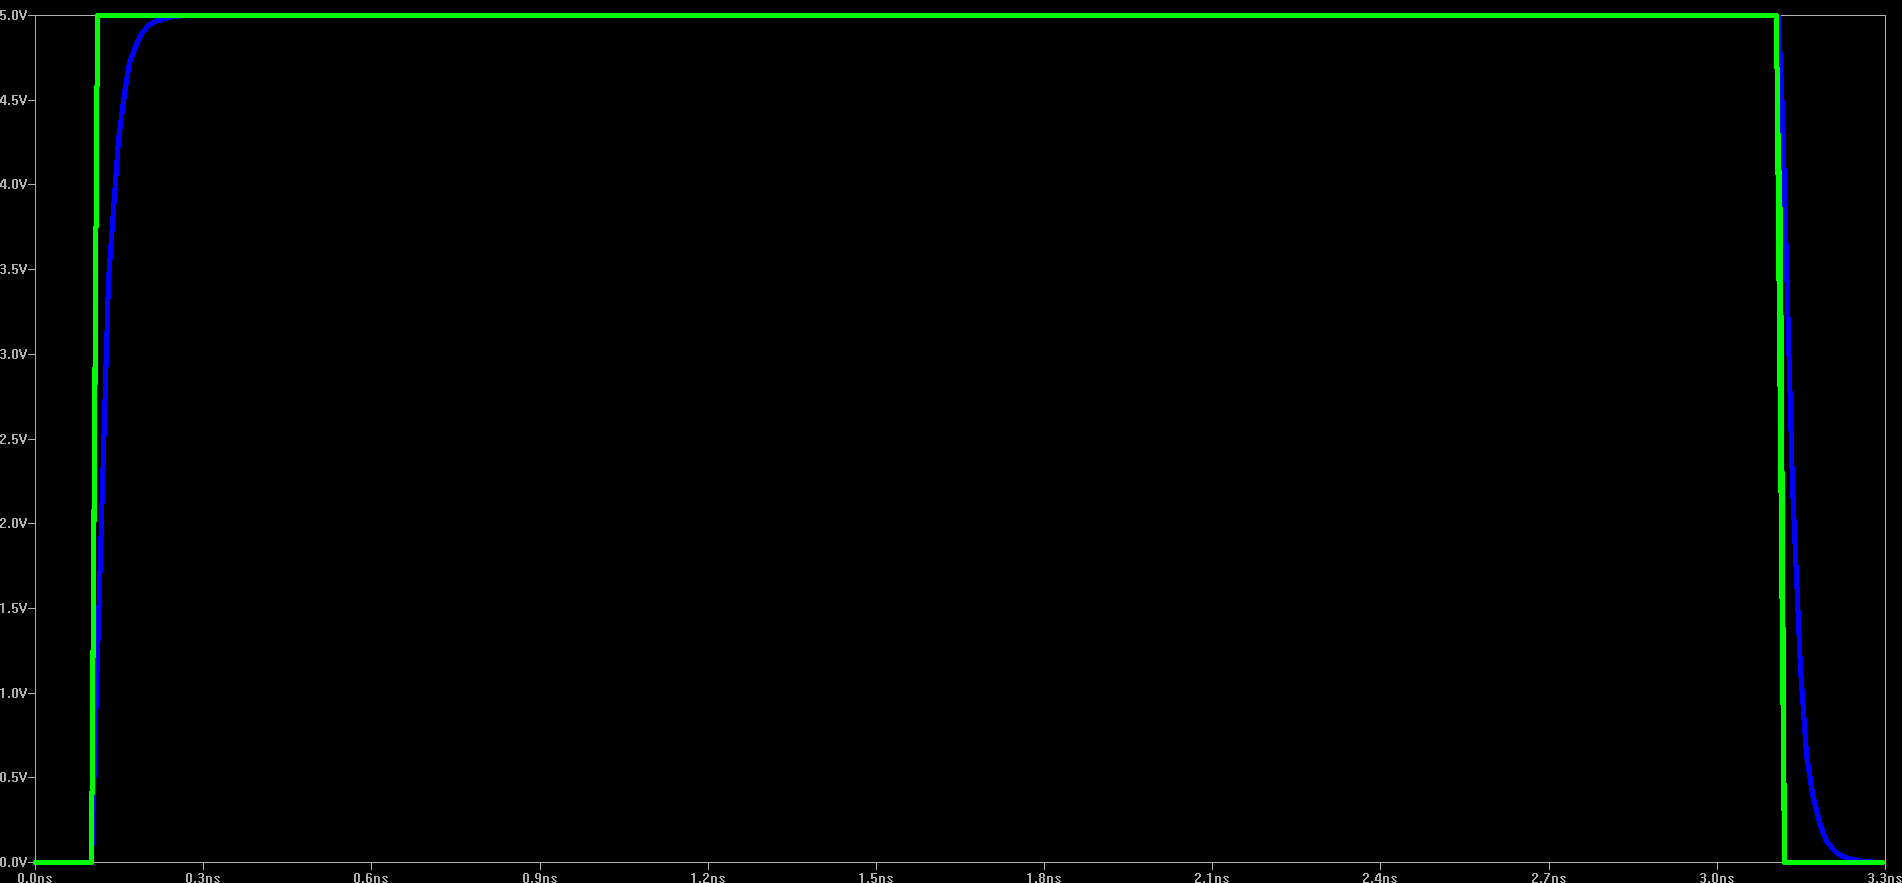
\includegraphics[width=1\textwidth,keepaspectratio]{TeilB/sim_serienwiderstand_messung.png}}
 			\caption{RGB Bridge: Simulationsergebnis des Leitungstiefpass}
            \label{fig:teilb_tiefpass_mess}
\end{figure}
Das Layout der RGB-Signale, gezeigt in \refa{fig:teilb_rgb_bridge_pcb}, ist unkritischer als das der HDMI-Signale, da beim verwendeten Display ein maximaler Pixeltakt von 33\,MHz auftritt (siehe \cite{LG2012}, S.14). Aufgrund der noch relativ langsamen Taktung, haben eventuell auftretende Laufzeitunterschiede zwischen den Signale einen vernachlässigbaren Effekt. Die Serienwiderstände sind als Widerstands-Array mit je vier realisiert.
\begin{figure}[htp]
	\center
	\fbox{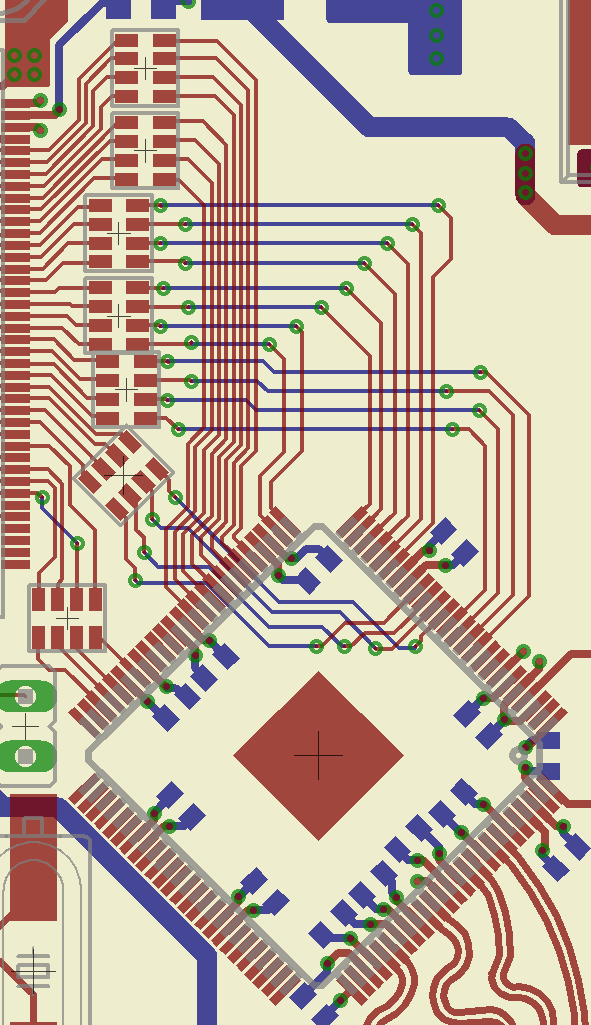
\includegraphics[height=0.8\textwidth,keepaspectratio,angle=90]{TeilB/rgb_bridge_pcb.png}}
 	\caption{RGB Bridge: Layout, gedreht um 90$^{\circ}$} 
    \label{fig:teilb_rgb_bridge_pcb}
\end{figure}
\newpage
\subsection{LVDS-Bridge}
Die LVDS-Bridge teilt die am Eingang liegenden parallelen RGB-Signale in Pakete zu je acht Bit auf und übertragt diese seriell über die verfügbaren LVDS-Kanäle. Die Beschaltung der LVDS-Bridge ist daher auf das verwendete Display \code{LB070WV8-SL01} zugeschnitten und analog den Abbildungen \ref{fig:teilb_lvds_bridge_format} und \ref{fig:teilb_lvds_display_format} zu verbinden.
\begin{figure}[htbp]
        %\begin{center}
        \begin{center}
        \begin{subfigure}[htp]{0.48\textwidth}
			\fbox{	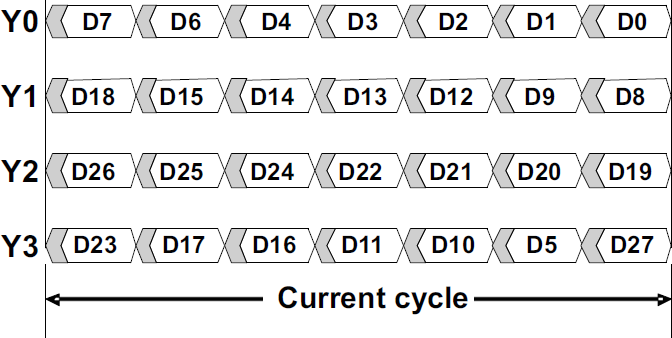
\includegraphics[height=3.3cm]{TeilB/lvds_bridge_paket.png}}
 			\caption{Paketformat LVDS-Bridge, \cite{TI2011b}}
            \label{fig:teilb_lvds_bridge_format}
        \end{subfigure}
        \quad
        \begin{subfigure}[htp]{0.48\textwidth}
			\fbox{	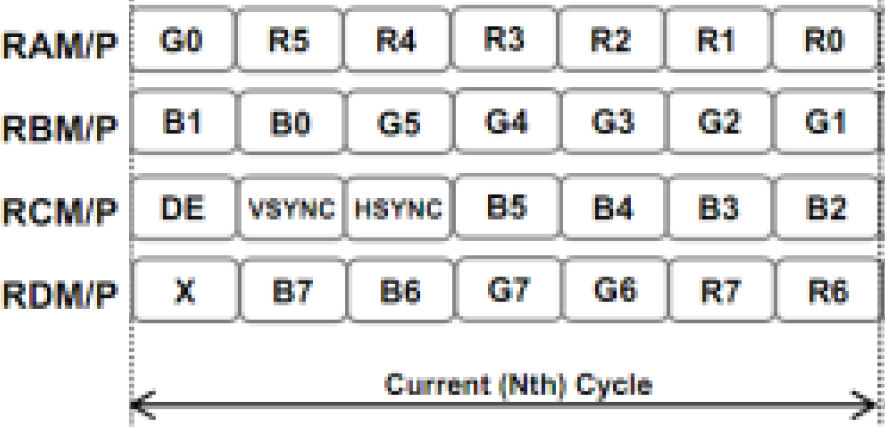
\includegraphics[height=3.3cm]{TeilB/lvds_display_paket.png}}
            \caption{Paketformat LVDS-Display, \cite{LG2012}}
            \label{fig:teilb_lvds_display_format}
        \end{subfigure}
		\end{center}
        \caption{LVDS Paketformate}
        \label{fig:teilb_lvds_format}
\end{figure} \\
So liegt zum Beispiel das RGB Bit G4 auf dem Dateneingang D13 der LVDS-Bridge. Der Schaltplan in \refa{fig:teilb_lvds_bridge_sch} zeigt die Beschaltung der LVDS-Bridge und des Steckverbinders für das Display.\\
\begin{figure}[htp]
		\center
		\fbox{	\includegraphics[width=0.8\textwidth]{TeilB/lvds_bridge_sch.png}}
%			\fbox{	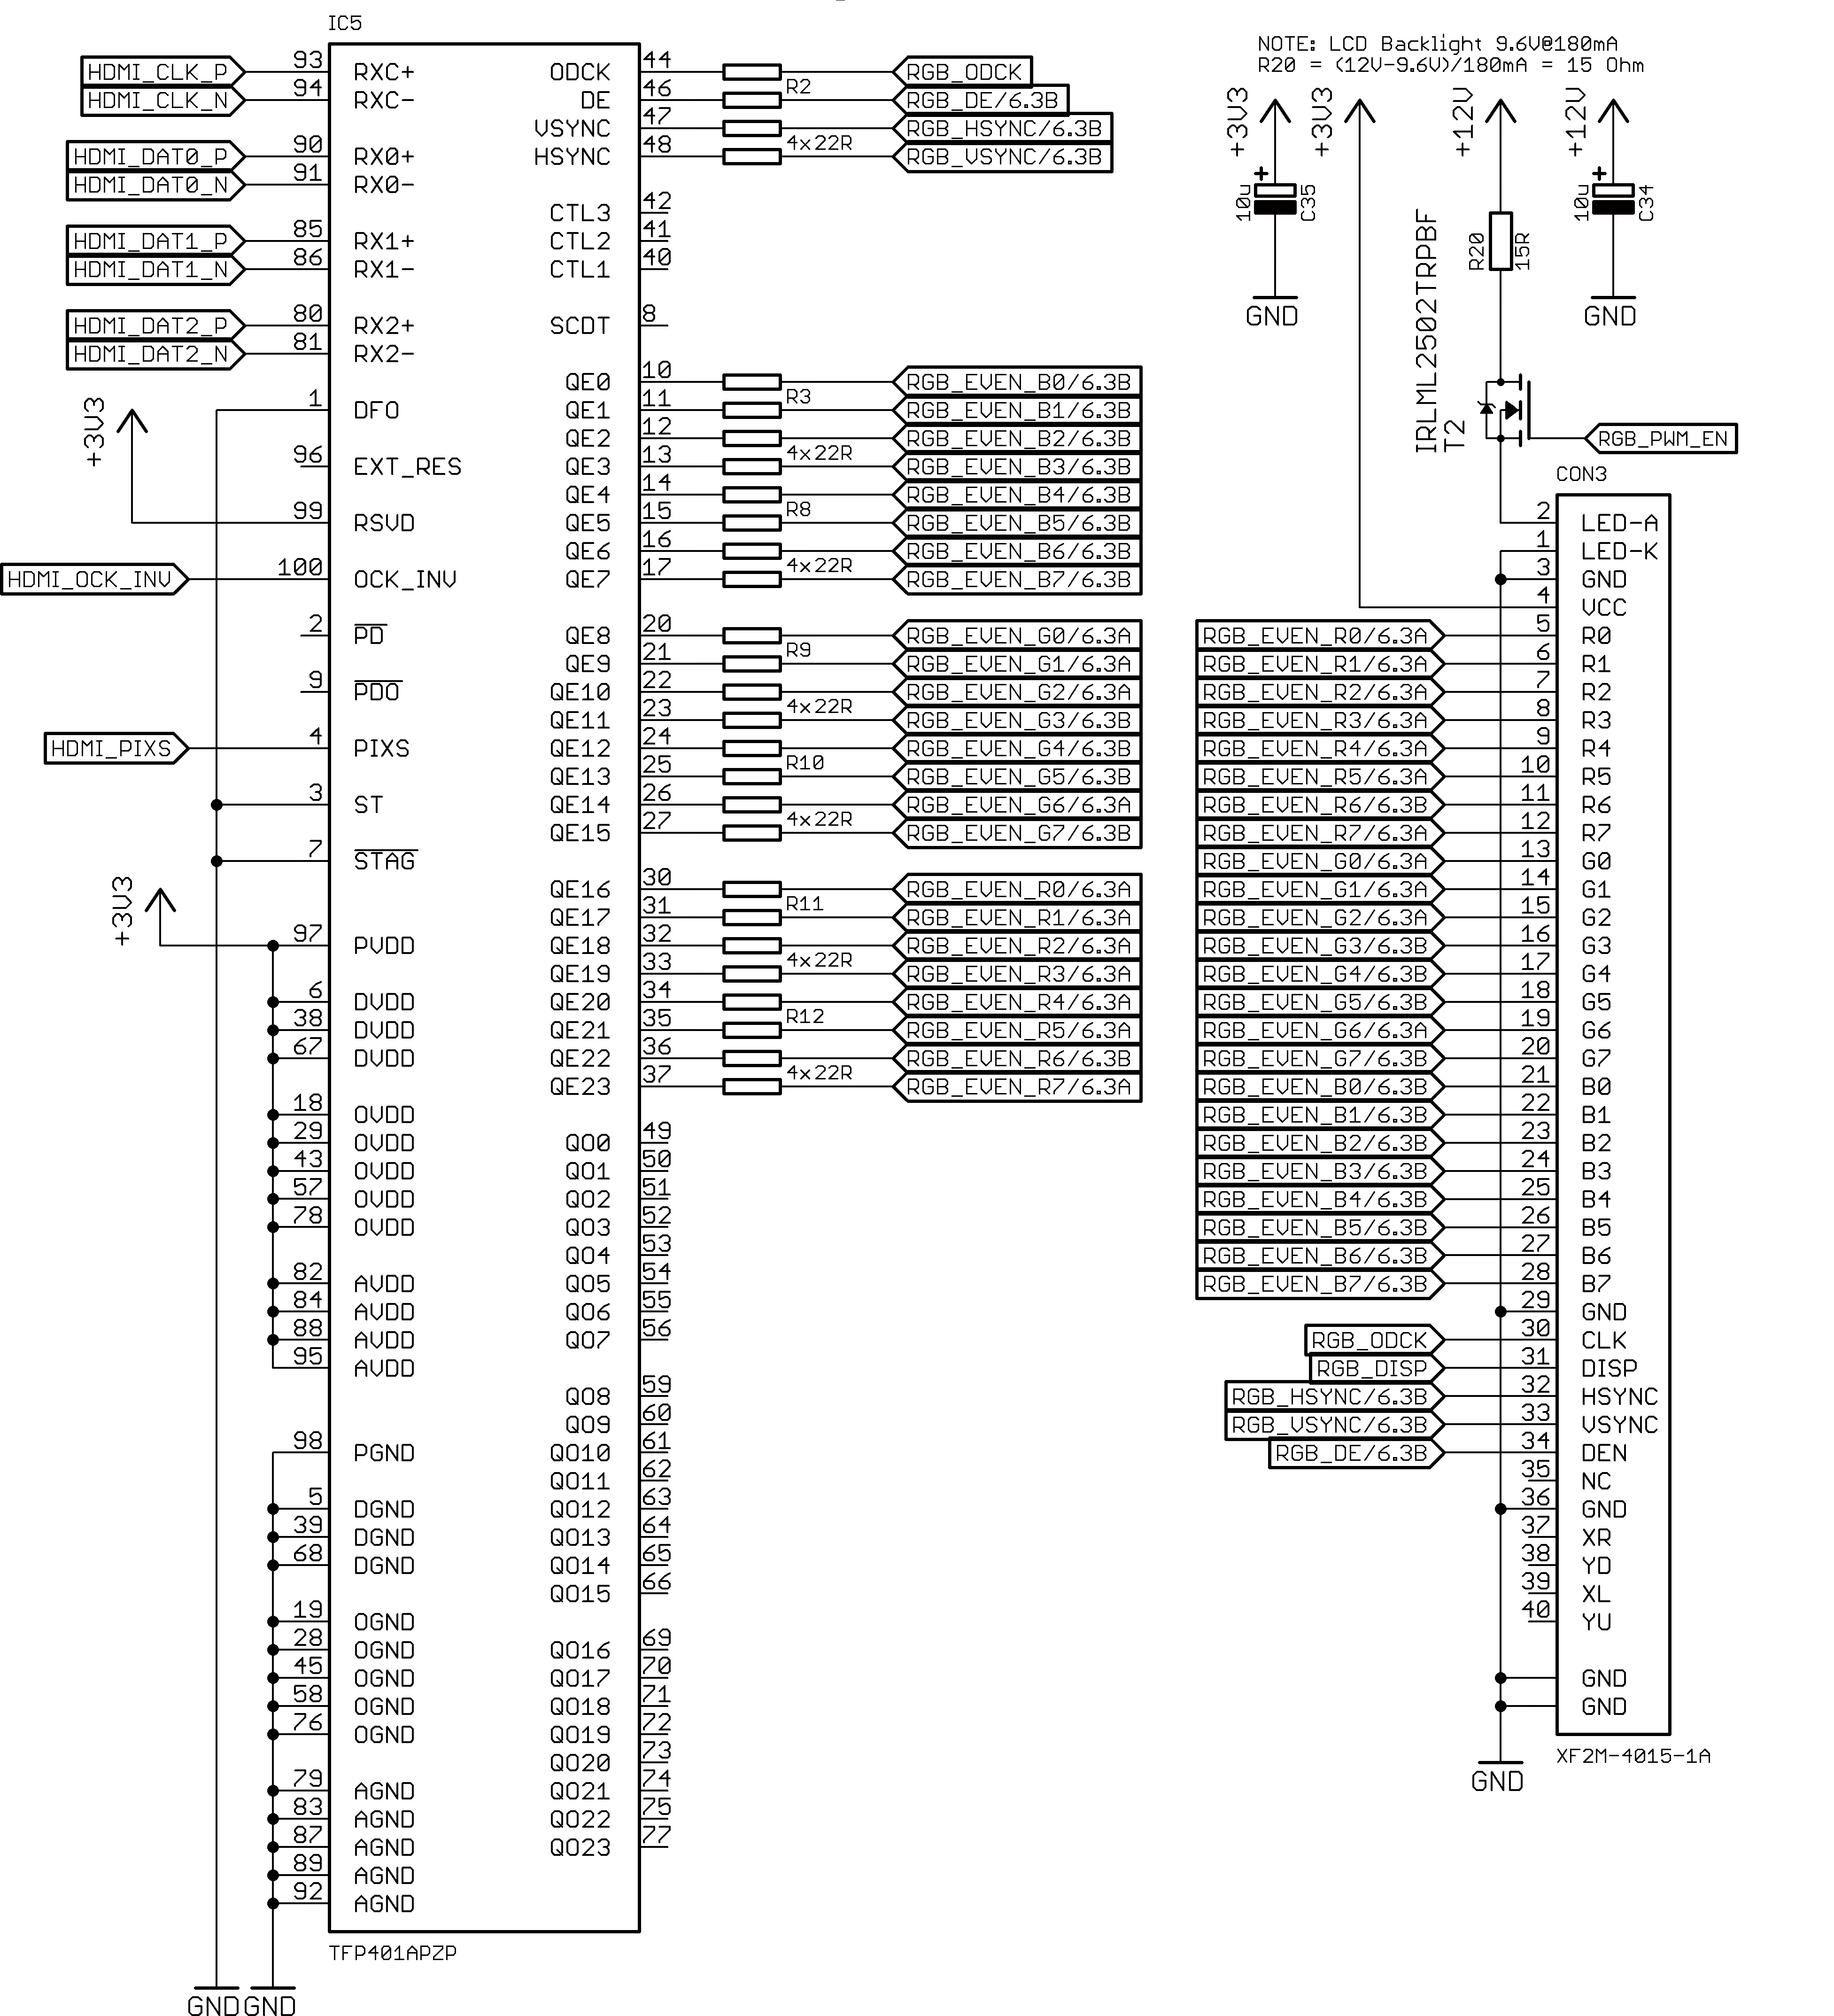
\includegraphics[width=8.5cm,keepaspectratio]{TeilB/rgb_bridge_sch.png}}
        \caption{LVDS Bridge: Schaltplan}
       \label{fig:teilb_lvds_bridge_sch}
\end{figure}\\
Wie auch bei den HDMI-Leitungen muss beim Layouten ein besonderes Augenmerk geworfen werden. Da hier ebenfalls eine Impedanz von 100\,$\Omega$ gefordert werden, sind dieselben Parameter bzgl. Leitungsbreite und Abstand wie in Abschnitt \ref{cha:hdmi_eingang} verwendet, bei der sich eine differentielle Impedanz von 106\,$\Omega$ errechnet.  Die Terminierung findet am Ende der LVDS-Leitungen im Display statt und bedarf keiner zusätzlichen Bauteile auf der Platine. Wie zuvor ist die Länge der Leitungspaare zueinander enorm wichtig. Die Längen der Leitungspaare sind im Bereich zwischen 13.825\,mm und 14.010\,mm, was einer maximalen Abweichung von 1.34 \% entspricht. Durch die angepasste differentielle Impedanz und gleichlangen Leitungen, ist die LVDS-Strecke hinreichend gut dimensioniert. \refa{fig:teilb_lvds_bridge_pcb} zeigt das Layout der LVDS-Bridge. Um die RGB-Signale vom Top-Layer auf den Bottom-Layer zu bekommen, werden diese mit Vias\footnote{Via: Durchkontaktierung} verbunden. Um große Umwege für Rückströme zu verhindern, ist zwischen den Durchkontaktierungen ausreichend Platz, sodass die Vias vollständig von einer Ground-Fläche umschlossen werden.
\begin{figure}[htp]
		\center
		\fbox{	\includegraphics[width=0.6\textwidth,angle=90]{TeilB/lvds_bridge_pcb.png}}
%			\fbox{	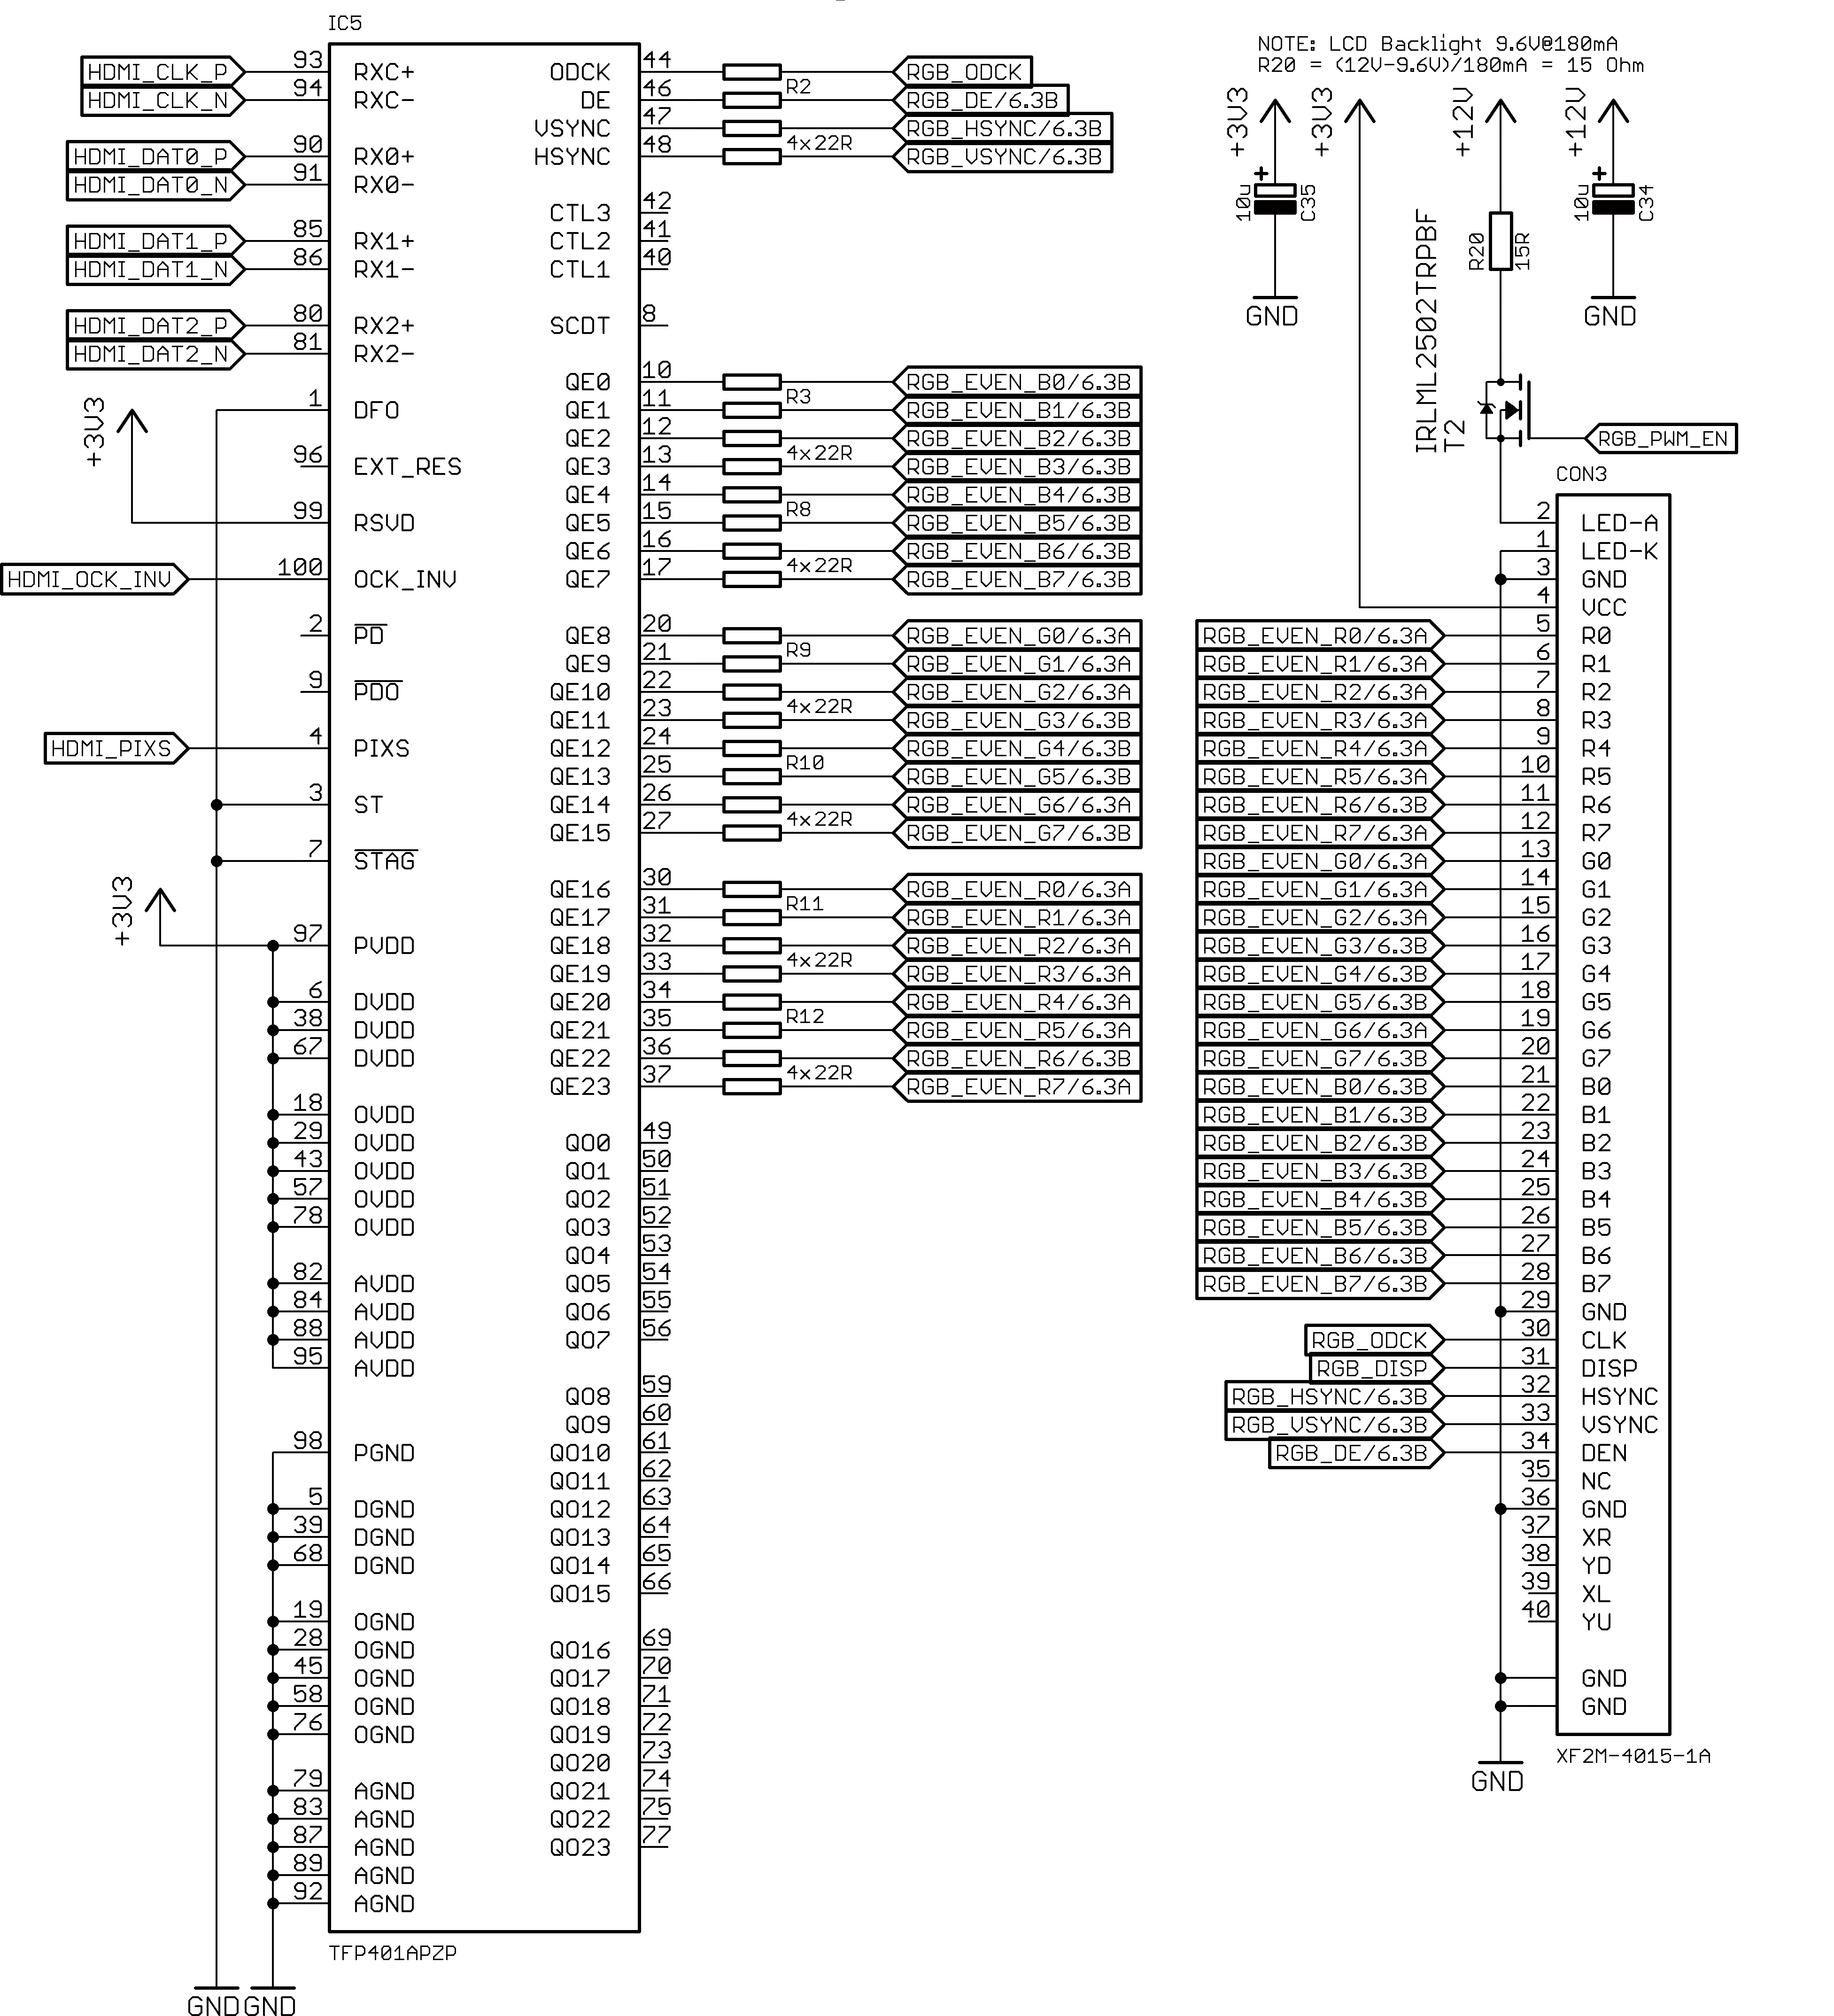
\includegraphics[width=8.5cm,keepaspectratio]{TeilB/rgb_bridge_sch.png}}
        \caption{LVDS Bridge: Layout, gedreht um 90$^{\circ}$}
       \label{fig:teilb_lvds_bridge_pcb}
\end{figure}
\newpage
\subsection{EDID-Daten}
\label{cha:sw_edid_daten}
Wie bereits in \refc{sec:TeilB_Konzept} angesprochen ist ein EEPROM vorhanden, welches die EDID-Informationen beinhaltet. Ohne diese Informationen ist ein Plug-And-Play-Betrieb der Hardware an einer HDMI-Quelle nicht möglich, da der Quelle nicht mitgeteilt wird, welche Randbedingungen an Timings und Auflösung das Anzeigegerät benötigt. Um den Anschluss von verschiedenen RGB- oder LVDS-Displays zu gewährleisten, können die EDID-Daten über eine integrierte USB-Buchse und dem zugehörigen Programm direkt auf der Hardware programmiert werden. \refa{fig:teilb_edid_blockschaltbild} zeigt einen Ausschnitt aus \refa{fig:teilb_architektur}, das die einzelnen Komponenten des EDID-Blocks darstellt. 
\begin{figure}[htp]
	\center
	\fbox{	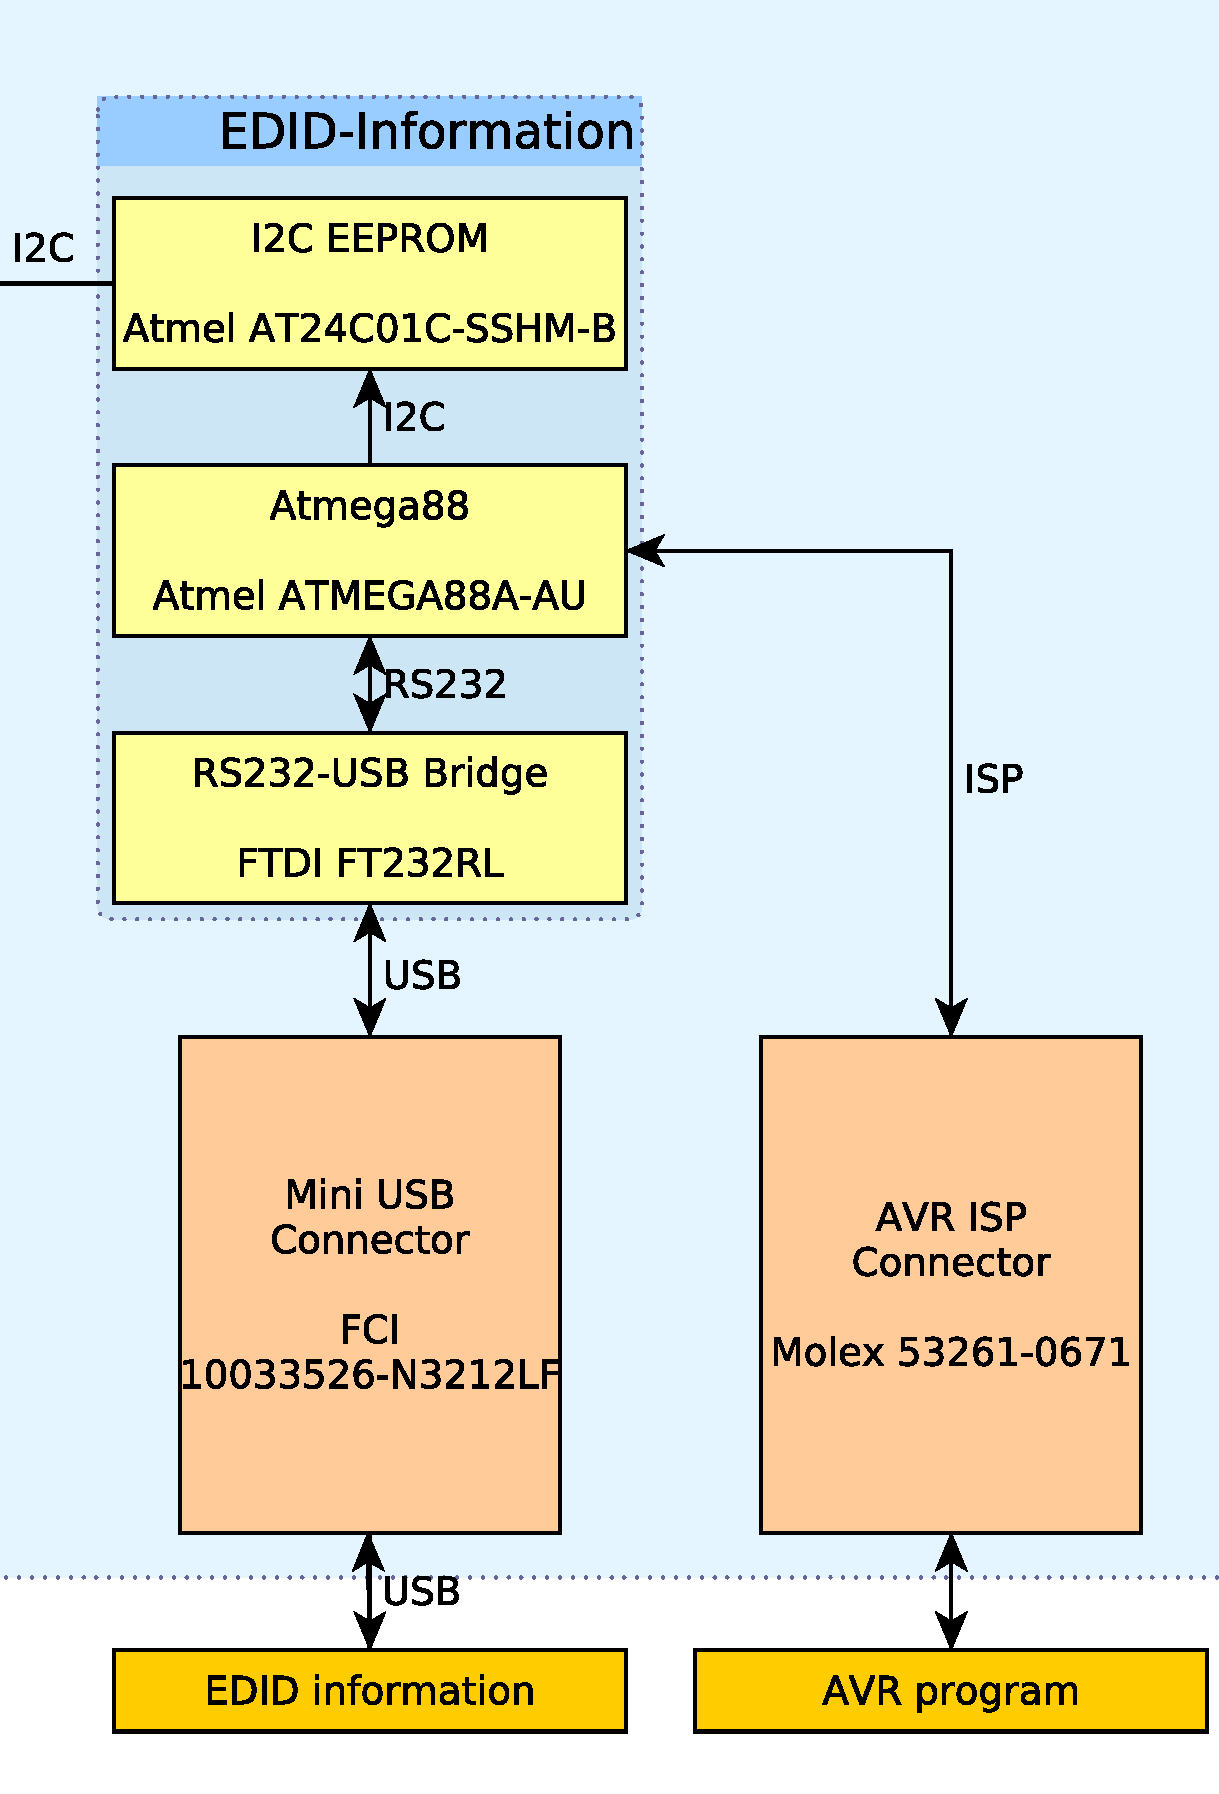
\includegraphics[width=0.6\textwidth]{TeilB/EDID.pdf}}
    \caption{EDID: Blockschaltbild}
    \label{fig:teilb_edid_blockschaltbild}
\end{figure}\\
Als externe Schnittstellen stehen eine USB-Buchse und ein ISP-Stecker\footnote{ISP: In System Programmer - Schnittstelle um den Prozessor im eingebauten Zustand zu programmieren} für den Prozessor zur Verfügung. Die RS232-UART-Bridge stellt die Kommunikation mit dem PC her, indem diese die serielle Schnittstelle des AVRs in USB-Signale umwandelt. Dies ist notwendig, da heutzutage kaum mehr echte serielle Schnittstellen in Computern verbaut sind. Gerade im embedded Bereich ist die Verwendung der seriellen Schnittstelle aufgrund seiner einfachen Bedienung sehr beliebt, weshalb Lösungen mittels USB-Konvertern quasi zum Standard gehören. Der Prozessor selbst ist durch einen ATMEGA88 realisiert, und beschreibt das $I^2C$-EEPROM mit einem in der Software hinterlegten Protokoll. 
\refa{fig:teilb_edid_usb_sch} zeigt die USB-Bridge mit dem USB-Stecker und dem Baustein \code{FT232RL} von FTDI, der die Konversion durchführt. Die differentiellen USB-Signale \code{USB_D+} und \code{USB_D-} sind mit dem Eingang des Bausteins verbunden. An den Ausgängen sind die seriellen Signale \code{FTDI_RX} und \code{FTDI_TX}. Diese Leitungen stellen die ein- beziehungsweise ausgehenden Signale zum und vom Prozessor dar.
\begin{figure}[htp]
	\center
	\fbox{	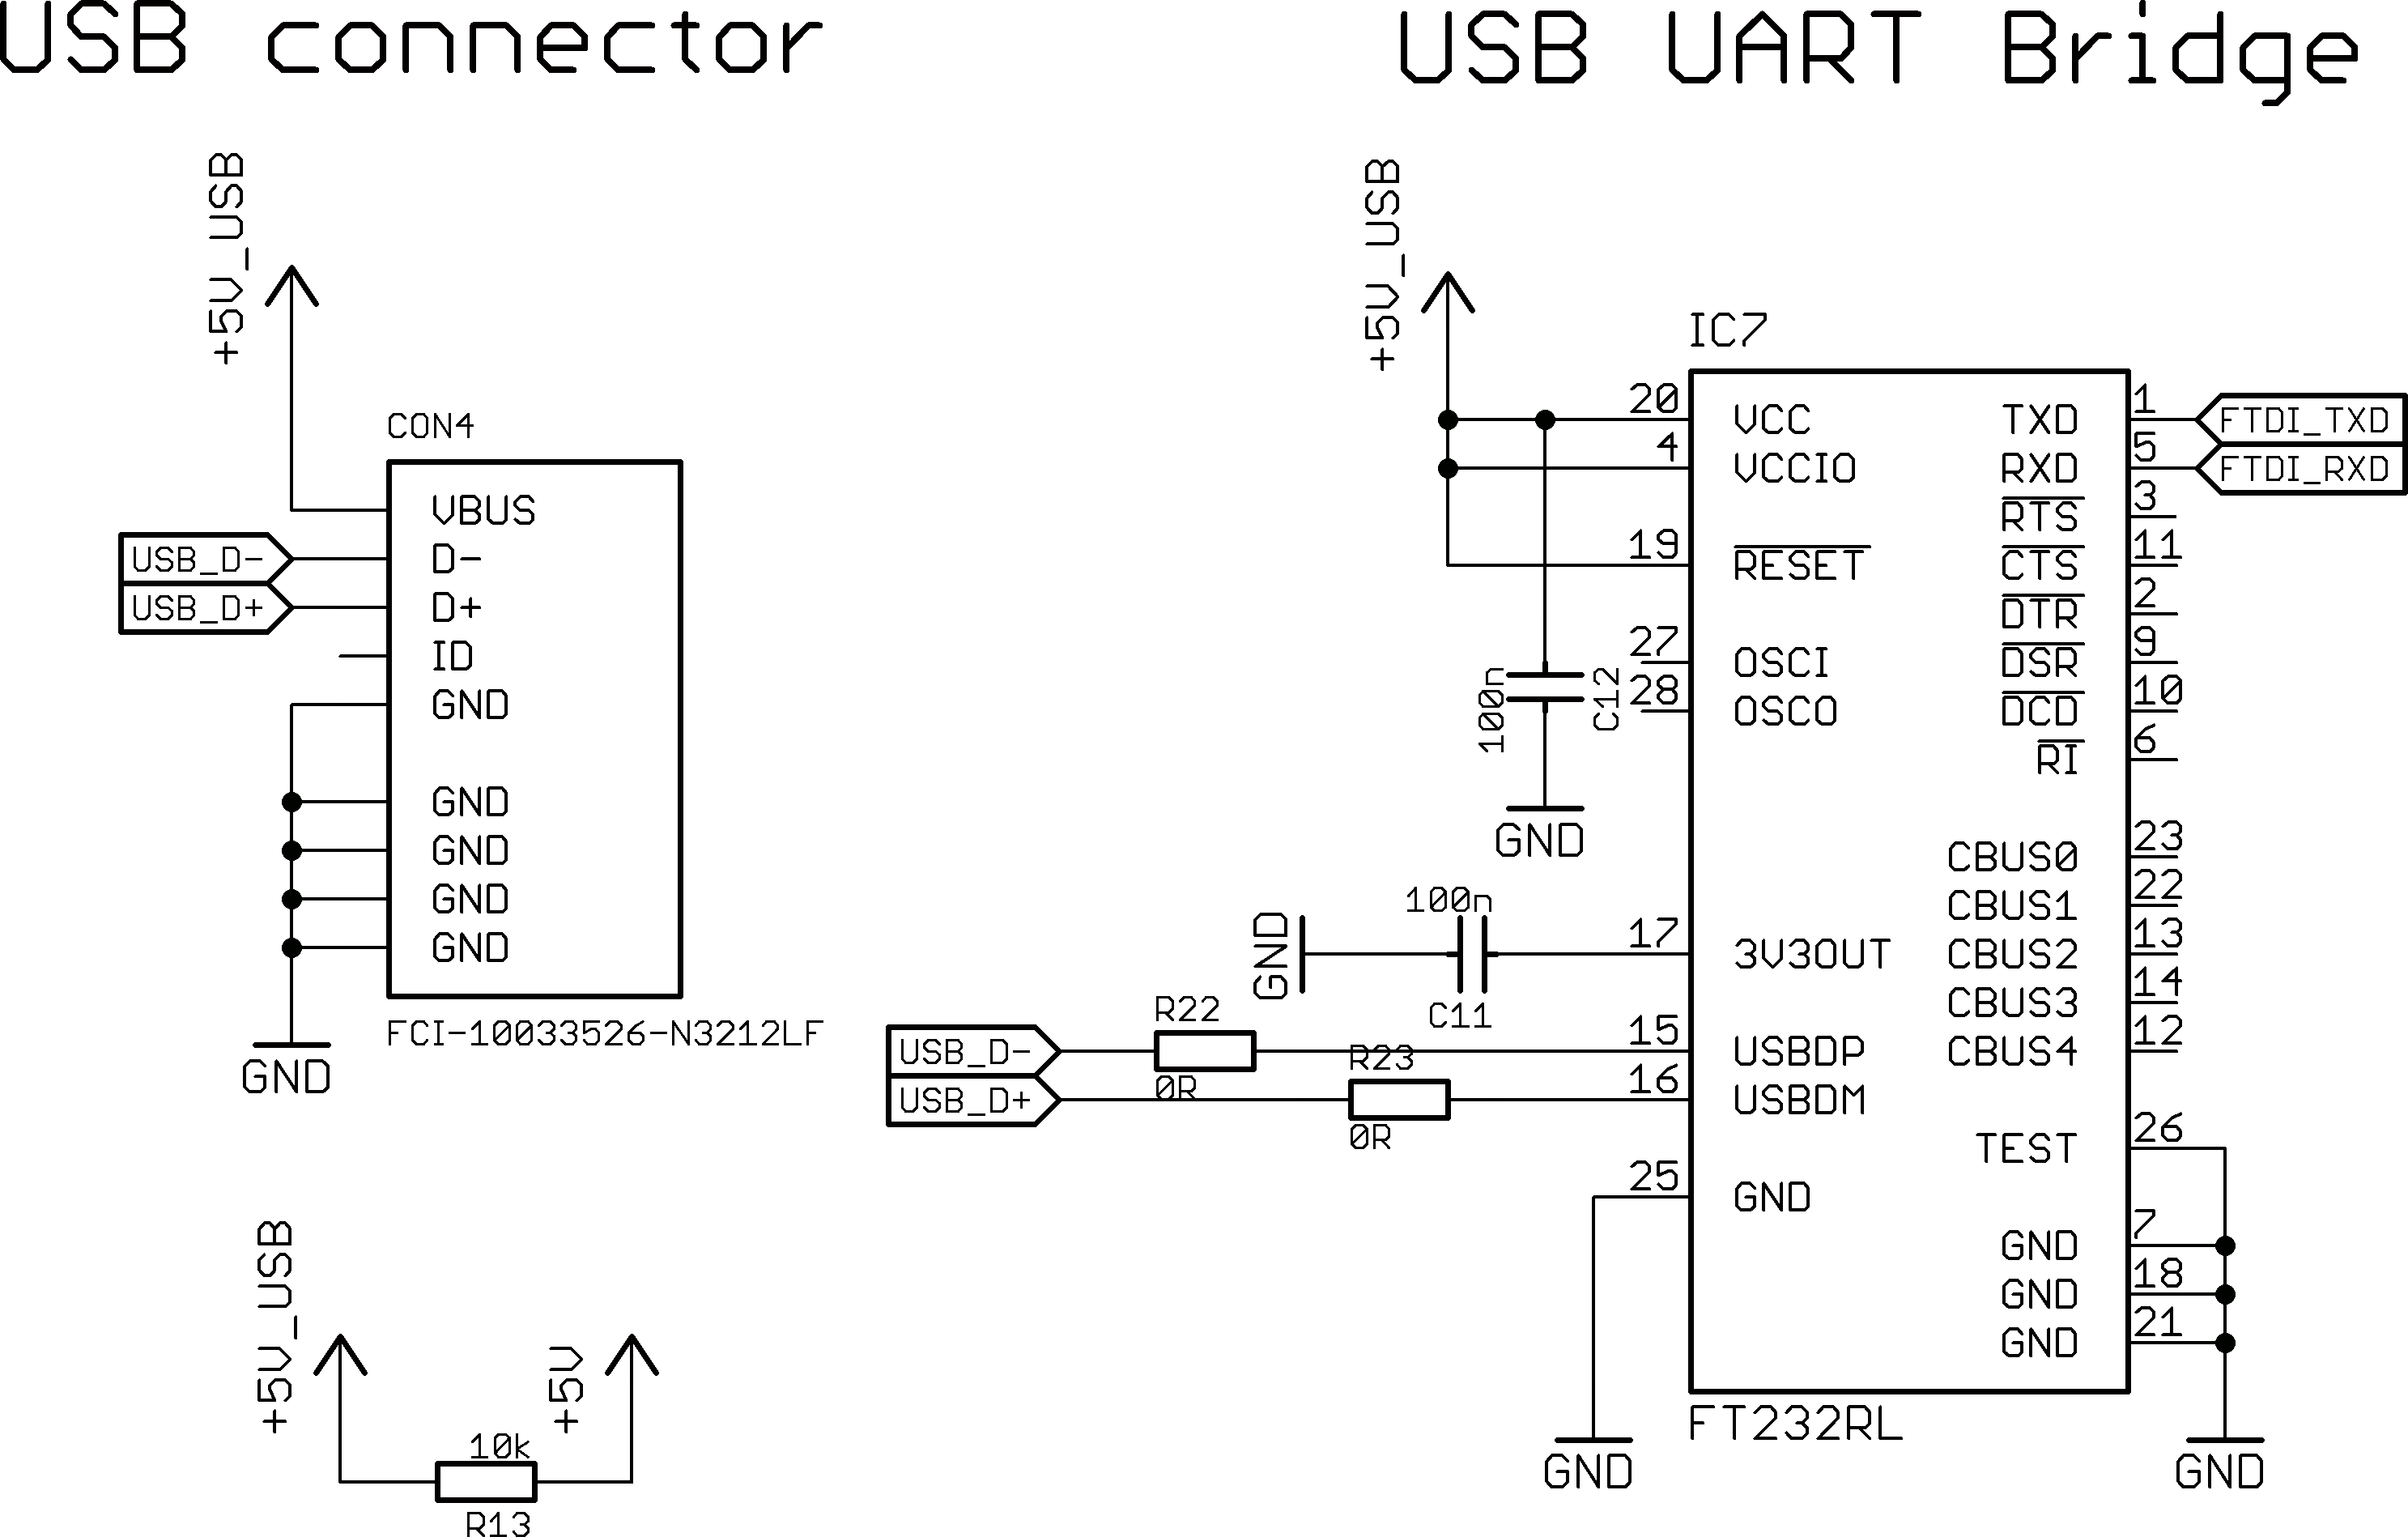
\includegraphics[width=0.8\textwidth]{TeilB/usb_sch.png}}
    \caption{EDID: USB-Bridge Schaltplan}
    \label{fig:teilb_edid_usb_sch}
\end{figure}\\
\refa{fig:teilb_edid_avr_sch} zeigt die Beschaltung des AVRs \code{IC6} und des EEPROMs \code{IC4}. Neben der Grundbeschaltung mit Quarz und Reset-Pin am AVR gehen die $I^2C$-Signale \code{EDID_SCL} und \code{EDID_SDA} an die Pins des EEPROMs. Das EEPROM bietet die Möglichkeit einen Schreibschutz aktiv zu schalten. Dieser kann mit dem Jumper \code{JP5} ein- und ausgeschaltet werden. Zum Programmieren des Prozessors ist der ISP-Stecker mit den entsprechenden Signalen verbunden. Um die Bauform recht gering zu halten sind alle Komponenten als SMD-Varianten gewählt - so auch der ISP-Stecker \code{CON5}. Um die 128 Byte großen EDID-Daten vollständig aufnehmen zu können ist das entsprechend gleichgrosse EEPROM \code{AT24C01C} in Verwendung. \\
Neben der reinen Funktion als Programmiergerät für das EEPROM bietet die Schaltung noch die Möglichkeit ein PWM-Signal auszugeben, welches zum Dimmen der Hintergrundbeleuchtungen der Displays verwendet werden kann. Hierzu ist ein Potentiometer mit dem Signal \code{AVR_PWM_ADC} an einem Analog-Eingang des AVRs verbunden, der es ermöglicht die Spannung im Bereich zwischen +5V und 0V zu messen. Je nach gemessener Spannung am Potentiometer kann ein PWM-Signal \code{AVR_PWM} ausgegeben werden, wobei beispielsweise +5\,V 100\%  und +2.5\,V 50\% Helligkeit bedeuten. Liegen 0V am Eingang an, so wäre die Hintergrundbeleuchtung komplett ausgeschaltet, wobei sich das PWM-Signal stufenlos im gültigen Wertebereich einstellen lässt. 
\begin{figure}[htp]
	\center
	\fbox{	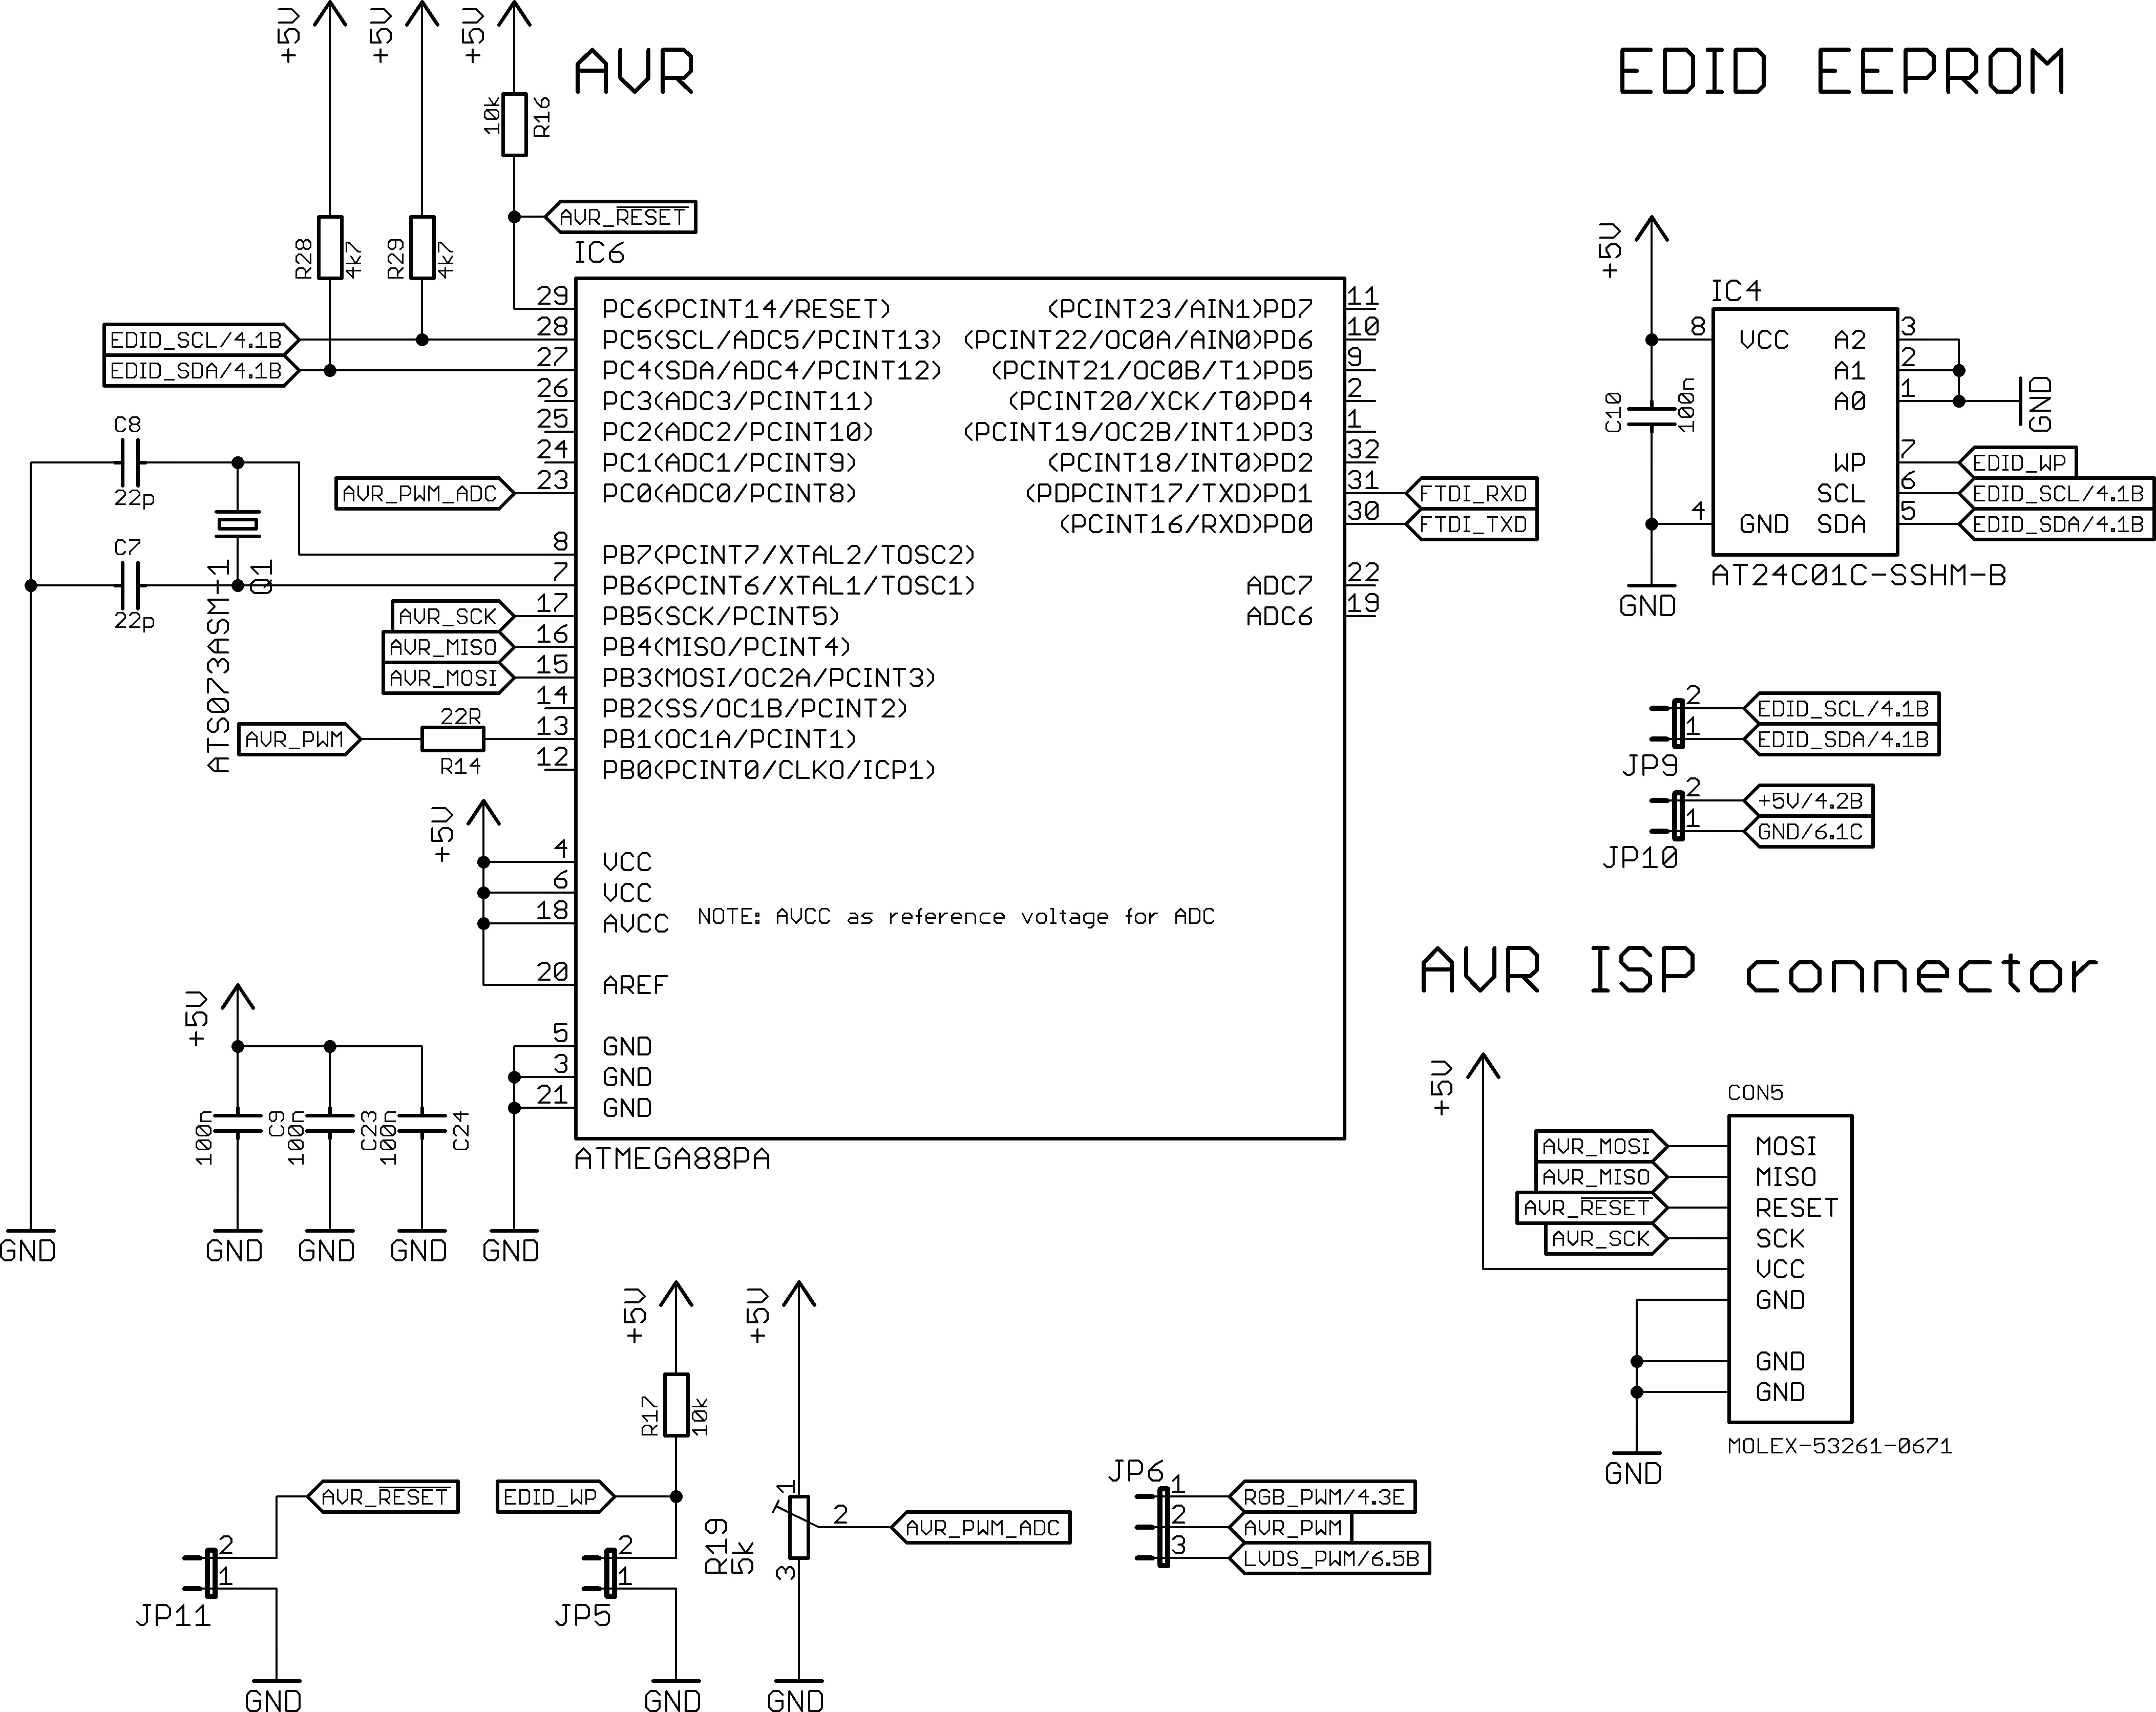
\includegraphics[width=1\textwidth]{TeilB/avr_sch.png}}
    \caption{EDID: AVR Schaltplan}
    \label{fig:teilb_edid_avr_sch}
\end{figure}\\
Der einzige kritische Aspekt beim Layout des Funktionsblocks ist der eingenommene Raum auf der Platine. Da hier weder mit schnellen Signalen noch hohen Strömen gearbeitet wird, kann die Leitungsführung platzoptimiert durchgeführt werden. Die Abbildungen \ref{fig:teilb_edid_pcb_top} und \ref{fig:teilb_edid_pcb_bot} zeigen das Layout auf dem Top- bzw. Bottom-Layer der Platine. In den Bildern sind die einzelnen Bereiche farblich und textuell markiert.

\begin{figure}[htbp]
        %\begin{center}
        \centering
        \begin{subfigure}[htp]{0.48\textwidth}
%                \fbox{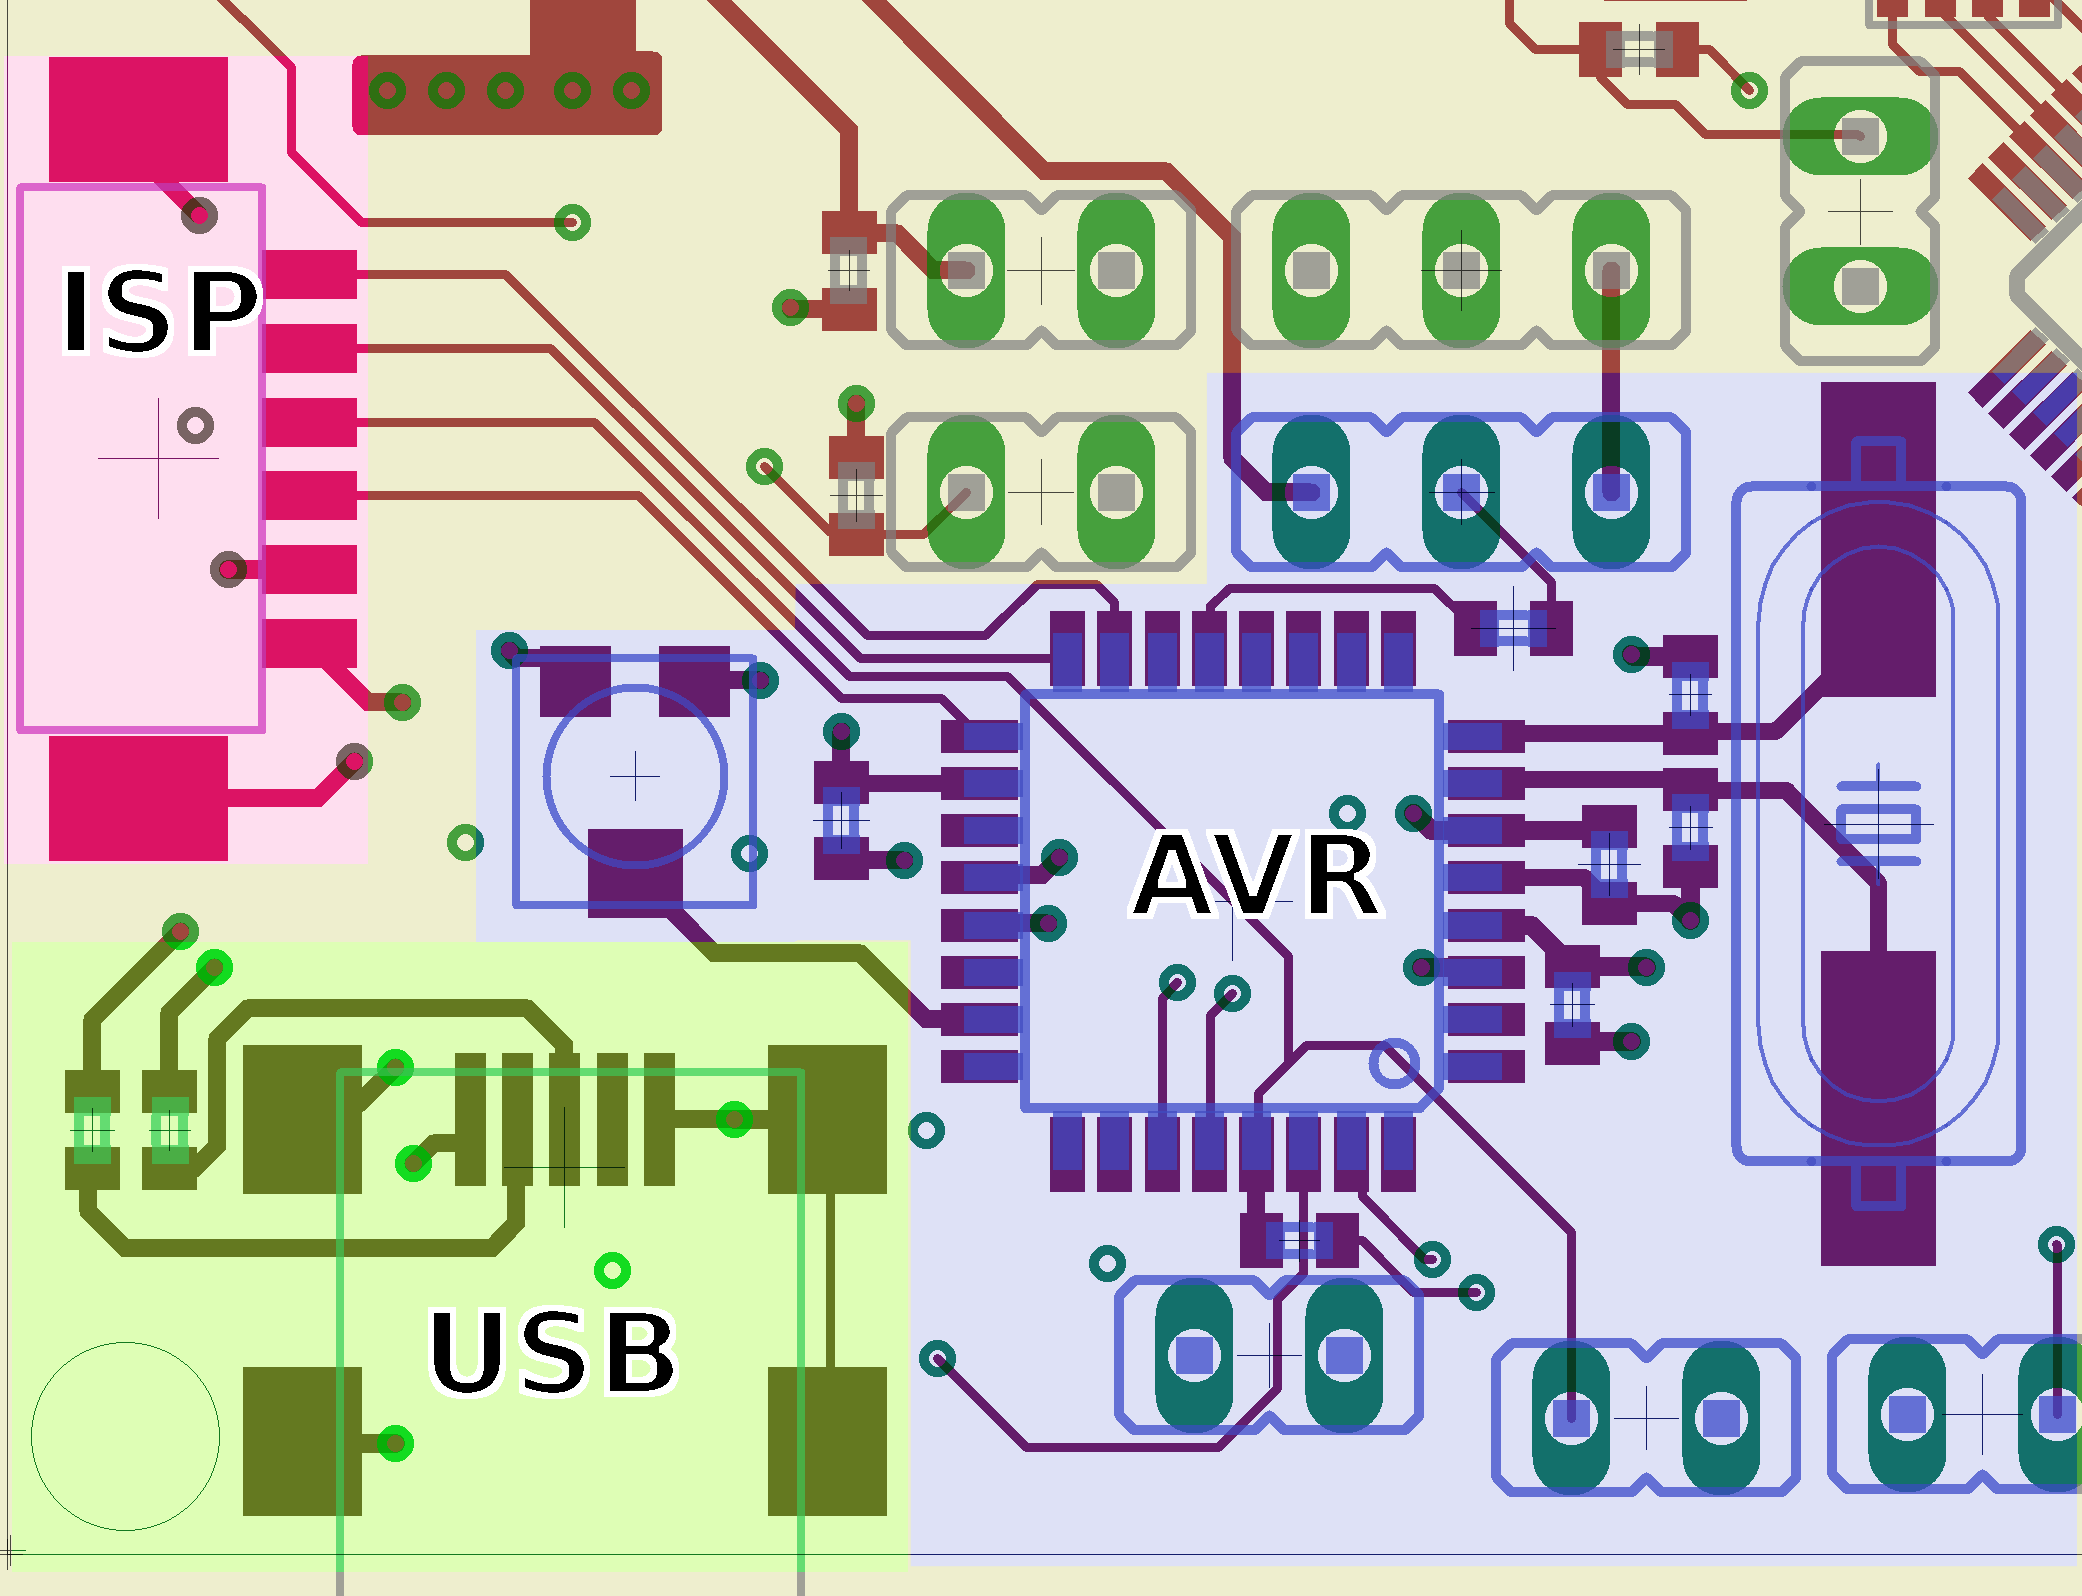
\includegraphics[width=1\textwidth]{TeilB/edid_pcb_top.png}}
                \fbox{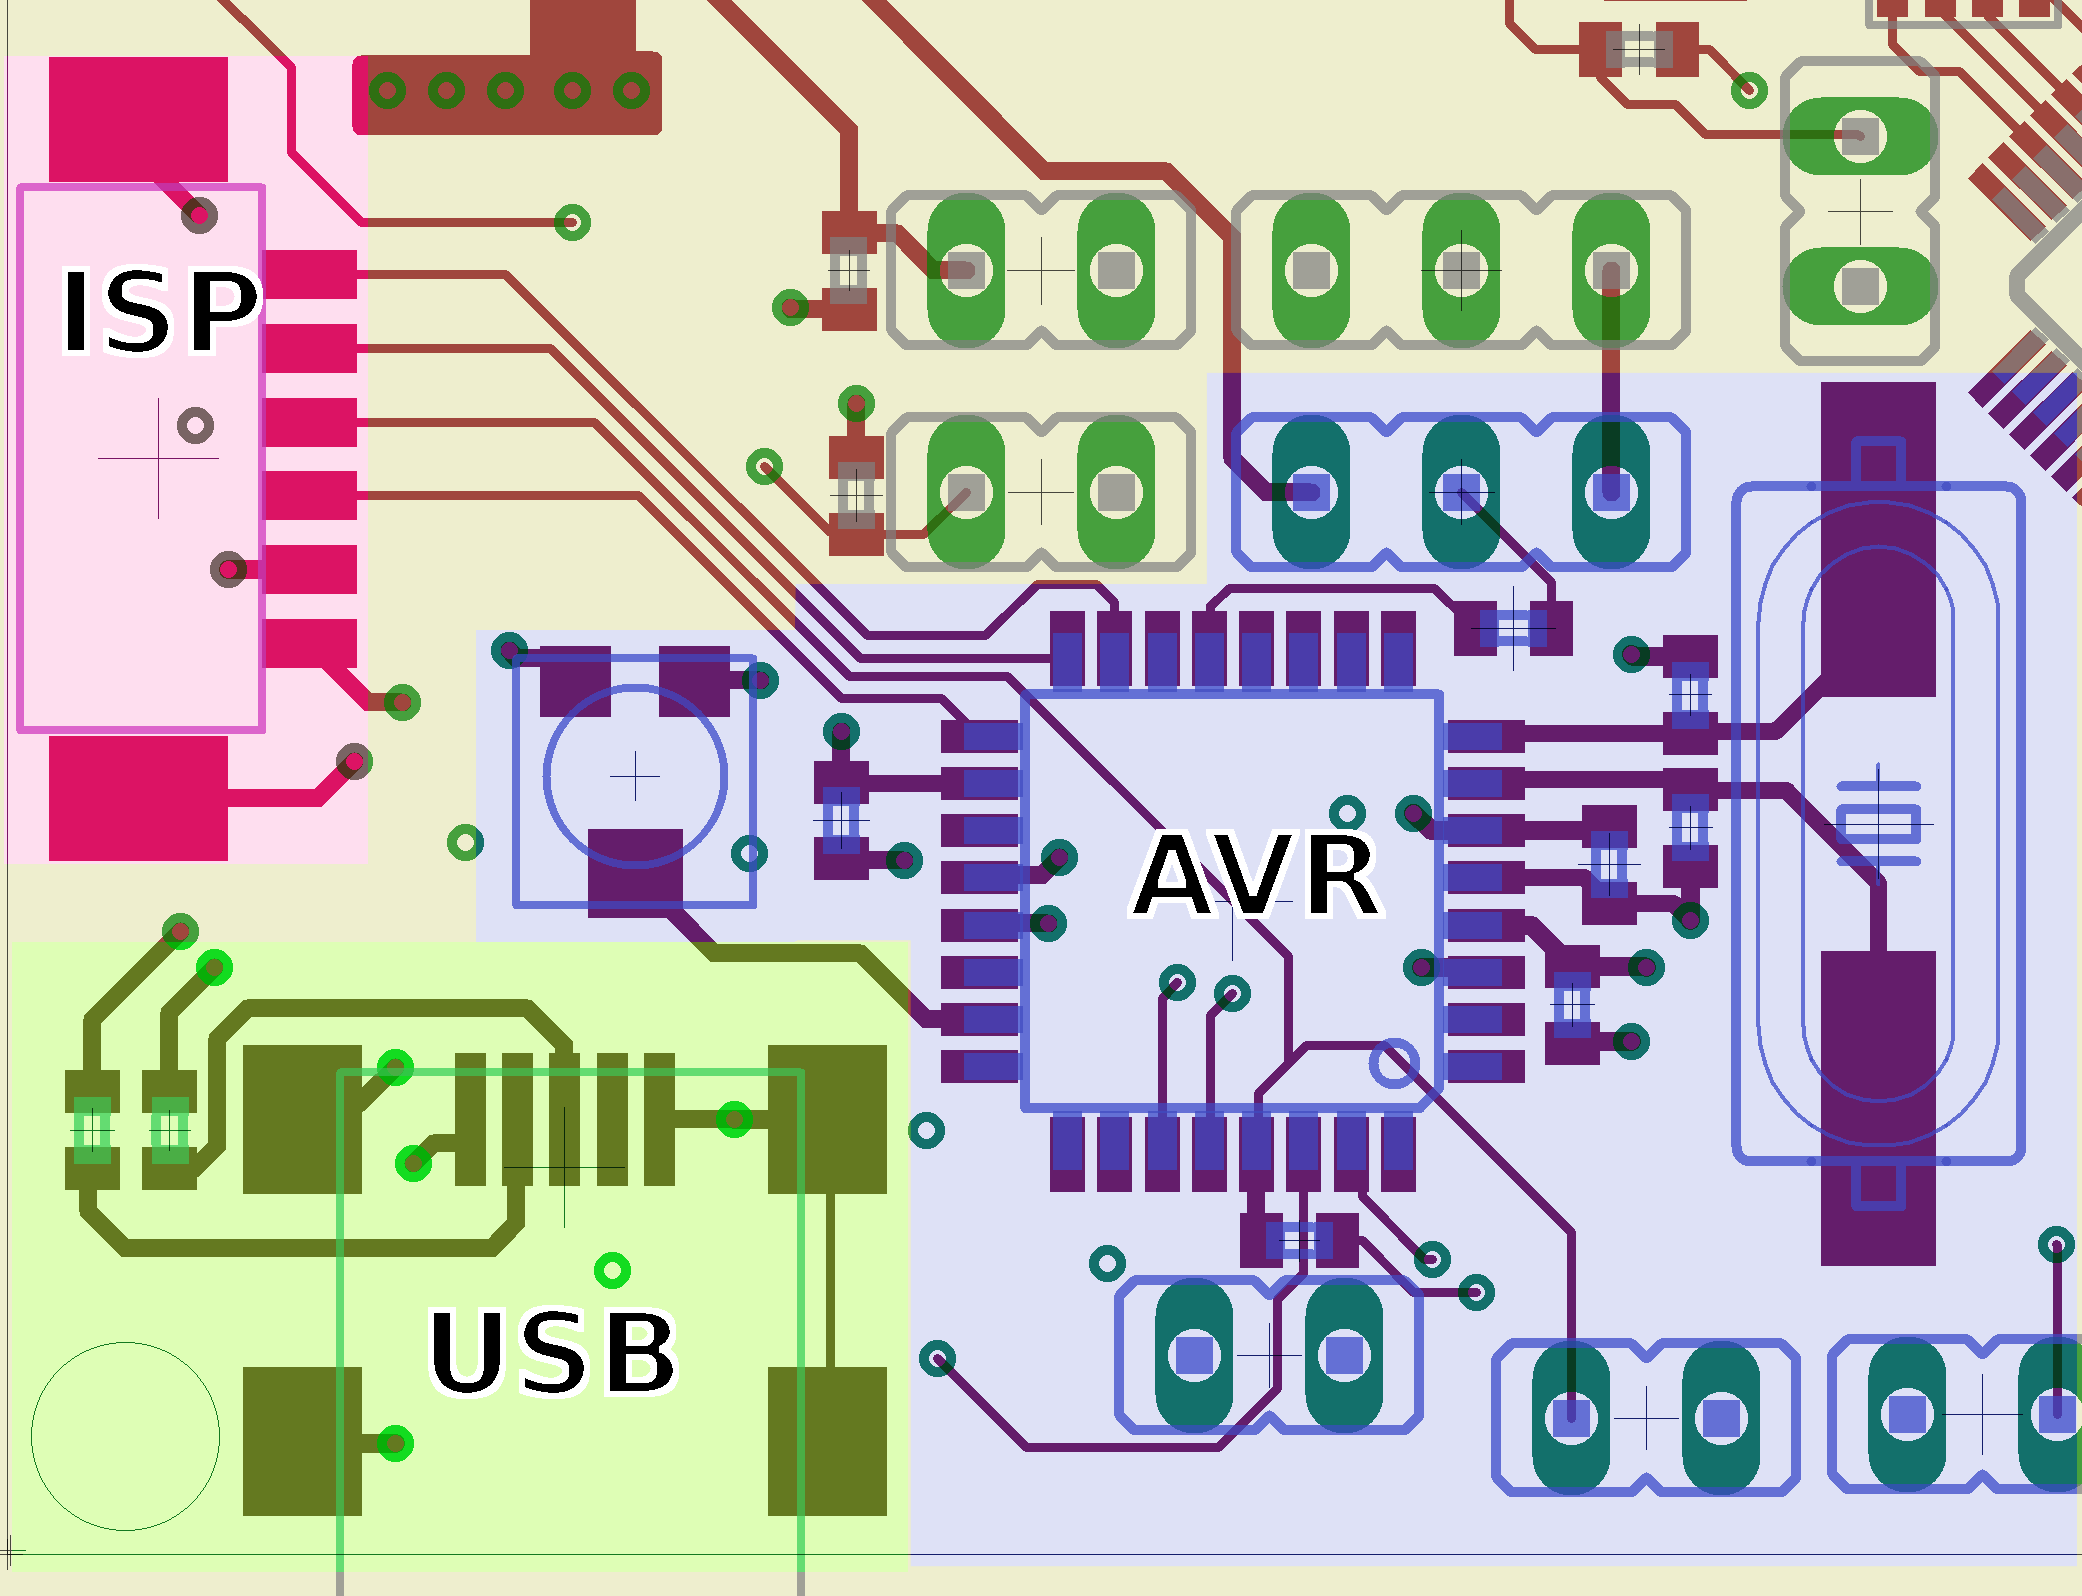
\includegraphics[height=5cm]{TeilB/edid_pcb_top.png}}
                \caption{Top Layer}
                \label{fig:teilb_edid_pcb_top}
        \end{subfigure}
\quad 
        \begin{subfigure}[htp]{0.48\textwidth}
%               \fbox{ 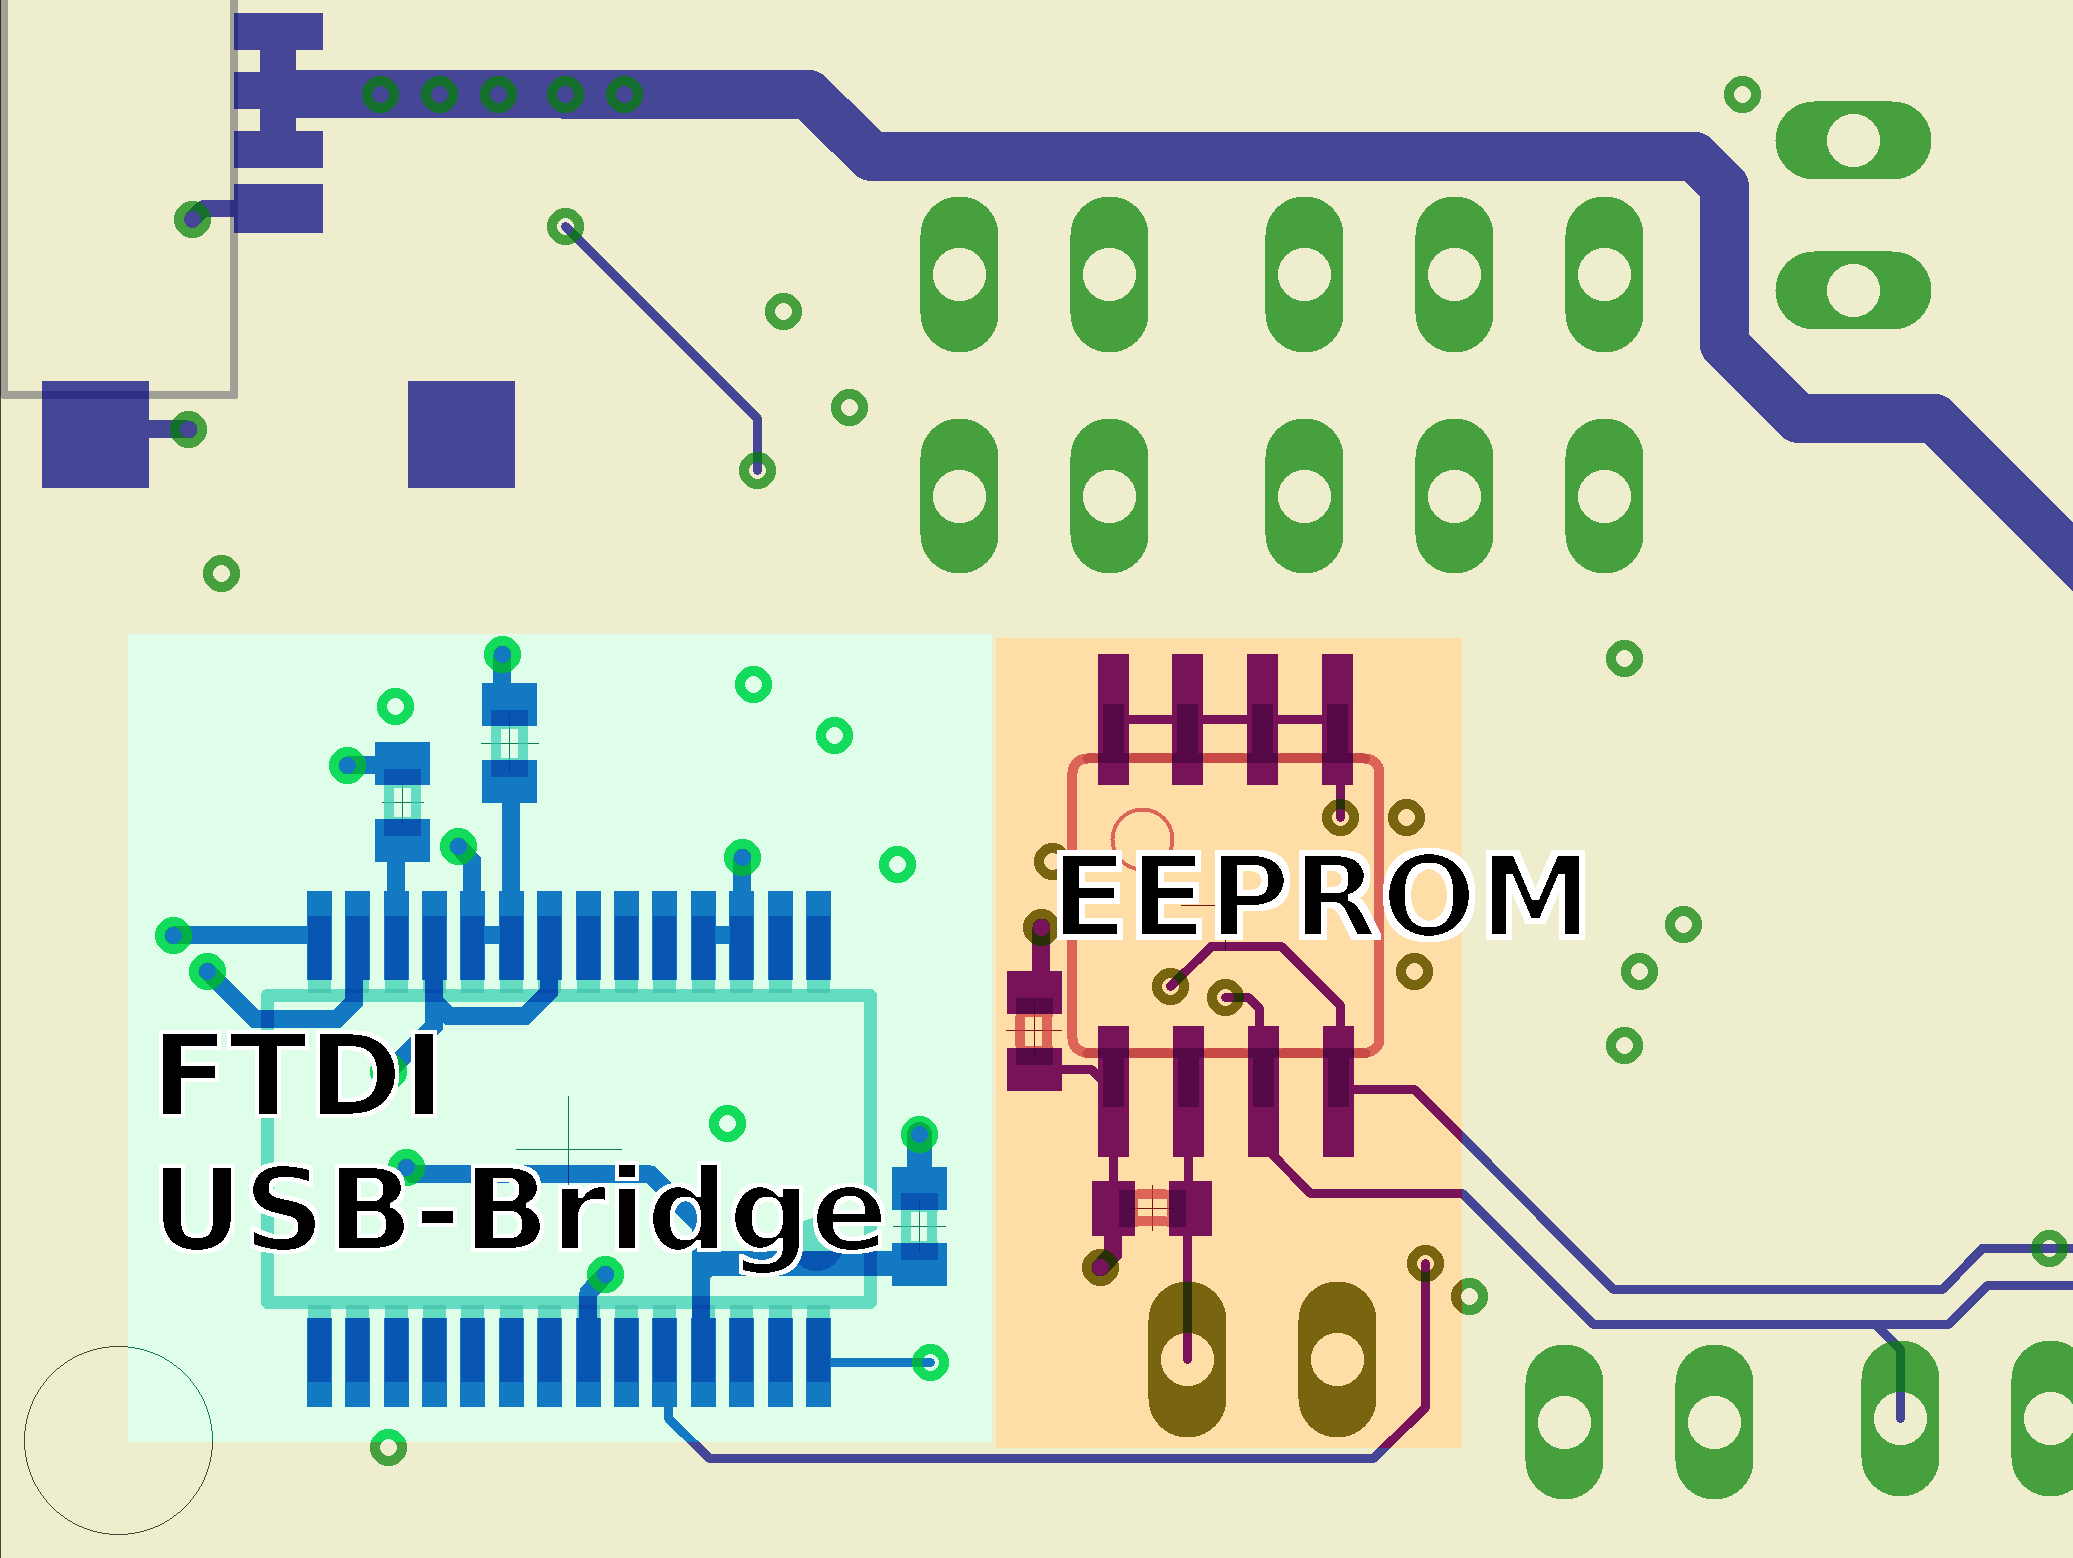
\includegraphics[width=1\textwidth]{TeilB/edid_pcb_bot.png} }              		
               \fbox{ 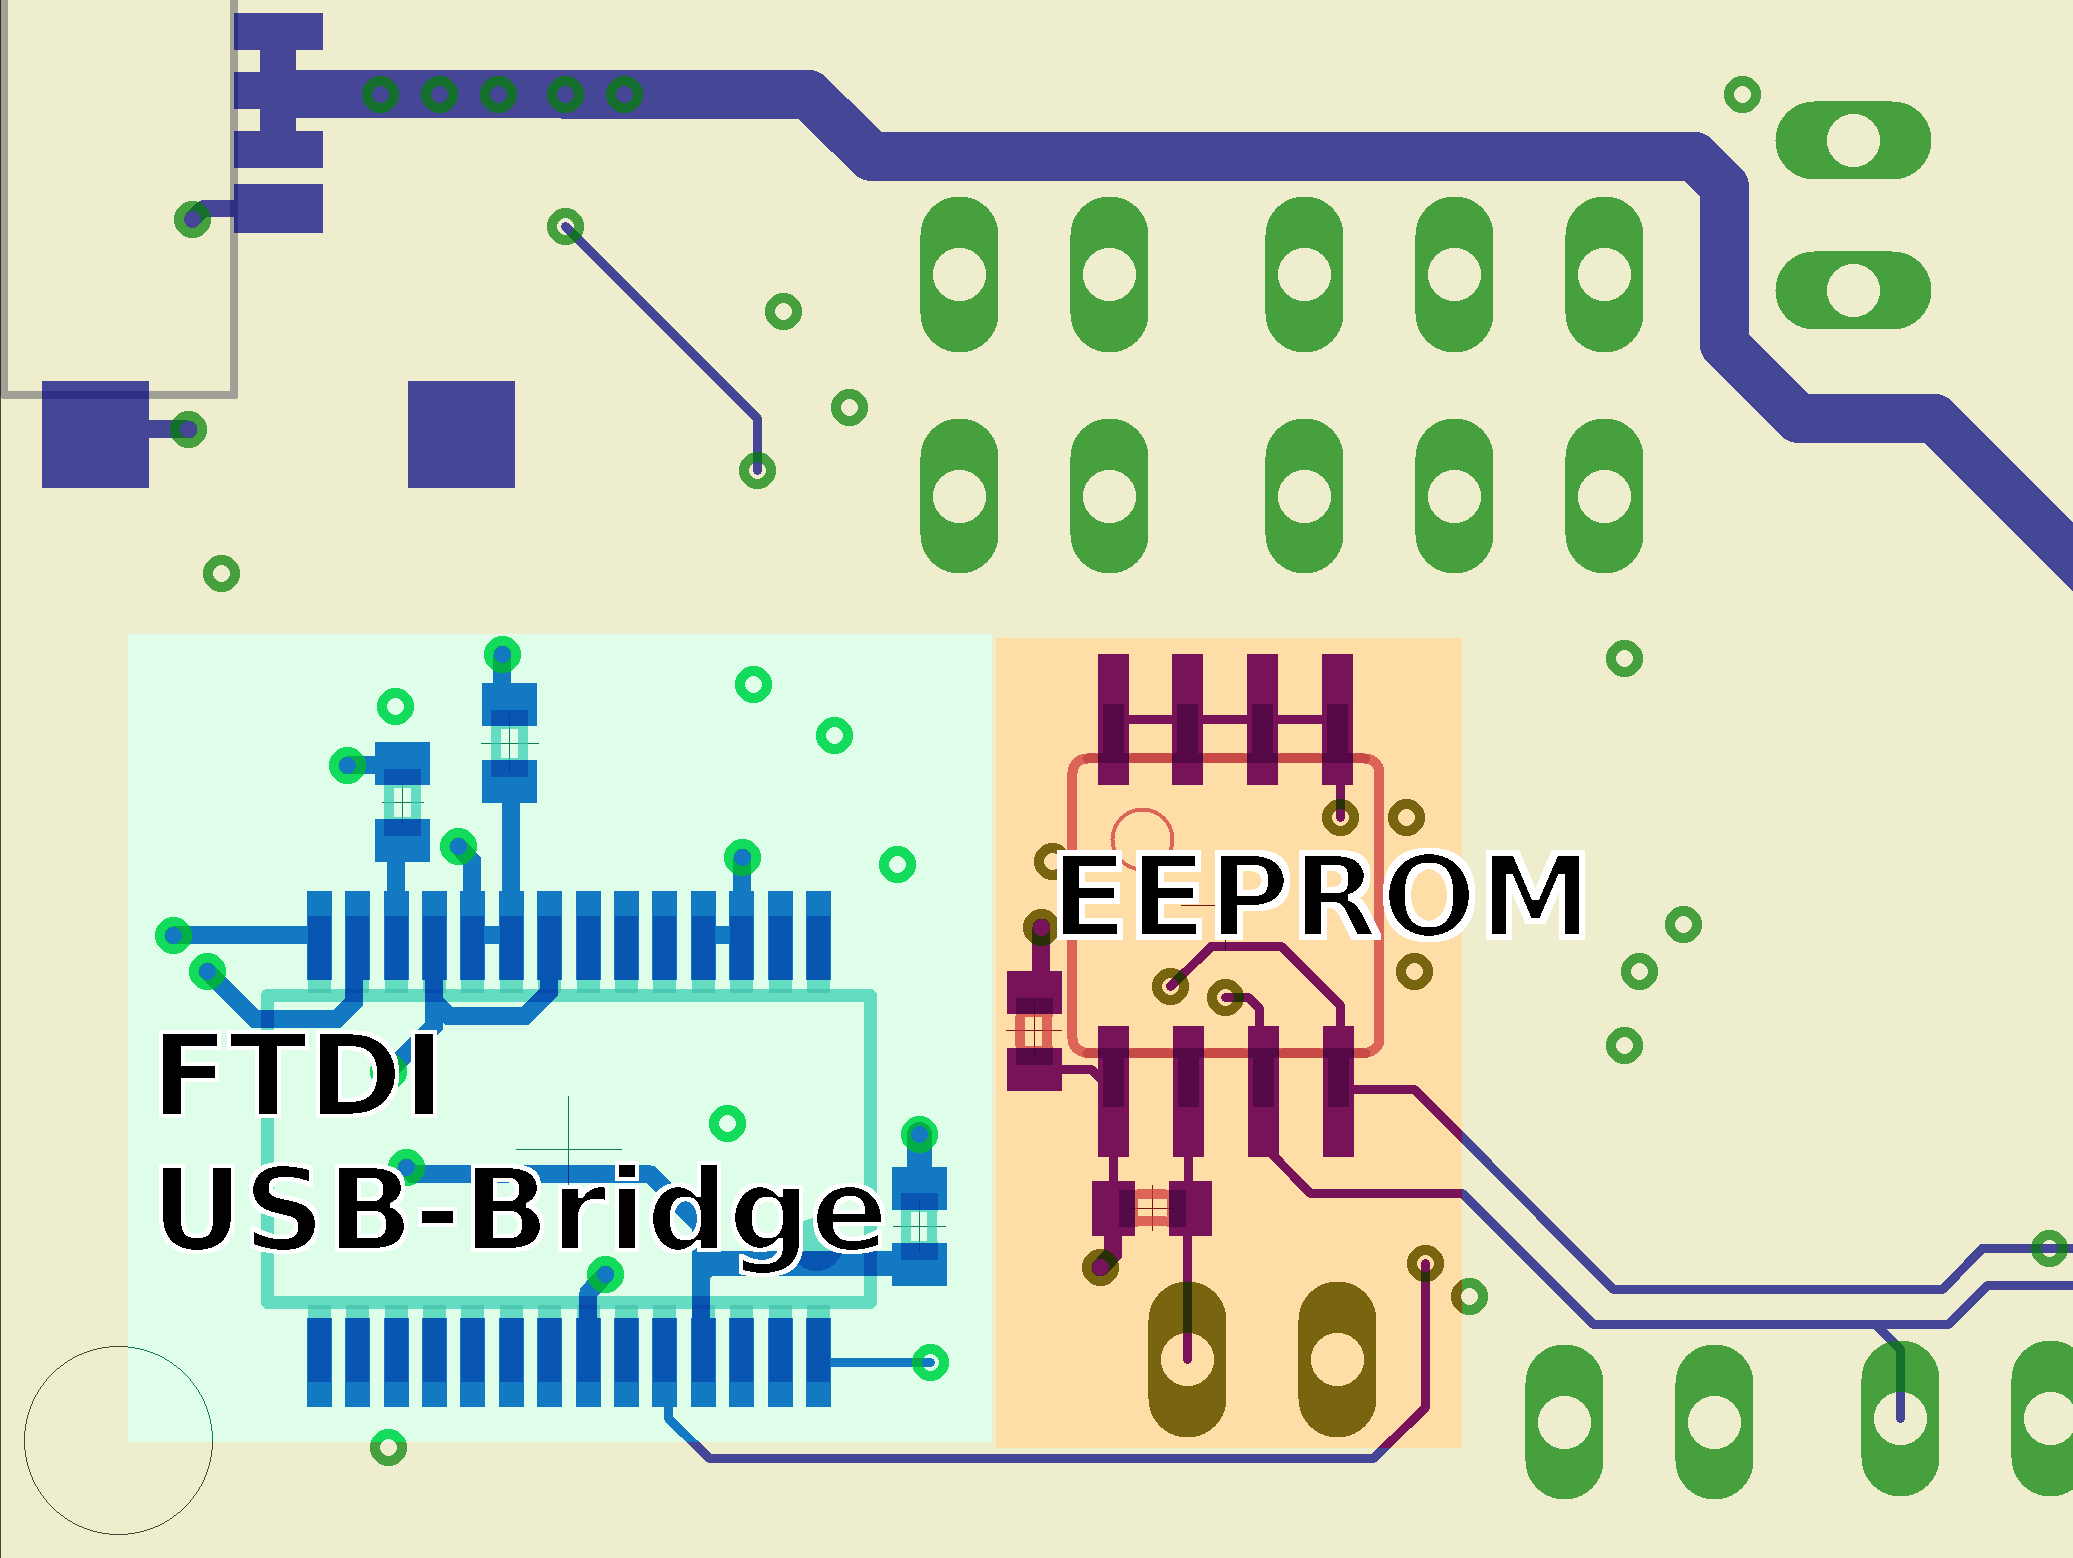
\includegraphics[height=5cm]{TeilB/edid_pcb_bot.png} }              		
		\caption{Bottom Layer}
                \label{fig:teilb_edid_pcb_bot}
        \end{subfigure}
		%\end{center}
        \caption{EDID Baugruppe}
        \label{fig:teilb_edid_pcb}
\end{figure}


\subsection{Spannungsversorgung}
Im Projekt werden drei verschiedene Spannungen verwendet. \refa{fig:teilb_supply} zeigt, wie die Spannungen voneinander abhängen und welche Baugruppe wie versorgt wird. 
\begin{figure}[htp]
	\center
	\fbox{	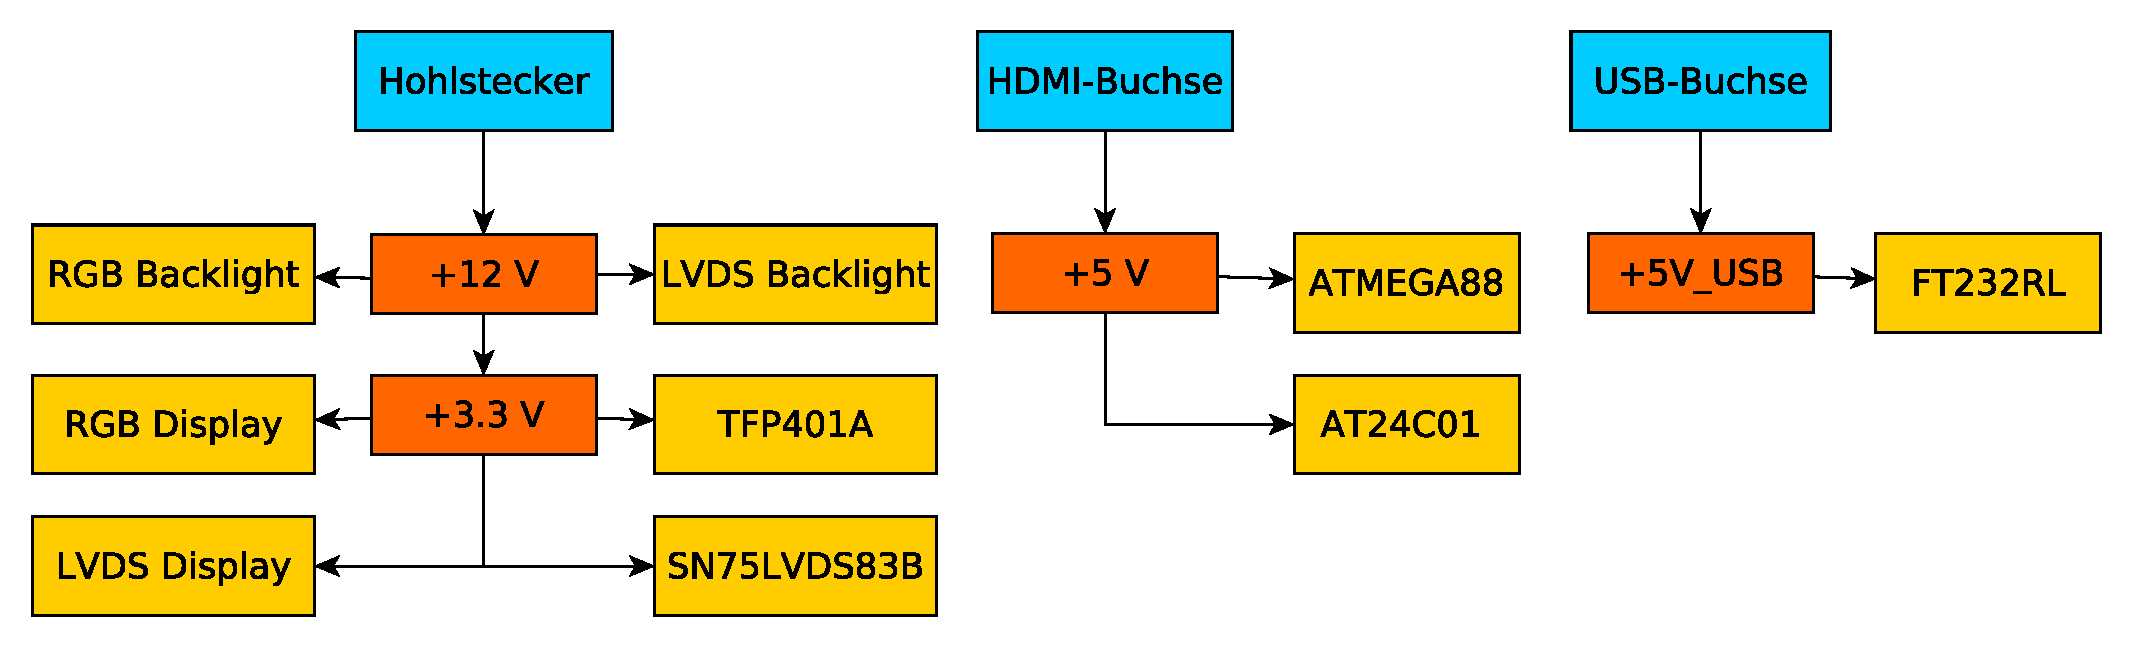
\includegraphics[width=1\textwidth]{TeilB/Supply.pdf}}
    \caption{Spannungsversorgung Teil B}
    \label{fig:teilb_supply}
\end{figure}\\
Extern werden über einen Hohlstecker +12\,V eingespeist, die ihrerseits die Hintergrundbeleuchtungen der Displays sowie den Schaltregler für die +3.3\,V Erzeugung versorgt. Um der Hardware beim verpolten Einstecken des Versorgungssteckers keinen Schaden zuzufügen, ist ein Verpolschutz eingebaut. Dieser ist mittels eines P-Kanal MOSFET\footnote{MOSFET: Feldeffekt-Transistor} \code{T1} realisiert. Der Schaltplan des Verpolschutzes und der +3.3\,V-Versorgung ist in \refa{fig:3_3_supply} zu sehen.
\begin{figure}[htp]
	\center
	\fbox{	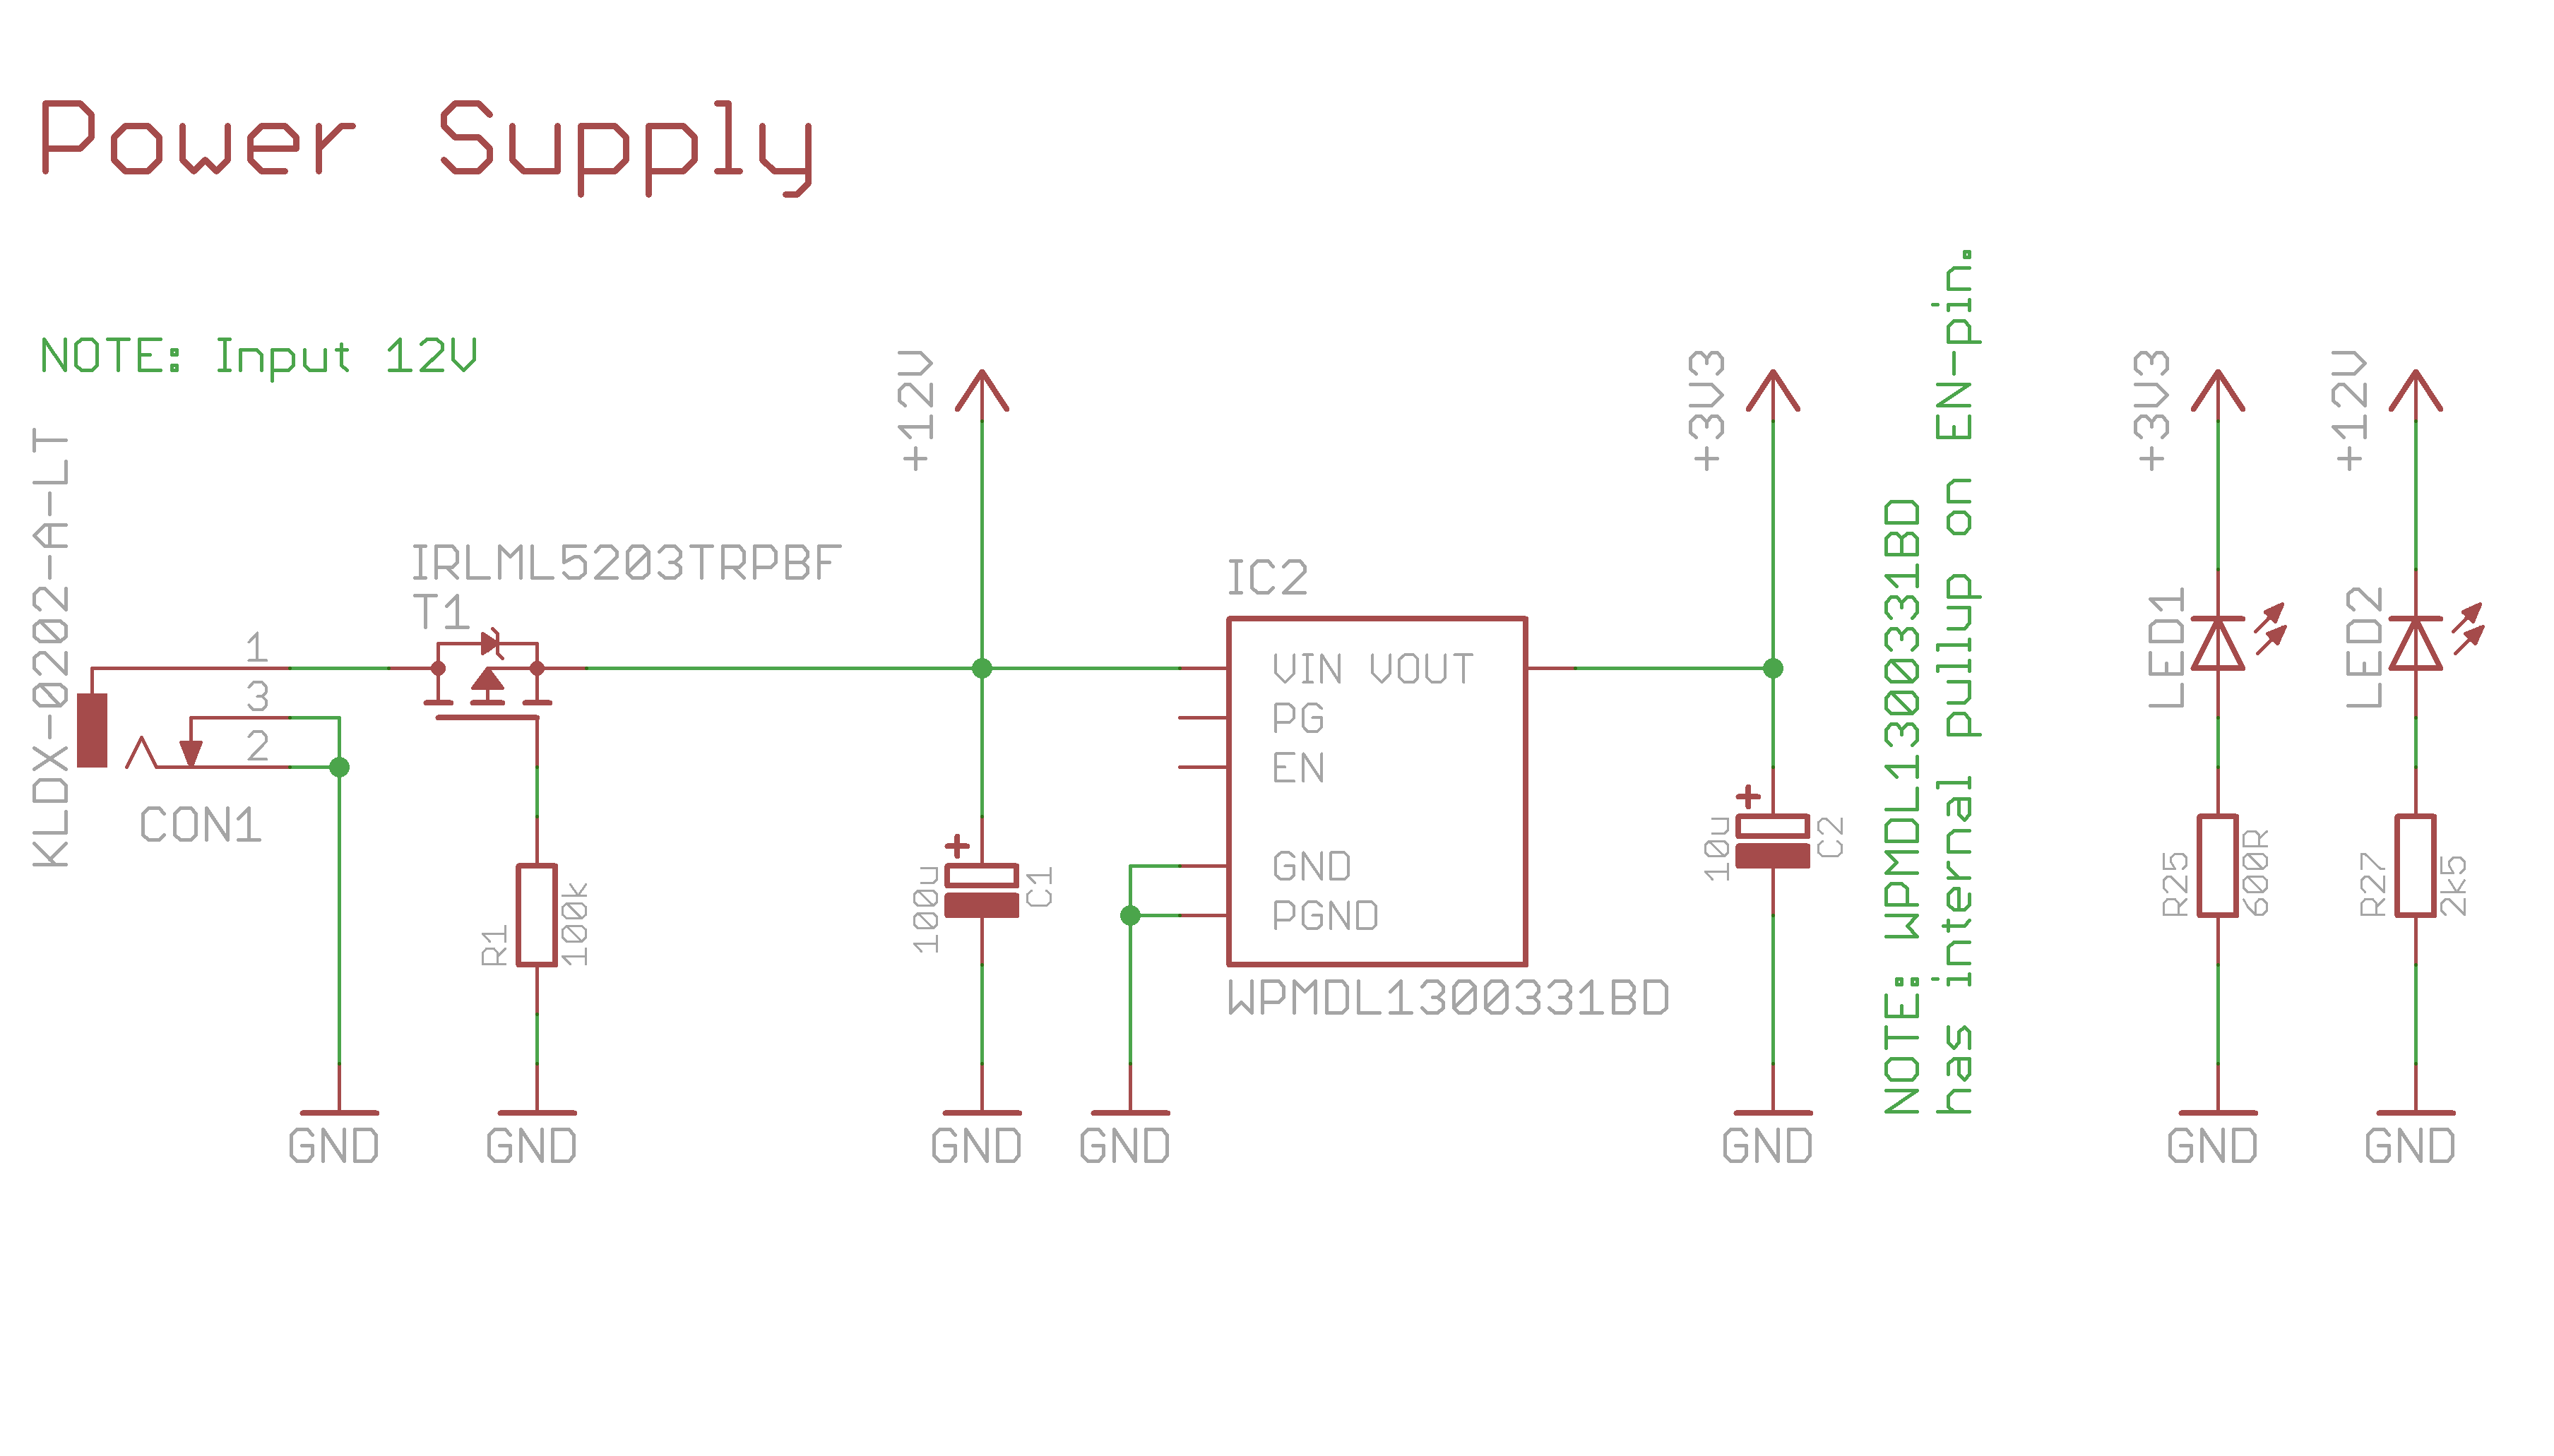
\includegraphics[width=1\textwidth]{TeilB/power_sup_sch.png}}
    \caption{Verpolschutz und Versorgungsspannung +3.3\,V}
    \label{fig:3_3_supply}
\end{figure}\\
Wird eine korrekt gepolte Spannung angelegt, leitet zuerst die Bulk-Diode des P-Kanal MOSFETs. Somit liegt die Eingangsspannung an Source an und die Bedingung ist erfüllt, dass die Source-Spannung um $U_{gsth}$ kleiner wird wird als die Gate-Spannung. Der Transistor leitet nun Strom. Wird aber eine verpolte Spannung angelegt, so sperrt die Bulk-Diode und der Transistor ist nicht in der Lage in einen leitenden Zustand zu gelangen (siehe \cite{Miller2010}). \refa{fig:verpolschutz_sim} zeigt ein Simulationsergebnis des Verpolschutz, bei dem im Wechsel +12\,V und -12\,V am Eingang angelegt werden. Die Grüne Kurve zeigt diese wechselnde Eingangsspannung, die Blaue die Spannung nach dem Verpolschutz. Zu sehen ist, dass sobald die Spannung negativ wird, der Transistor sperrt und die Spannung bei 0\,V liegt.
\begin{figure}[htp]
	\center
	\fbox{	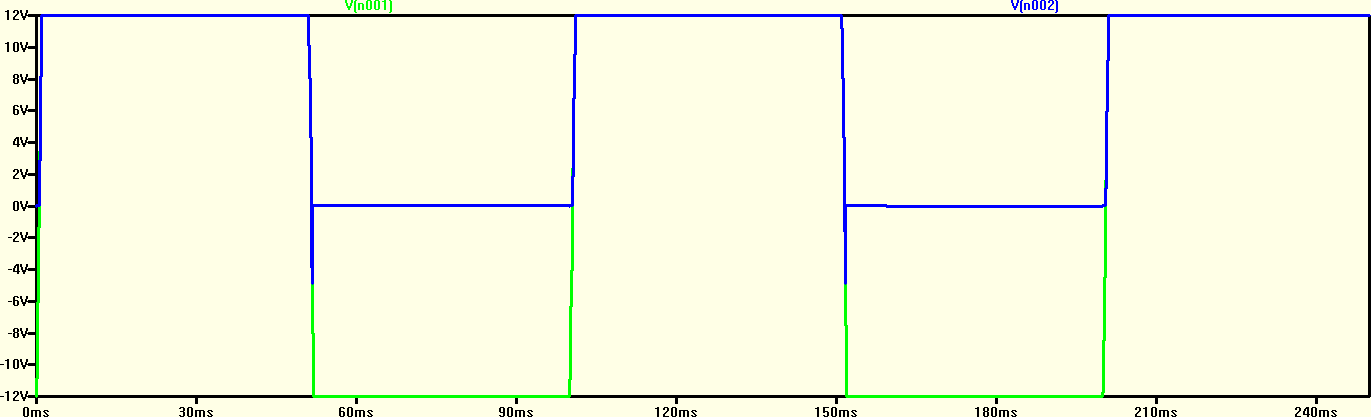
\includegraphics[width=1\textwidth]{TeilB/verpolschutz_messung.png}}
    \caption{Simulation des Verpolschutz}
    \label{fig:verpolschutz_sim}
\end{figure}\\

Die RGB-Bridge \code{TFP401A} sowie die LVDS-Bridge \code{SN65LVDS83B} werden mit +3.3\,V versorgt. Für die Erzeugung der +3.3\,V ist ein voll-integrierter Schaltregler \code{WPMDL1300331BD} von Würth Elektronik im Einsatz. Der Vorteil dieses Schaltreglers ist seine kompakte Bauform und dass keine weiteren externen Bauteile benötigt werden. Der Schaltregler liefert bei +3.3\,V bis zu 3\,A Strom (siehe \cite{Wuerth2013}, S. 4). Wie viel Strom die einzelnen Komponente innerhalb der +3.3\,V-Versorgung benötigen ist \reft{tab:3_3v_strom} zu entnehmen.
\begin{table}[h]
\begin{tabular}{|p{3cm}|p{5cm}|p{4.5cm}|}\hline
\rowcolor{TableBackgroundColor} 
   \textbf{Bauteil} & \textbf{Stromaufnahme} & \textbf{Quelle}	\\ \hline
    TFP401A & 370\,mA & \cite{TI2011}, S. 6\\ \hline
	SN65LVDS83B & 53.3\,mA & \cite{TI2011b}, S. 9\\ \hline
	LB070WV8-SL01 LVDS-Display & 403\,mA + 280\,mA = 683\,mA & \cite{LG2012}, S. 6f\\  \hline
	TY700TFT800480 RGB-Display & 125\,mA + 180\,mA = 305\,mA & \cite{Techtoys2012}, S. 3\\ \hline
\end{tabular}
\caption{Stromaufnahme der +3.3\,V-Versorgung}
\label{tab:3_3v_strom}
\end{table} \\
Wird unter Verwendung des RGB-Displays die LVDS-Bridge nicht auf der Platine bestückt, so errechnet sich die Stromaufnahme aus dem Verbraucht der RGB-Bridge und dem RGB-Display und beläuft sich auf  $370\,mA + 305\,mA = 675\,mA$. Wird die LVDS-Bridge bei gleichen Bedingungen bestückt, so ergibt sich eine maximale Stromaufnahme von $728\,mA$.\\
Im Falle der Verwendung des LVDS-Displays wird die RGB- sowie die LVDS-Bridge benötigt. Die errechnete maximale Stromaufnahme beläuft sich somit auf $370\,mA + 53\,mA + 683\,mA = 1106\,mA$. Die +3.3\,V-Versorgung ist somit für die Anwendung gut dimensioniert.\newline

Der ATMEGA sowie das EEPROM werden durch die HDMI-Buchse versorgt, da diese funktionieren müssen, sobald die Platine angesteuert wird. Laut Spezifikation liefert die HDMI-Buchse bei +5\,V mindestens einen Strom von 55\,mA (siehe \cite{HDMI11}). Der maximale Strom der einzelnen Komponenten ist in \reft{tab:5v_strom} gezeigt und macht in der Summe maximal 15\,mA aus. Die Stromaufnahme ist somit gut im Rahmen der HDMI-Spezifikation.
\begin{table}[h]
\begin{tabular}{|p{4cm}|p{5cm}|p{3.5cm}|}\hline
\rowcolor{TableBackgroundColor} 
   \textbf{Bauteil} & \textbf{Stromaufnahme} & \textbf{Quelle}	\\ \hline
    ATMEGA88 Prozessor & 12\,mA @ 5\,V, 8\,MHz	& \cite{Atmel2011}, S. 3\\ \hline
	AT24C01 EEPROM & 1\,mA lesend, 3\,mA schreibend & \cite{Atmel2003}, S. 303\\ \hline
\end{tabular}
\caption{Stromaufnahme der +5\,V-Versorgung}
\label{tab:5v_strom}
\end{table} \\
Die USB-Bridge \code{FT232RL} wird nur im Falle der erneuten Programmierung des EEPROMs benötigt und deshalb über den USB-Port versorgt. Im Low-Power Modus kann ein USB-Port 100\,mA liefern (siehe \cite{USB2005}, S. 1), was für die Verwendung des FTDI-Chips vollkommen ausreichend ist. Dieser benötigt im Normalbetrieb 15\,mA (siehe \cite{FTDI2010}, S. 18).

In \refc{sec:TeilB_Hardware} ist der Lagenaufbau bereits angesprochen worden. Die Innenlagen sind, mit wenigen Ausnahmen, für die \code{Ground}, \code{+5V} und \code{+3.3V} reserviert. 
\begin{figure}[htbp]
        %\begin{center}
        \centering
        \begin{subfigure}[htp]{0.48\textwidth}
                \fbox{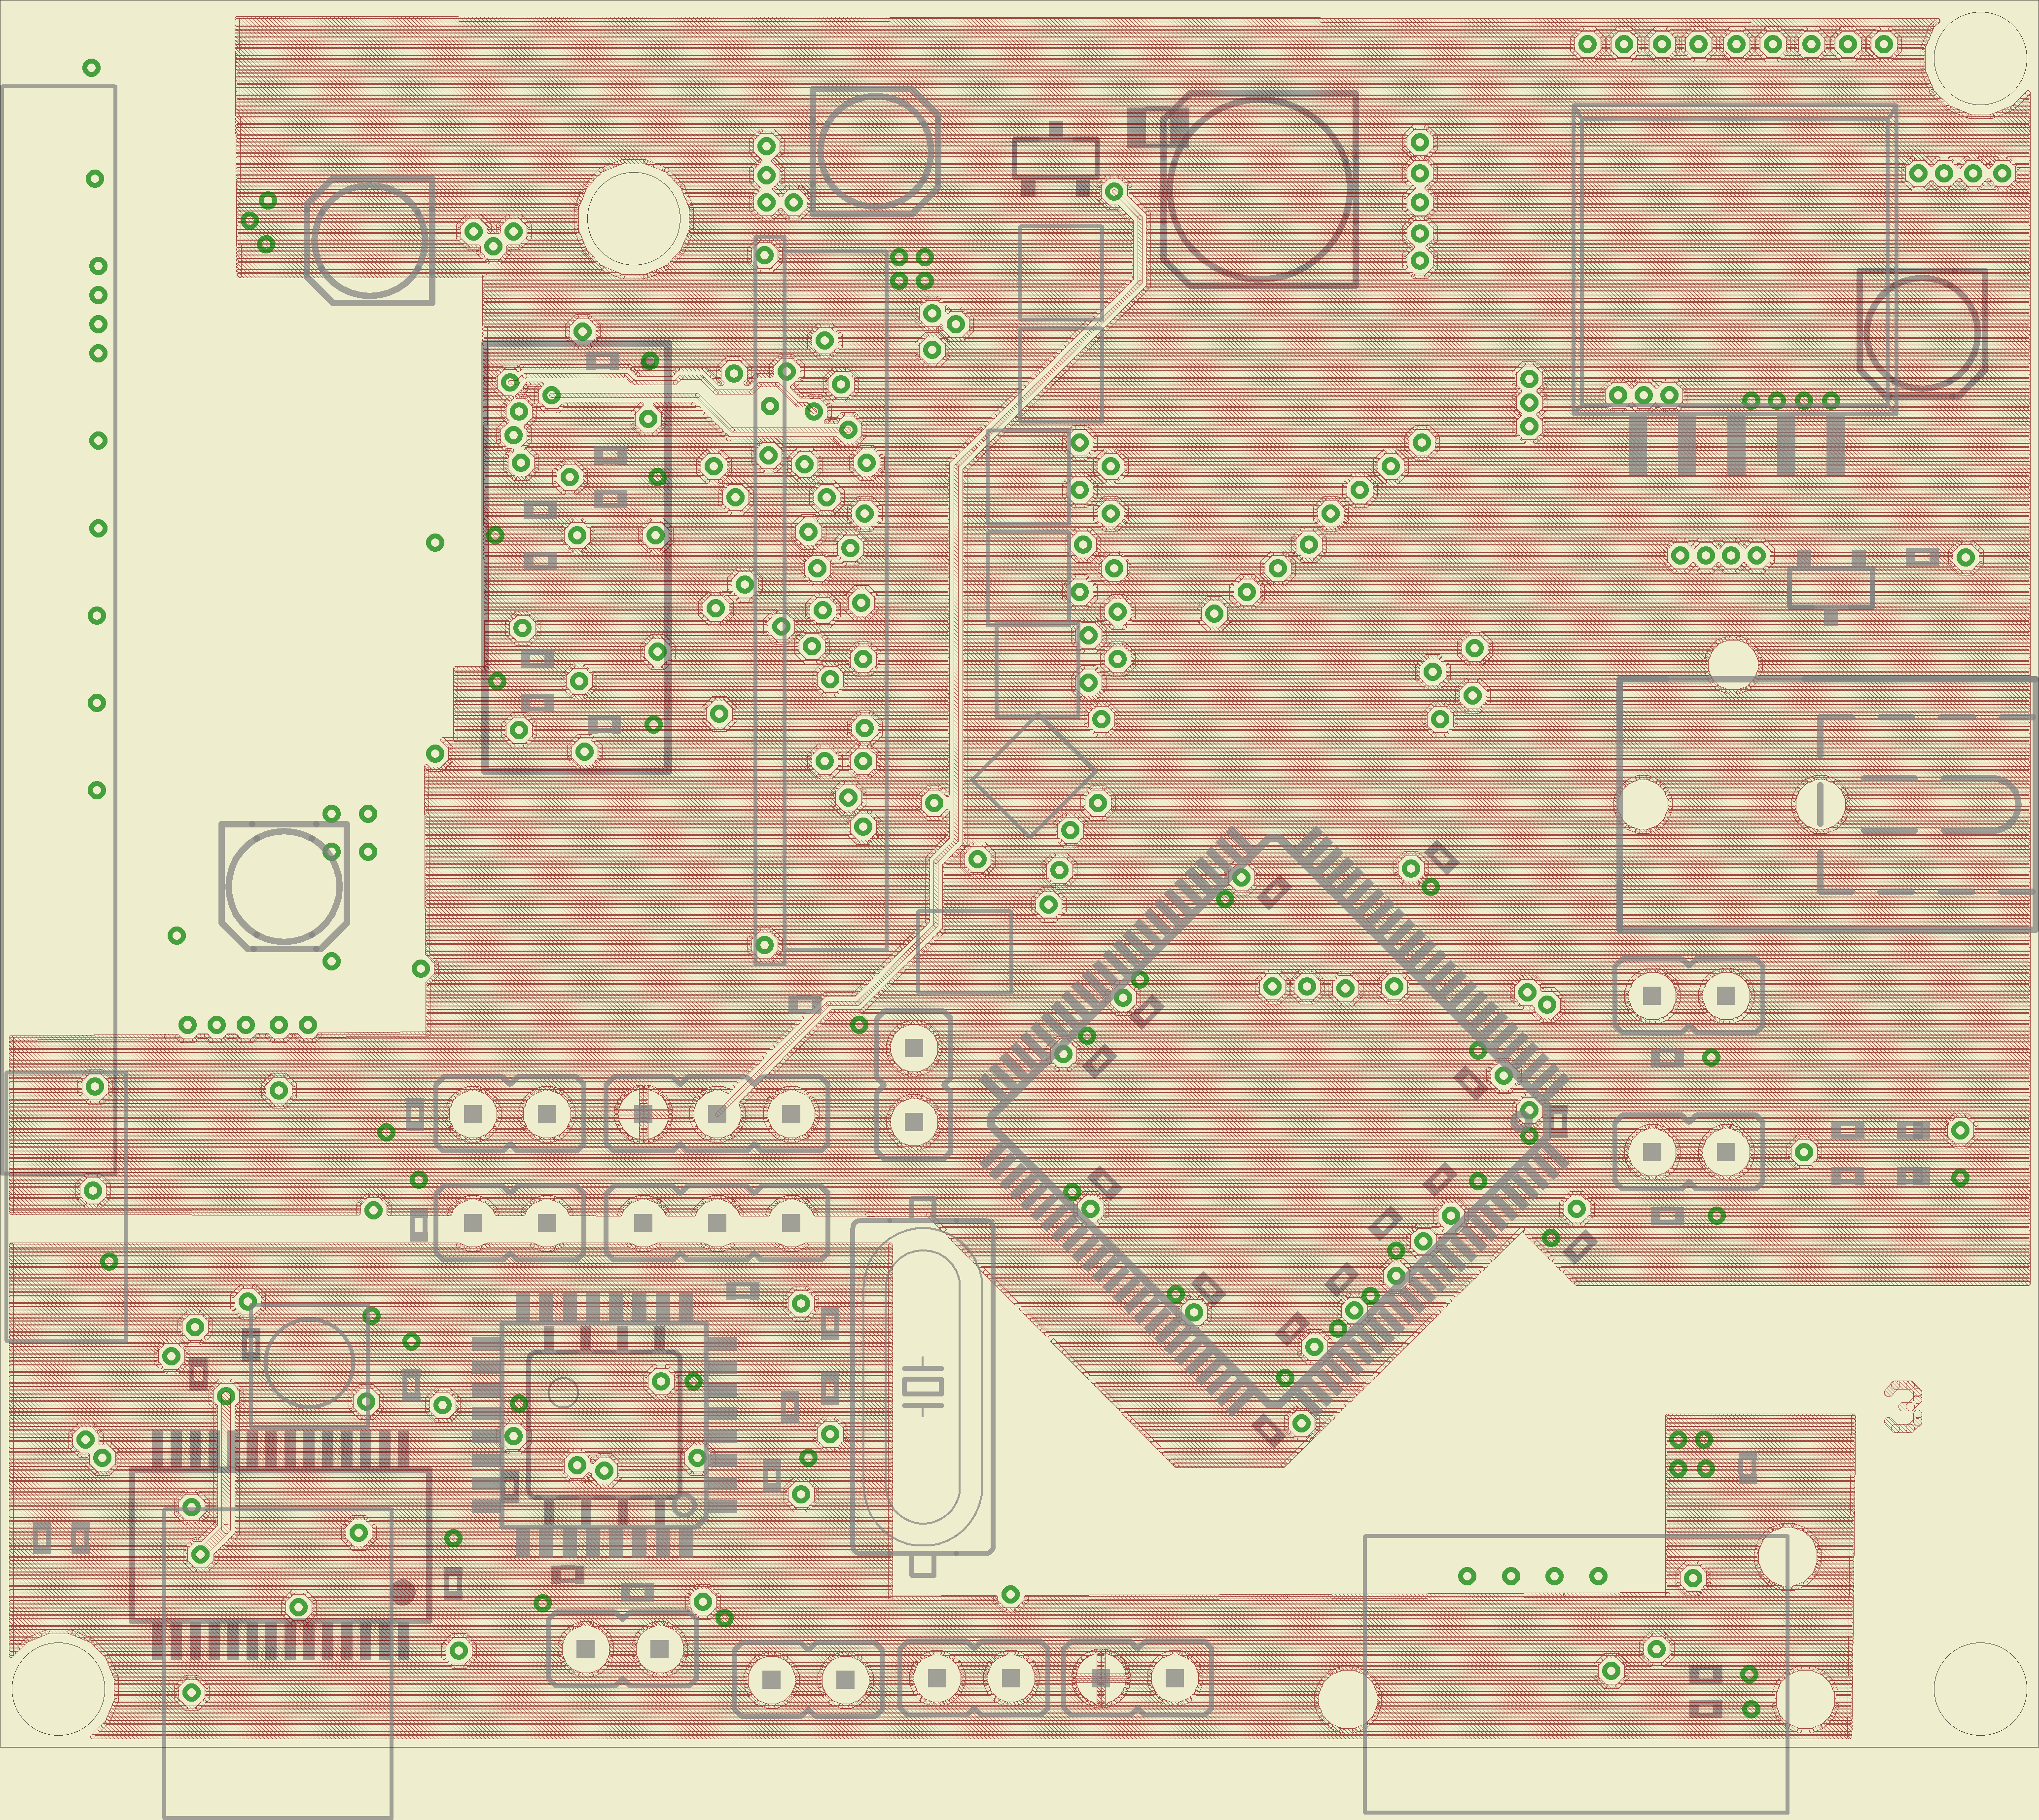
\includegraphics[width=1\textwidth]{TeilB/vcc_layer.png}}
                \caption{Versorgungs-Layer}
                \label{fig:teilb_vcc_layer}
        \end{subfigure}
		\quad 
        \begin{subfigure}[htp]{0.48\textwidth}
               \fbox{ 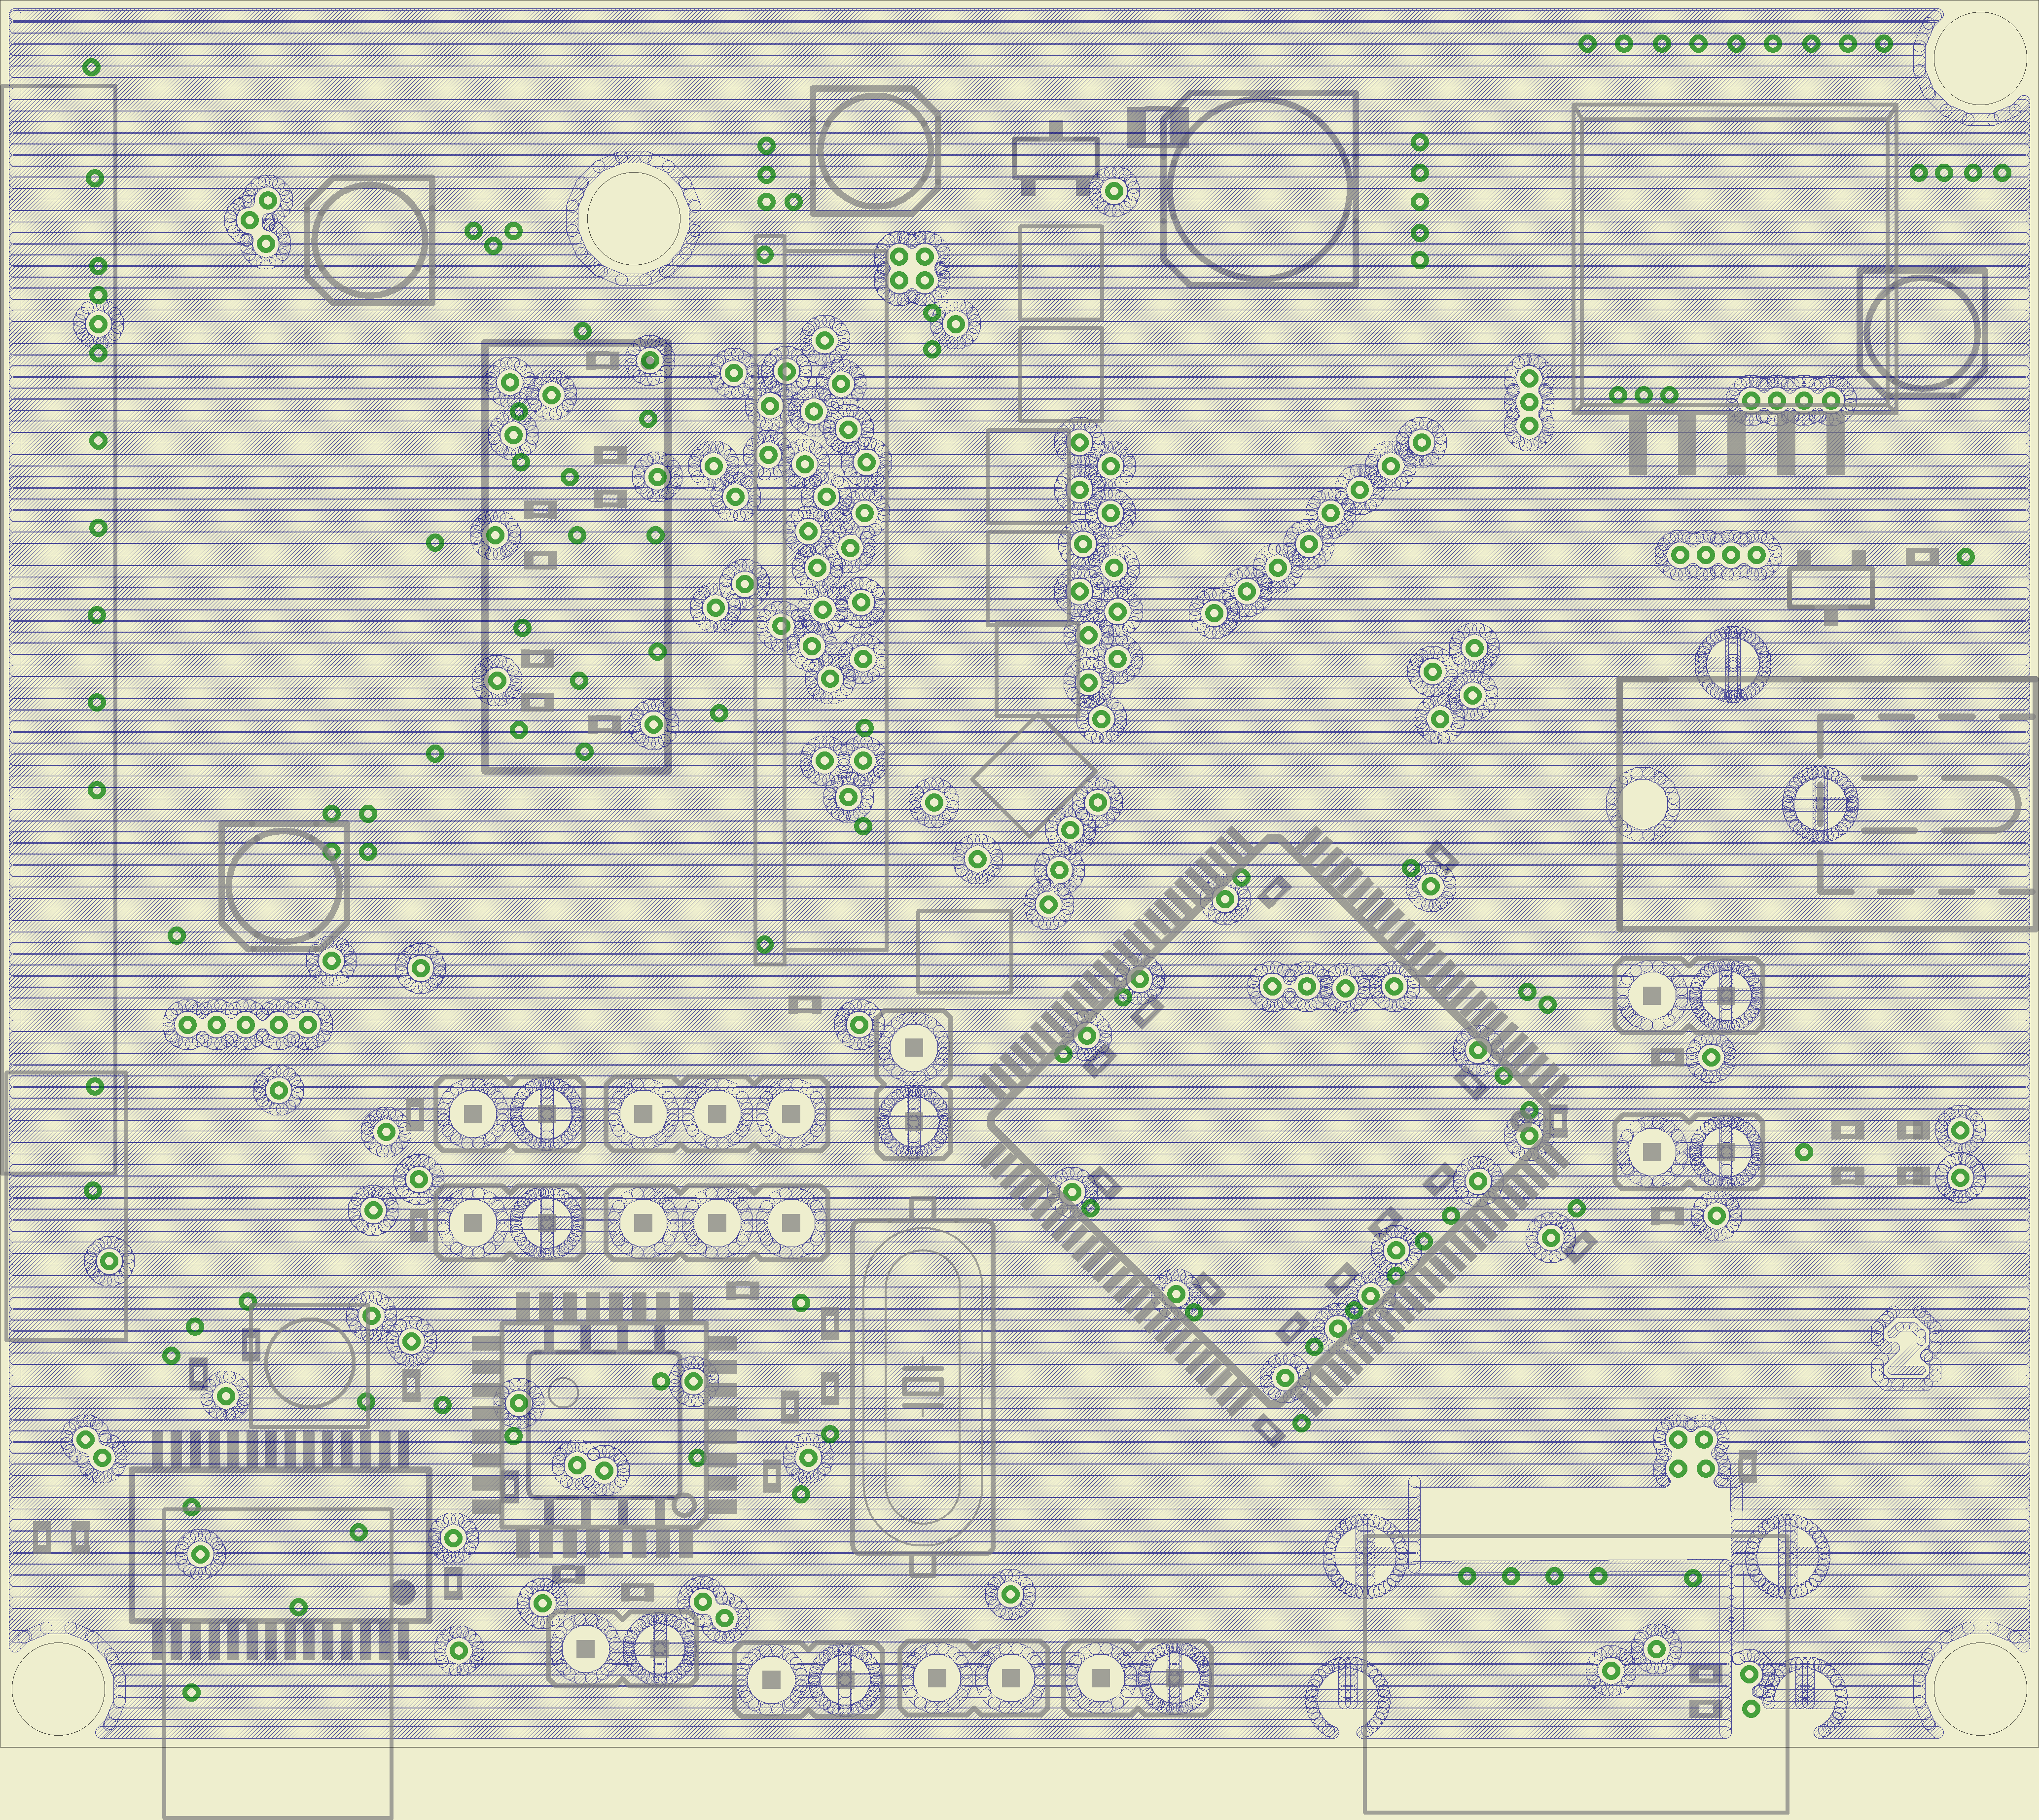
\includegraphics[width=1\textwidth]{TeilB/gnd_layer.png} }              								\caption{Ground-Layer}
                \label{fig:teilb_gnd_layer}
        \end{subfigure}
		%\end{center}
        \caption{Innenlagen}
        \label{fig:teilb_vcc_gnd_layer}
\end{figure}
Die obere Fläche in \refa{fig:teilb_vcc_layer} stellt die +3.3\,V-Versorgung dar. Die Bauteile sind durch kurze Wege mit Vias mit der Lage verbunden. Entsprechend ist die untere Fläche die +5\,V-Versorgung, vom HDMI-Stecker. Die Ground-Fläche ist in \refa{fig:teilb_gnd_layer} zu sehen. Sie umfasst fast die komplette Platine mit Ausnahme unter den Anschlüssen des HDMI-Steckers, da somit die Impedanz der HDMI-Leitungen besser angepasst werden (siehe \cite{TI2007}, S. 7). 
\section{Software}
\label{sec:TeilB_Software}

\subsection{EDID-Daten auf embedded Seite}
\subsubsection{Konzept}
\subsubsection{Low-Level-Treiber}
\paragraph{UART-Treiber}
\paragraph{I2C-Treiber}
\subsubsection{Programmablauf}

\subsection{EDID-Daten auf PC Seite}
\subsubsection{Konzept}
\subsubsection{GTK GUI mit Glade}
\subsubsection{Programmablauf}

\section{Known Bugs}
In den Folgenden Abschnitten wird auf bekannte Fehler eingegangen 
\subsection{Hardware}
\subsubsection{HDMI-Stecker gekreuzt, CON2}
\subsubsection{LVDS-Steckerfootprint gespiegelt, CON6}
\subsubsection{+12V PWM Hintergrundbeleuchtung}
\subsubsection{+5V Kreis / Widerstand R13}
\subsubsection{USB D+/D- vertauscht R22, R23}
\subsection{Software}
\subsubsection{EDID Programmer}

\input{Inhalt/TeilB/TeilBZusammenfassung}
\chapter{Zusammenfassung}
\label{cha:Zusammenfassung}
Die Ziele der beiden Teile dieser Masterarbeit waren
\begin{itemize}
\item Optimierte Portierung des vorausgehenden Projekts zur Ansteuerung von TFT-Displays
\item Ausnutzung der vollen Grafikleistung von Linux-Boards mit Grafikhardware über die HDMI-Schnittstelle über eine selbst entwickelte Hardware zur Ansteuerung von Displays
\end{itemize}
Im Teil A dieser Arbeit ist auf die Low-Level Programmierung des verwendeten Prozessors \code{LPC 3131} eingegangen worden. Es wurde ein Verfahren entwickelt, Displays mit 8080-Interface an einem Speicherbus des Prozessors zu betreiben. Diese Methode findet in einem entwickelten Framebuffer-Treiber im Linux-Kernel, einem User-Space-Treiber sowie im Bootloader Verwendung.\newline

Hierbei ergaben sich Erschwernisse in der Entwicklung, die teilweise gelöst wurden aber noch Fragen bzgl. der Fehlerursachen offen lassen. 
So scheint die Verwendung der Grafikcontroller \code{SSD1963} im Vergleich zum \code{SSD1289} und dem Display \code{MD050SD} in der entwickelten Anwendung nicht nutzbar zu sein. Die Fehlerursache konnte trotz ausgedehnter Suche nach wie vor nicht ermittelt werden.\newline
Mit dem \code{MD050SD} lässt sich das Ziel der optimierten Ansteuerung unter Verwendung des Speicherinterface gut zeigen. Dabei wird gezeigt, dass es auch für leistungsschwache Systeme gute Möglichkeiten zur Anzeige gibt.\newline

Mit der vollen Ausnutzung der Grafikhardware ist das Linux-Board als Einheit zu sehen, welche über die HDMI-Schnittstelle verlassen wird. Die berechneten Video-Signale werden von einer Onboard-Grafikeinheit zur Verfügung gestellt die mit der entwickelten Hardware aus Teil B aufgegriffen und ausgewählte TFT-Displays angeschlossen werden können. Die Schnittstellen zum Anschluss dieser Displays sind der \code{RGB}-Bus sowie ein \code{LVDS}-Interface.\newline
Um einen Plug-And-Play-Betrieb an einer HDMI-Quelle zu ermöglichen, wurden EDID-Daten auf der Platine hinterlegt und die Möglichkeit gegeben, diese mittels USB neu zu beschreiben.\newline
Während der Entwicklung sind ebenfalls Fehler aufgetreten, die teilweise behoben wurden. In der gefertigten Hardware sind diese als Fehler im Schaltplan zu finden.\newline
Dennoch wurde das Ziel der Ausnutzung der vollen Grafikleistung dahingehend erfüllt, dass eine funktionierende Methode entwickelt wurde die HDMI-Signale anzuzeigen wie geplant anzuzeigen.

% \chapter{Zitate und Referenzen}
\label{cha:ZitateReferenzen}

Die \NeuerBegriff{Service-orientierte Architektur} (SOA) ist seit einiger Zeit \textit{das} Schlagwort im Bereich der Informationstechnologie. So haben \zB Deutschlands größte Softwarehersteller SAP und die Software AG ihre Unternehmensstrategie komplett auf die SOA ausgerichtet. \Autor{SAP2007} bietet mit \Fachbegriff{Netweaver} seine marktführende ERP-Software auf Basis von SOA an,\footnote{\Vgl\Zitat[S.~127]{SAP2007}} und die \Autor{Software2007b}, die sich selbst als "`The XML Company"' bezeichnet, erweiterte kürzlich noch einmal ihr bereits durchgängig an der SOA orientiertes Produktportfolio durch den Kauf des amerikanischen Unternehmens webMethods um Lösungen zur Unterstützung von Geschäftsprozessen.\footnote{\Vgl\Zitat{Software2007b}} In einem Atemzug mit der SOA werden häufig Webservices genannt, da sie durch ihre hohe Plattformunabhängigkeit und den Einsatz von Internettechnologie oftmals als Referenzimplementierung für die Services in einer SOA angeführt werden. Doch welche Vorteile bietet der Einsatz von Webservices in Unternehmen? Können mit ihnen tatsächlich flexiblere Softwaresysteme entwickelt werden? Und wie einfach ist die Implementierung von Webservices auf unterschiedlichen Plattformen? Diesen Fragen wird sich der Autor in der vorliegenden Arbeit widmen.

Wie bereits in Kapitel \ref{cha:Einleitung} auf Seite \pageref{cha:Einleitung} erwähnt, ist zur Unterstützung von Geschäftsprozessen der Einsatz von Informationstechnologie notwendig. Der Autor verfolgt mit dieser Arbeit das Ziel, einen Geschäftsprozess \todo{Was ist ein Geschäftsprozess?} mit Hilfe von Webservices zu optimieren. Hierzu wird er in diesem Kapitel eine Einführung in das Thema Webservices und die damit in Zusammenhang stehenden Technologien geben, und auch auf mögliche Einsatzbereiche von Webservices im Rahmen der Geschäftsprozessoptimierung eingehen. Tabelle \ref{tab:ElementeDerEreignisgesteuertenProzesskette} auf Seite \pageref{tab:ElementeDerEreignisgesteuertenProzesskette} zeigt ganz tolle Sachen.

Ich empfehle allen Softwareentwicklern die Lektüre von \Zitat{Goodliffe2007}.

\section{Definitionen}
Die Service-orientierte Architektur ist ein Ansatz der Softwareentwicklung, der sich stark am Konzept der Geschäftsprozesse orientiert und mit Hilfe von Webservices implementiert werden kann. In den beiden folgenden Kapiteln werden beide Begriffe eingehend erläutert, worauf in Kapitel \ref{cha:Fazit} die für die Umsetzung von Webservices benötigten Technologien vorgestellt werden.

\section{Service-orientierte Architektur}
\Autor{OASIS2007}\footnote{Die \NeuerBegriff{Organization for the Advancement of Structured Information Standards} ist nach \Zitat{OASIS2007} ein internationales Konsortium aus über 600 Organisationen, das sich der Entwicklung von E-Business-Standards verschrieben hat. Mitglieder sind \zB IBM, SAP und Sun.} definiert den Begriff \NeuerBegriff{Service-orientierte Architektur} (SOA) wie folgt:
\begin{quote}
"`\textbf{Service Oriented Architecture} [\ldots] is a paradigm for organizing and utilizing distributed \textbf{capabilities} that may be under the control of different ownership domains."'\footnote{\Zitat[S.~8]{OASIS2006a}}
\end{quote}
Diese bewusst allgemein gehaltene Definition stammt aus dem Referenzmodell der SOA aus dem Jahr 2006. Dieses Modell wurde mit dem Ziel entwickelt, ein einheitliches Verständnis des Begriffs SOA und des verwendeten Vokabulars zu schaffen, und sollte die zahlreichen bis dato vorhandenen, teils widersprüchlichen Definitionen ablösen.\footnote{\Vgl\Zitat[S.~4]{OASIS2006a}} Dabei wird zunächst noch kein Bezug zur Informationstechnologie hergestellt, sondern allgemein von Fähigkeiten gesprochen, die Personen, Unternehmen, aber eben auch Computer besitzen und evtl. Anderen anbieten, um Probleme zu lösen. Als Beispiel wird ein Energieversorger angeführt, der Haushalten seine Fähigkeit Strom zu erzeugen anbietet.\footnote{\Vgl\Zitat[S.~8f.]{OASIS2006a}}

% \chapter{Bilder und Listings}

In den folgenden drei Kapiteln wird der Autor eine einfache Webservice-Umgebung aufbauen, um zu zeigen, wie Webservices in der Praxis angeboten, konsumiert und orchestriert werden k�nnen. Hierzu verwendet er ausschlie�lich Open-Source-Software, im Speziellen \NeuerBegriff{Apache Tomcat}\footnote{Website: \url{http://tomcat.apache.org/}} als Servlet-Engine, \NeuerBegriff{Apache Axis2}\footnote{Website: \url{http://ws.apache.org/axis2/}} als SOAP-Engine und \NeuerBegriff{ActiveBPEL}\footnote{Website: \url{http://www.activebpel.org/}} als Workflow-System. Die Installation und Konfiguration der ben�tigten Anwendungen wird in Kapitel \ref{sec:Werkzeuge} beschrieben. Die komplette Umgebung inkl. der vom Autor erstellten Webservices befindet sich als virtuelle Maschine auf der dieser Arbeit beigelegten DVD. Im Folgenden wird der DNS-Name \Code{linux-ws} als Bezeichnung f�r den Webservice-Server verwendet.

\section{Anbieten eines Webservice}
\label{sec:AnbietenEinesWebservices}
Mit Hilfe von Apache Axis2 k�nnen Webservices sehr einfach auf Basis von normalen Java-Klassen angeboten werden. Es ist lediglich eine zus�tzliche XML-Datei namens \Datei{META-INF/services.xml} n�tig, in der die zu ver�ffentlichenden Klassen und Methoden beschrieben werden. \abbildung{HelloWorldStruktur} zeigt die Struktur eines einfachen \Webservice{HelloWorld}-Webservice.

\begin{figure}[htb]
\centering
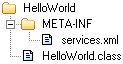
\includegraphics[width=0.3\textwidth]{HelloWorldStruktur.jpg}
\caption{\Webservice{HelloWorld}-Webservice: Dateistruktur}
\label{fig:HelloWorldStruktur}
\end{figure}

Die Klasse \Code{HelloWorld} besitzt nur die Methode \Code{SayHello}, die den \Datentyp{String} \Code{Hello World!} zur�ckgibt. Sie wird in Listing \ref{lst:HelloWorldJava} gezeigt. 

\newpage
\lstset{language=Java, basicstyle=\footnotesize, showstringspaces=false, tabsize=2}
\lstinputlisting[label=lst:HelloWorldJava,caption=\Webservice{HelloWorld}-Webservice: Java-Klasse \Code{HelloWorld}]{DVD/Listings/HelloWorld/HelloWorld.java}

\section{Netzwerkverkehr beim Aufruf von \Webservice{PersonFactory}}

\subsection{SOAP-Request}
Listing \ref{lst:SOAPRequest} zeigt die mitgeschnittene SOAP-Anfrage per HTTP an den Webservice \Webservice{PersonFactory}. Wie am Ende von Kapitel \ref{cha:Einleitung} beschrieben, wird die eigentliche SOAP-Nachricht mittels des HTTP-\Eingabe{POST}-Befehls (Zeile 1) an den Webservice unter der angegebenen URL (Zeile 1) auf dem Server (Zeile 5) geschickt. In Zeile 3 wird �ber den Befehl \Eingabe{SOAPAction} �bermittelt, welche Funktion des Webservice (in diesem Fall \Code{CreatePerson}) aufgerufen werden soll. Die XML-Nutzlast (Zeilen 8--18) besteht dann aus einer einfachen SOAP-Nachricht aus \XMLElement{Envelope}, \XMLElement{Header} und \XMLElement{Body}, die einen RPC durchf�hrt. Die aufzurufenden Funktion wird noch einmal im SOAP-\XMLElement{Body} in Zeile 15 definiert.


\lstset{language=XML, basicstyle=\footnotesize, showstringspaces=false, tabsize=2}
\lstinputlisting[label=lst:SOAPRequest,caption=SOAP-Request an \Webservice{PersonFactory} per HTTP]{DVD/Listings/PersonFactorySOAPRequest.txt}

\subsection{SOAP-Response}
Die Antwort des \Webservice{PersonFactory}-Webservice zeigt Listing \ref{lst:SOAPResponse}. Sie beginnt in Zeile 1 mit dem HTTP-Statuscode 200, der die Anfrage als erfolgreich kennzeichnet. Die eigentliche Nutzlast in Form von XML-Daten (Zeile 3) folgt dann ab Zeile 7. Sie besteht aus dem Element \XMLElement{Person} und seinen Unterelementen, umschlossen vom Element \XMLElement{CreatePersonRepsonse}, das die Antwort-Nachricht aus der WSDL repr�sentiert.

\lstset{language=XML, basicstyle=\footnotesize, showstringspaces=false, tabsize=2}
\lstinputlisting[label=lst:SOAPResponse,caption=SOAP-Response von \Webservice{PersonFactory} per HTTP]{DVD/Listings/PersonFactorySOAPResponse.txt}

% \chapter{Aufz�hlungen und Tabellen}

Eine normale Punktliste:
\begin{itemize}
\item Lorem ipsum dolor sit amet, consectetuer adipiscing elit. Nulla ac ipsum a metus viverra tempor. 
\item Nunc sem. Nulla nec urna eu nibh vehicula convallis. Integer ac turpis. Donec mauris enim, dignissim quis, scelerisque ac, rhoncus id, sapien. 
\item Donec turpis felis, cursus in, varius vitae, mollis ac, lorem. Integer a dui sit amet eros nonummy aliquet. Donec egestas adipiscing tellus. Nulla iaculis. 
\item Aliquam erat volutpat. Curabitur posuere, eros vitae accumsan semper, risus erat viverra erat, eu vehicula mi leo at elit. Fusce luctus. Fusce vehicula pretium diam. Nunc sed arcu ut erat suscipit fermentum.
\end{itemize}

Eine nummerierte Liste:
\begin{enumerate}
\item Lorem ipsum dolor sit amet, consectetuer adipiscing elit. Nulla ac ipsum a metus viverra tempor. 
\item Nunc sem. Nulla nec urna eu nibh vehicula convallis. Integer ac turpis. Donec mauris enim, dignissim quis, scelerisque ac, rhoncus id, sapien. 
\item Donec turpis felis, cursus in, varius vitae, mollis ac, lorem. Integer a dui sit amet eros nonummy aliquet. Donec egestas adipiscing tellus. Nulla iaculis. 
\item Aliquam erat volutpat. Curabitur posuere, eros vitae accumsan semper, risus erat viverra erat, eu vehicula mi leo at elit. Fusce luctus. Fusce vehicula pretium diam. Nunc sed arcu ut erat suscipit fermentum.
\end{enumerate}

\section{Vom Autor verwendete Software}
\label{sec:Werkzeuge}
Im Folgenden werden die Programme vorgestellt, die der Autor zum Erstellen dieser Arbeit und vor allem zur Entwicklung der Webservices verwendet hat. Soweit es m�glich war, wurden Open-Source-Programme eingesetzt.

\begin{itemize}
\itemd{Microsoft Visio}{Die EPKs der BAP wurden mit Microsoft Visio erstellt. Der Autor hat zwar verschiedene Open-Source-Programme\footnote{Dia, OpenOffice Draw und die EPC Tools.} ausprobiert, mit denen EPKs erstellt werden k�nnten, die grafischen Ergebnisse waren aber nicht zufriedenstellend. Die Symbole von Visio sehen den "`originalen"' ARIS-Symbolen am �hnlichsten und k�nnen dar�ber hinaus mit zus�tzlichen Informationen wie Dauer und Kosten versehen werden.}
\itemd{PSPad}{F�r die Bearbeitung von verschiedenen (Text-)Dateien wurde der Texteditor PSPad verwendet. Mit diesem konnten \zB auch die regul�ren Ausdr�cke f�r die XML-Schemas entwickelt werden. Website: \url{http://www.pspad.com/}}
\itemd{Eclipse}{Sowohl der ActiveBPEL Designer als auch die EntireX Workbench sind Plugins f�r die IDE Eclipse. Auch zur Java- und PHP-Entwicklung wurde dieses Werkzeug verwendet. Website: \url{http://www.eclipse.org/}}
\itemd{XML Copy Editor}{F�r die Entwicklung der XML-Schemas und die Bearbeitung von XML-Dateien wurde der XML Copy Editor eingesetzt. Mit diesem k�nnen \ua XML-Dateien auf Wohlgeformtheit gepr�ft und gegen ihr Schema validiert werden. Website: \url{http://xml-copy-editor.sourceforge.net/}}
\itemd{soapUI}{
Mit soapUI k�nnen Webservices getestet werden, ohne einen Client zu programmieren. Die SOAP-Anfragen werden automatisch anhand der WSDL generiert und die Antworten k�nnen gegen die WSDL-Datei validiert werden. Website: \url{http://www.soapui.org/}}
\itemd{Ethereal}{
Die Netzwerkkommunikation beim Aufrufen der Webservices wurde mit Ethereal, einem umfangreichen Werkzeug zur Analyse des Netzwerkverkehrs, mitgeschnitten. Website: \url{http://www.ethereal.com/}}
\itemd{\LaTeX}{
Diese Arbeit wurde mit {\LaTeX} geschrieben. Als Distribution wurde MiKTeX verwendet und als Editor der LaTeX Editor. Websites: \url{http://miktex.org/}, \url{http://www.latexeditor.org/}}
\end{itemize}

\section{Elemente der Ereignisgesteuerten Prozesskette}

\begin{longtable}{|m{10cm}|m{3cm}|}
\caption{Elemente der Ereignisgesteuerten Prozesskette} \\
\hline
\label{tab:ElementeDerEreignisgesteuertenProzesskette}
\textbf{Element} & \textbf{Symbol}\\
\hline
\textbf{Funktion} 

Funktionen beschreiben T�tigkeiten, die im Verlauf des Gesch�ftsprozesses anfallen. Sie k�nnen von Mitarbeitern oder einem Informationssystem durchgef�hrt werden und ben�tigen evtl. Ressourcen, die ihnen zugewiesen werden. 

Beispiele: \textit{Auftrag anlegen}, \textit{Rechnung schreiben}, \textit{Konto abschlie�en} & 
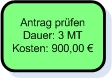
\includegraphics[width=3cm]{EPK-Funktion.jpg} \\
\hline
\textbf{Ereignis} 

Ereignisse sind betriebswirtschaftlich relevante Ereignisse, die den Gesch�ftsprozess in irgendeiner Weise steuern oder beeinflussen. Ereignisse sind immer Ausl�ser oder Ergebnisse von Funktionen. Ein Gesch�ftsprozess beginnt und endet stets mit einem Ereignis. 

Beispiele: \textit{Auftrag eingetroffen}, \textit{�berweisung get�tigt}, \textit{Rechnung erstellt} & 
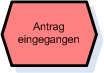
\includegraphics[width=3cm]{EPK-Ereignis.jpg} \\
\hline
\textbf{Operatoren} 

Operatoren steuern den Kontrollfluss eines Gesch�ftsprozesses. Sie machen \zB deutlich, dass eine Funktion mehrere Ereignisse ausl�st, oder zeigen alternative Vorgehensweisen an. Es gibt drei Operatoren (v.\,l.\,n.\,r.\,): UND, ODER und XODER (exklusives ODER). & 

\includegraphics[width=3cm]{EPK-Operatoren.jpg} \\
\hline
\textbf{Organisationseinheit} 

Organisationseinheiten werden Funktionen zugeordnet und beschreiben, wo die Funktionen ausgef�hrt werden bzw. wer sie ausf�hrt. Die Bezeichnung der Symbole enth�lt zus�tzlich zur Abteilung noch die Namen der Mitarbeiter.

Beispiele: \textit{Vertrieb}, \textit{Personal}, \textit{Produktion} & 
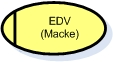
\includegraphics[width=3cm]{EPK-Organisationseinheit.jpg} \\
\hline
\textbf{Informationsobjekt} 

Auch Informationsobjekte werden Funktionen zugewiesen und beschreiben die von diesen ben�tigten oder erstellten Informationen. Dabei sind s�mtliche Formen von Informationen auf verschiedenen Datentr�gern m�glich und nicht etwa nur digitale Daten. Die Bezeichnung der Symbole enth�lt zus�tzlich das Informationssystem, aus dem die Informationen stammen.

Beispiele: \textit{Kundendatenbank}, \textit{Versicherungsantrag}, \textit{Rechnung} & 
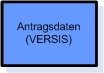
\includegraphics[width=3cm]{EPK-Informationen.jpg} \\
\hline
\textbf{Prozesswegweiser}

Mit Prozesswegweisern werden Prozesse, die in anderen EPKs beschrieben sind, referenziert. So k�nnen \zB un�bersichtliche Prozesse in Teilprozesse gegliedert und h�ufig verwendete Prozesse an zentraler Stelle modelliert werden. Prozesswegweiser stehen in einer EPK immer anstelle von Funktionen. & 
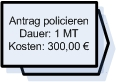
\includegraphics[width=3cm]{EPK-Prozesspfad.jpg} \\
\hline
\end{longtable}

% \chapter{Fazit und kritische Bewertung}
\label{cha:Fazit}
Lorem ipsum dolor sit amet, consectetuer adipiscing elit. Nulla ac ipsum a metus viverra tempor. Nunc sem. Nulla nec urna eu nibh vehicula convallis. Integer ac turpis. Donec mauris enim, dignissim quis, scelerisque ac, rhoncus id, sapien. Donec turpis felis, cursus in, varius vitae, mollis ac, lorem. Integer a dui sit amet eros nonummy aliquet. Donec egestas adipiscing tellus. Nulla iaculis. Aliquam erat volutpat. Curabitur posuere, eros vitae accumsan semper, risus erat viverra erat, eu vehicula mi leo at elit. Fusce luctus. Fusce vehicula pretium diam. Nunc sed arcu ut erat suscipit fermentum.

Proin id magna eu sem tincidunt feugiat. Sed tincidunt massa sed eros. Fusce condimentum eros et lectus. Pellentesque lectus tortor, mattis in, dapibus a, lobortis ut, justo. Sed id dolor ut nibh varius ultrices. Quisque tincidunt nisl vel nibh. Suspendisse sodales massa non magna. In porttitor augue nonummy nunc. Nam quis enim quis ante dapibus interdum. Morbi nec neque. Fusce pharetra consectetuer magna. Etiam laoreet, augue nec lacinia ornare, risus purus lobortis erat, eu consequat urna orci vel arcu. Integer cursus, augue sed tempor dapibus, erat tortor rutrum elit, sit amet fermentum purus neque vitae tortor. Donec vulputate, ipsum vel viverra pretium, purus orci mattis nulla, nec tincidunt leo metus sed ipsum. Fusce eget lectus sed lectus molestie tincidunt. Etiam tincidunt urna eget tortor.

Sed sit amet magna at lectus interdum blandit. Proin vitae metus eget leo bibendum ornare. Morbi sit amet nisl ac odio accumsan laoreet. Etiam luctus massa vel enim. Vestibulum nulla tellus, viverra at, malesuada vel, volutpat quis, lorem. Vestibulum quis nulla. Curabitur neque nibh, bibendum vel, eleifend sit amet, euismod at, leo. Duis auctor lobortis justo. Donec in tortor vel nibh rutrum pellentesque. Curabitur blandit pede quis neque. Nam sem eros, ornare a, pretium eget, condimentum sed, leo. Curabitur orci felis, elementum eget, aliquet vel, porta id, velit. Etiam justo neque, rhoncus quis, elementum vel, auctor vitae, urna.


